% =====================================================================
%  Monografia de Trabalho de Conclusão de Curso I
%  Tema: Verificação formal de invariantes de sessão em data grids:
%        replicação assíncrona, failover e controle orientado a SLO
%  Autor: Francesco Pagani Galvão
%  Orientador: Prof. Dr. Leonardo Bidese de Pinho
%  Universidade Federal do Pampa, Bacharelado em Engenharia de Computação
%  Campus Bagé
% =====================================================================
\documentclass[tcc,baec]{unipampa}

\usepackage[T1]{fontenc}
\usepackage[utf8]{inputenc}
\usepackage{graphicx}
\usepackage{times}
\usepackage{mathptmx}
\usepackage{amssymb}
\usepackage{amsmath}
\usepackage{enumitem}
\usepackage{booktabs}
\usepackage{caption}
\usepackage{longtable}

\usepackage[alf,abnt-emphasize=bf]{abntex2cite}

% Compatibilidade natbib: o abntex2cite (opção alf) já define \citet e \citep,
% mas não \citealt/\citealp. Mapeiam-se para \citeonline (forma "Autor (ano)"),
% coerente com \citet, evitando "Undefined control sequence" nas chamadas.
\providecommand{\citealt}{\citeonline}
\providecommand{\citealp}{\citeonline}

% ---------------------------------------------------------------------
% Identificação do trabalho
% ---------------------------------------------------------------------
\title{Verificação formal de invariantes de sessão em data grids: replicação assíncrona, failover e controle orientado a SLO}
\author{Galvão}{Francesco Pagani}
\advisor[Prof.~Dr.]{Pinho}{Leonardo Bidese de}

% Sem coorientador.
% Banca examinadora (o orientador entra automaticamente via \advisor; abaixo só os demais membros).
% \banca e \inst são posicionais: cada \banca é pareado com o \inst seguinte na folha de aprovação.
\banca[Prof.\ Dr.\ Bruno Silveira Neves]{}{}
\inst{UNIPAMPA}
\banca[Prof.\ Dr.\ Diego Leonel Cadette Dutra]{}{}
\inst{UFRJ}

\cutter{---}
\location{Bagé}{RS}

% Data de publicação (mês e ano que aparecem na folha de rosto / capa).
\date{Outubro}{2026}

% Data de defesa ainda não fixada: campos em branco na folha de aprovação.
% A classe exige \defesa definido para compor a folha; não remover a linha.
\defesa{\underline{\hspace{1cm}}}{\underline{\hspace{3cm}}}{\underline{\hspace{1.2cm}}}

% ---------------------------------------------------------------------
% Palavras-chave (idioma do documento, português)
% ---------------------------------------------------------------------
\keyword{data grid}
\keyword{replicação assíncrona}
\keyword{failover}
\keyword{model checking}
\keyword{invariantes de sessão}
\keyword{objetivos de nível de serviço}

\sloppy

% Marcadores invisíveis de revisão (fusão banca TCC I x versão de 30/10).
% Só registram a página no .aux; são removidos na versão limpa.
\newcommand{\revini}[1]{\label{revini-#1}}
\newcommand{\revfim}[1]{\label{revfim-#1}}

\begin{document}

\maketitle

%
% Dedicatoria (opcional)
%

% \begin{dedicatoria}
% Dedico este trabalho ao meu gato, ao meu cachorro e ao meu papagaio.
% \end{dedicatoria}

%
% Agradecimentos (opcional)
%
% Se você tiver muito a agradecer, pode usar um arquivo à parte e incluí-lo
% no texto, por meio do comando \input{meus-agradecimenos}. O compilador
% LaTeX buscará o arquivo meus-agradecimentos.tex e incluirá o texto do mesmo
% neste local. Isso ajuda a tornar o arquivo principal do trabalho (este)
% mais limpo, claro e conciso.
%

% \chapter*{Agradecimento}
% Agradeço à Antarctica pelas Brahminhas que eles mandaram.

%
% Epígrafe (opcional)
%
% \begin{epigrafe}
% ``If I have seen farther than others, it is because I stood on the shoulders of giants.''\\
% --- Sir~Isaac Newton
% \end{epigrafe}

\begin{abstract}
Aplicações distribuídas costumam delegar o estado de sessão de seus usuários a um \emph{data grid} replicado, que funciona como camada de sessão compartilhada entre vários nós. Como a replicação é assíncrona para sustentar o desempenho dessa camada, uma atualização aplicada em um nó leva algum tempo até alcançar todas as réplicas, e nesse intervalo as réplicas permanecem temporariamente divergentes. Se um nó cai antes que a última atualização chegue às demais réplicas, o \emph{failover} pode promover uma réplica desatualizada e reverter efeitos que já deveriam ser definitivos, fazendo um \emph{logout} voltar a valer, um contador de tentativas regredir ou um bloqueio desaparecer. Essas falhas comprometem segurança e cumprimento de SLO e escapam ao teste convencional porque dependem de entrelaçamentos específicos entre operações concorrentes e eventos de falha. Este trabalho formaliza tais propriedades como invariantes de sessão, entre elas a irreversibilidade do \emph{logout}, a persistência do bloqueio, a não regressão do contador de tentativas e a convergência do estado, e investiga sob que condições essas garantias resistem ou se rompem diante de replicação assíncrona e \emph{failover}. A proposta especifica formalmente o protocolo e o estado de sessão, aplica verificação de modelos para identificar as condições sob as quais cada invariante falha e, a partir dessas condições, projeta um algoritmo de decisão que atua em tempo de execução sobre as políticas e os parâmetros de configuração do \emph{cluster}, ajustando-os conforme as falhas observadas para reduzir violações e controlar a cauda de latência. Esse controle adaptativo da configuração em \emph{runtime} é o eixo da proposta, pela qual o trabalho intervém sobre o compromisso entre correção do estado e latência. A avaliação apoia-se em verificação de modelos e em experimentação sobre um \emph{cluster} real submetido a falhas induzidas, confrontando o comportamento observado com o que a especificação indica. O trabalho pretende oferecer garantias de correção do estado de sessão sob falhas em \emph{data grids} replicados sem sacrificar os SLO de latência acordados.
\end{abstract}

\begin{englishabstract}{Data grid, asynchronous replication, failover, model checking, session invariants, service level objectives}
Distributed applications often delegate their users' session state to a replicated \emph{data grid} that acts as a shared session layer across several nodes. Because replication runs asynchronously to sustain the performance of that layer, an update applied on one node takes some time to reach every replica, and during this interval the replicas remain temporarily divergent. If a node fails before the latest update reaches the other replicas, \emph{failover} may promote a stale replica and revert effects that should already be final, making a \emph{logout} valid again, a login attempt counter regress or a lockout disappear. Such faults compromise security and SLO compliance and escape conventional testing because they depend on specific interleavings between concurrent operations and failure events. This work formalizes these properties as session invariants, among them the irreversibility of \emph{logout}, the persistence of lockout, the non-regression of the attempt counter and state convergence, and investigates under which conditions these guarantees hold or break under asynchronous replication and \emph{failover}. The proposal formally specifies the session protocol and state, applies model checking to identify the conditions under which each invariant fails and, from these conditions, designs a decision algorithm that acts at run time over the policies and configuration parameters of the \emph{cluster}, tuning them according to the observed faults to reduce violations and control the latency tail. This adaptive control of the cluster configuration at runtime is the core of the proposal, through which the work intervenes on the trade-off between state correctness and latency. The evaluation relies on model checking and on experimentation over a real \emph{cluster} subjected to induced faults, confronting the observed behavior with what the specification indicates. The work aims to offer guarantees of session state correctness under faults in replicated \emph{data grids} without sacrificing the agreed latency SLO.
\end{englishabstract}

\listoffigures
\listoftables

% Lista de abreviaturas e siglas
\begin{listofabbrv}{ABNT}
    \item[ABNT]     \ \ \ \ \ \ \ \ \ \ \ \ \ Associação Brasileira de Normas Técnicas
    \item[ACM]      \ \ \ \ \ \ \ \ \ \ \ \ \ \emph{Association for Computing Machinery}
    \item[CAP]      \ \ \ \ \ \ \ \ \ \ \ \ \ \emph{Consistency, Availability, Partition tolerance}
    \item[CPU]      \ \ \ \ \ \ \ \ \ \ \ \ \ \emph{Central Processing Unit}
    \item[CRDT]     \ \ \ \ \ \ \ \ \ \ \ \ \ \emph{Conflict-free Replicated Data Type}
    \item[FLP]      \ \ \ \ \ \ \ \ \ \ \ \ \ Fischer, Lynch e Paterson
    \item[IEEE]     \ \ \ \ \ \ \ \ \ \ \ \ \ \emph{Institute of Electrical and Electronics Engineers}
    \item[IMDG]     \ \ \ \ \ \ \ \ \ \ \ \ \ \emph{In-Memory Data Grid}
    \item[JVM]      \ \ \ \ \ \ \ \ \ \ \ \ \ \emph{Java Virtual Machine}
    \item[LWW]      \ \ \ \ \ \ \ \ \ \ \ \ \ \emph{Last Writer Wins}
    \item[MAPE-K]   \ \\ \ \ \ \ \ \ \ \ \ \ \emph{Monitor, Analyze, Plan, Execute over Knowledge}
    \item[NIST]     \ \ \ \ \ \ \ \ \ \ \ \ \ \emph{National Institute of Standards and Technology}
    \item[OWASP]    \ \ \ \ \ \ \ \ \ \ \ \ \ \emph{Open Worldwide Application Security Project}
    \item[PRISMA]   \ \ \ \ \ \ \ \ \ \ \ \ \ \emph{Preferred Reporting Items for Systematic Reviews and Meta-Analyses}
    \item[RTT]      \ \ \ \ \ \ \ \ \ \ \ \ \ \emph{Round-Trip Time}
    \item[SEC]      \ \ \ \ \ \ \ \ \ \ \ \ \ \emph{Strong Eventual Consistency}
    \item[SLA]      \ \ \ \ \ \ \ \ \ \ \ \ \ \emph{Service Level Agreement}
    \item[SLI]      \ \ \ \ \ \ \ \ \ \ \ \ \ \emph{Service Level Indicator}
    \item[SLO]      \ \ \ \ \ \ \ \ \ \ \ \ \ \emph{Service Level Objective}
    \item[SMR]      \ \ \ \ \ \ \ \ \ \ \ \ \ \emph{State Machine Replication}
    \item[TCC]      \ \ \ \ \ \ \ \ \ \ \ \ \ Trabalho de Conclusão de Curso
    \item[TLA]      \ \ \ \ \ \ \ \ \ \ \ \ \ \emph{Temporal Logic of Actions}
    \item[TLC]      \ \ \ \ \ \ \ \ \ \ \ \ \ verificador de modelos de TLA+
    \item[UNIPAMPA] \ \ \ \ \ \ \ \ \ \ \ \ \ Universidade Federal do Pampa
\end{listofabbrv}

\tableofcontents

% =====================================================================
% Capítulos textuais
% =====================================================================
\chapter{Introdução}
\label{cap-introducao}
% Capítulo 1, Introdução

% \section{Contextualização}
\label{sec-contextualizacao}

Aplicações que servem requisições autenticadas mantêm, para cada identidade, um conjunto de estados de curta duração. \revini{INT-01}Esses estados incluem sessões abertas, contadores de tentativas falhas, metadados de renovação e marcas de bloqueio, e existem para que cada nova requisição possa ser validada como continuação legítima de uma autenticação anterior \citep{nist_sp_800_63b4_2025, owasp_session_mgmt_cheatsheet}.\revfim{INT-01} Em arquiteturas com várias instâncias atrás de um balanceador de carga, esse estado não pode ficar restrito ao processo que o criou, sob pena de afinidade rígida do cliente ao processo ou de perda de sessão em qualquer reinício. A resposta corrente é externalizar o estado para um armazenamento compartilhado com acesso de baixa latência. Os \emph{In-Memory Data Grids} (IMDG) ocupam esse papel: oferecem armazenamento chave-valor em memória, particionamento por chave, replicação configurável e mecanismos de realocação quando a composição do \emph{cluster} muda \citep{infinispan_intro, infinispan_docs_stable}.

A replicação dentro de um IMDG admite dois desenhos. \revini{INT-02}Na replicação síncrona, a confirmação de uma escrita depende da confirmação remota das demais cópias, o que atrela cada operação ao \emph{Round-Trip Time} (RTT) e à variabilidade da rede.\revfim{INT-02} Na replicação assíncrona, ou otimista, a escrita é confirmada localmente e propagada em segundo plano, com ganho de latência percebida e o custo de admitir réplicas que observam o mesmo objeto em estados diferentes. Trabalhos seminais demonstram que essa segunda família é uma escolha consciente de armazenamentos chave-valor de produção, com mecanismos como \emph{vector clocks}, \emph{sloppy quorum} e \emph{hinted handoff} para tolerar falhas sem coordenação síncrona \citep{decandia_dynamo_2007}. Para tratar a reconciliação entre réplicas divergentes, uma alternativa consolidada são os tipos de dados replicados livres de conflito, que garantem convergência determinística do estado quando as operações satisfazem propriedades algébricas adequadas \citep{shapiro_crdt_2011}.

Além do funcionamento sob condições normais, este trabalho considera explicitamente três classes de evento que rompem a estabilidade do \emph{cluster}. A primeira é o \emph{failover}: um nó deixa de responder e o atendimento passa a uma réplica, possivelmente com dados defasados. A segunda é a partição de rede, em que sub-conjuntos de nós deixam de trocar mensagens por um período. A terceira reúne o rebalanceamento e o \emph{state transfer}, eventos planejados ou reativos que alteram o mapeamento entre chaves e nós e podem coexistir com falhas \citep{infinispan_docs_stable}. Cada uma dessas três classes pode afetar tanto propriedades funcionais, relativas ao estado final do sistema, quanto propriedades temporais, relativas à ordem dos eventos observados pelos clientes.  Quando o trabalho exige replicação entre localidades distintas, são considerados os mecanismos documentados para replicação \emph{cross-site} \citep{infinispan_xsite}. 

O problema também tem leitura no eixo da computação sustentável. \revini{INT-18}Consumo de energia e resiliência estão entre os desafios centrais da computação de alto desempenho \citep{navaux_hpc_challenges_2023}, e falhas cobram recursos em reconstruções de estado, repetição de operações e reprocessamento.\revfim{INT-18} O consumo energético desses ambientes está diretamente atrelado à execução de tarefas computacionais. A literatura analisa estratégias de economia de energia em sistemas tolerantes a falhas \citep{ft_hpc_energy_2024}.

Este trabalho aborda essa preocupação por dois caminhos. O primeiro é a redução de retrabalho, ou seja, ao reduzir violações de invariantes e estabilizar o comportamento sob falhas, o sistema evita reexecuções e reprocessamento, e com eles o gasto computacional associado. O segundo é a camada de armazenamento, o estado de sessão é mantido em memória em um \emph{data grid}, e \revini{INT-19}decisões de \emph{cache} têm impacto de carbono mensurável\revfim{INT-19} e podem ser tratadas de forma consciente de carbono \citep{tian_greencache_2026}. O controlador heurístico previsto, que ajusta políticas e parâmetros de configuração em tempo de execução, se alinha a esforços recentes que investigam o autoajuste de parâmetros sob a perspectiva da computação sustentável, com o objetivo de reduzir o custo computacional do processamento \citep{lemos_eradrs_2025}. O objetivo de reduzir retrabalho e estabilizar a cauda de latência é coerente com essa preocupação\revini{INT-27}.\revfim{INT-27}

\section{Problema de pesquisa}
\label{sec-problema}

O problema é formulado em termos de invariantes de domínio do estado de sessão. Um invariante é uma propriedade que deve permanecer verdadeira em todas as execuções permitidas pelo modelo, apesar de concorrência e falhas. Três exemplos guiam o trabalho. A irreversibilidade da invalidação afirma que, depois de um \emph{logout} confirmado, a sessão correspondente não deve retornar ao estado ``válida''. A monotonicidade de contadores afirma que tentativas falhas registradas não devem diminuir como resultado de reconciliações entre réplicas. A consistência de bloqueio afirma que uma identidade marcada como bloqueada não deve ter sessões validadas como ativas enquanto o bloqueio durar. \revini{INT-06}As três propriedades têm respaldo normativo, com tratamento explícito em \citet{nist_sp_800_63b4_2025} e em \citet{owasp_session_mgmt_cheatsheet}, e podem ser violadas quando replicação assíncrona e \emph{failover} interagem.\revfim{INT-06} \revini{INT-07}As três propriedades derivam de exigências de \citet{nist_sp_800_63b4_2025}, como a invalidação dos segredos de sessão no \emph{logout} e a limitação de tentativas falhas, e de \citet{owasp_session_mgmt_cheatsheet}, que exige a invalidação da sessão no servidor no \emph{logout}. A forma replicada dessas propriedades é derivação deste trabalho.\revfim{INT-07}

Diante disso, este trabalho aborda como questão central de pesquisa especificar e verificar formalmente invariantes do estado de sessão em \emph{data grids} sob replicação assíncrona e falhas e, a partir dos contraexemplos produzidos pela verificação e das métricas observadas em experimentos controlados, definir um controlador heurístico que reduza a taxa de violações e estabilize a cauda da distribuição de latência, representada pelos percentis p95 e p99, sem aumentar indevidamente o custo operacional.

A abordagem proposta combina quatro elementos que se encadeiam. O trabalho começa pela especificação formal do núcleo do protocolo de estado de sessão em um sistema de transições com canal assíncrono. Sobre essa especificação, verifica os invariantes declarados por \emph{model checking}, técnica adequada para entrelaçamentos de eventos cuja reprodução por testes é pouco confiável \revini{INT-21}\citep{newcombe_aws_formal_methods_2015}\revfim{INT-21}. A partir dos contraexemplos obtidos, desenha e implementa um mecanismo de decisão heurístico que observa métricas do sistema e escolhe políticas de mitigação.  Por fim, valida o conjunto em um \emph{cluster} Infinispan sob cenários de falha reproduzíveis, com instrumentação que mede a latência, em particular os percentis p95 e p99 \citep{dean_barroso_tail_2013, google_sre_slo}, e que detecta violações de invariantes por verificações no nível da aplicação.

\section{Justificativa}
\label{sec-justificativa}

Externalizar o estado de sessão para um \emph{data grid} replicado faz com que a interação entre concorrência, replicação e falhas se torne um fator determinante da correção observada pelo usuário. \citet{decandia_dynamo_2007} consolidaram, em produção, o uso de replicação assíncrona em armazenamentos chave-valor de larga escala. \revini{INT-22}No Dynamo, uma escrita pode ser confirmada ao cliente antes de chegar a todas as réplicas, bastando a resposta de parte delas, e essa decisão tem como custo réplicas que observam estados defasados e exigem reconciliação posterior.\revfim{INT-22} Quando o dado replicado é o estado de sessão, essa defasagem pode reverter decisões de segurança, como uma invalidação. \citet{shapiro_crdt_2011} mostram que a convergência sem coordenação é possível quando as operações satisfazem propriedades algébricas como comutatividade ou formação de um semirreticulado, o que torna pertinente investigar quais invariantes do estado de sessão admitem garantias análogas e quais exigem mecanismos adicionais.

A pertinência do estudo das falhas que cercam esses invariantes é sustentada por resultados teóricos clássicos e por evidência empírica de produção. No plano teórico, \citet{fischer_lynch_paterson_flp_1985} demonstram que, em um sistema assíncrono no qual processos podem parar silenciosamente, nenhum protocolo determinístico de consenso é totalmente correto, e a prova constrói uma execução que evita a decisão. Na mesma linha, \citet{gilbert_lynch_cap_2002} formalizam o teorema CAP e mostram que, em presença de partição de rede, um sistema distribuído não pode oferecer simultaneamente consistência forte e disponibilidade. \citet{chandra_toueg_failure_detectors_1996} contornam parcialmente a barreira ao introduzir detectores de falha caracterizados por duas propriedades, completude e acurácia, com a classe $\diamond W$ identificada como suficiente para resolver consenso. No plano empírico, \citet{bailis_kingsbury_network_2014} documentam partições, atrasos e perdas de mensagens como eventos recorrentes em infraestruturas de produção, o que reforça que esses cenários devem ser parte do experimento e não exceção dele.

A opção por controlar percentis altos de latência, em vez da média, decorre do impacto desproporcional da cauda da distribuição em serviços compostos por muitos componentes. \revini{INT-09}Um exemplo do livro de engenharia de confiabilidade do Google mostra o problema: a latência típica é da ordem de 50 milissegundos, mas 5\% das requisições são vinte vezes mais lentas, e uma média não acusa a variação na cauda \citep{google_sre_slo}.\revfim{INT-09} \revini{INT-23}\citet{dean_barroso_tail_2013} mostram que o efeito cresce com o número de componentes: se cada servidor responde tipicamente em 10 milissegundos, mas tem p99 de 1 segundo, uma requisição que espera 100 desses servidores passa de 1 segundo em 63\% dos casos.\revfim{INT-23} A formulação dessas metas como objetivos de nível de serviço, com indicadores correspondentes e \emph{error budgets} associados, é prática consolidada de engenharia de confiabilidade \citep{google_sre_slo}. O uso de \emph{model checking}, por sua vez, justifica-se pela capacidade de explorar sistematicamente entrelaçamentos de eventos e produzir contraexemplos concretos para violações, classe de defeitos difícil de reproduzir apenas por testes \revini{INT-24}\citep{newcombe_aws_formal_methods_2015}\revfim{INT-24}. Há registros de aplicação industrial dessa técnica a protocolos de replicação em sistemas distribuídos de larga escala, com defeitos sutis identificados antes do código entrar em produção \revini{INT-25}\citep{newcombe_aws_tla_2014, newcombe_aws_formal_methods_2015}\revfim{INT-25}.

O domínio de aplicação reforça a importância dos invariantes escolhidos. A gerência de sessão em arquiteturas distribuídas em nuvem\revini{INT-26}\revfim{INT-26} é cercada de orientações normativas que descrevem propriedades operacionais do ciclo de vida da sessão, com tratamento detalhado em \revini{INT-10}\citet{nist_sp_800_63b4_2025}\revfim{INT-10} e em \citet{owasp_session_mgmt_cheatsheet}. As três propriedades alvo deste trabalho, irreversibilidade de \emph{logout}, monotonicidade de contadores e consistência de bloqueio, têm respaldo direto nessas fontes normativas\revini{INT-11}, e a formulação delas para o estado replicado é derivação do trabalho\revfim{INT-11}. A combinação proposta, em um mesmo trabalho, de especificação formal, verificação por \emph{model checking}, implementação experimental em um \emph{data grid} de uso corrente e um controlador heurístico orientado a invariantes e a SLO constitui a contribuição pretendida. O posicionamento dessa combinação em relação aos trabalhos correlatos aparece no Capítulo~\ref{cap-metodologia}, a partir do mapeamento sistemático ali descrito.

\section{Objetivos}
\label{sec-objetivos}

\subsection*{Objetivo geral}
\label{sec-objetivo-geral}

Especificar e verificar invariantes do estado de sessão sob replicação assíncrona e \emph{failover} em \emph{data grids}, e avaliar um mecanismo de decisão heurístico que modifique políticas ou ações operacionais para reduzir a ocorrência de violações desses invariantes e controlar métricas de latência sob falhas.

\subsection*{Objetivos específicos}
\label{sec-objetivos-especificos}

Constituem objetivos específicos deste trabalho:

\begin{enumerate}[label=(\arabic*)]
    \item definir um modelo formal do estado de sessão e das operações relevantes (\emph{login}, validação, renovação, invalidação e atualização de contadores e marcadores), incluindo atrasos e reordenação de propagação de atualizações e eventos de falha ou recuperação;
    \item declarar invariantes de segurança, correção e propriedades de convergência, e verificar essas propriedades via \emph{model checking}, registrando contraexemplos quando existirem;
    \item estabelecer uma arquitetura experimental com Infinispan em \emph{cluster}, com suporte a alterações de topologia e cenários de replicação, instrumentando um programa de carga que gera operações concorrentes e detecta violações de invariantes;
    \item implementar um controlador heurístico que, com base em taxas e parâmetros observáveis, selecione entre políticas e aplique ações de mitigação;
    \item comparar experimentalmente o modelo estático com o modelo acrescido do controlador em cenários com injeção de falhas, quantificando taxa de violações, tempo de recuperação e convergência, e estatísticas de latência.
\end{enumerate}



\section{Organização do texto}
\label{sec-organizacao}

O restante deste trabalho está organizado em quatro capítulos. O Capítulo~\ref{cap-fundamentacao} apresenta a fundamentação teórica. O Capítulo~\ref{cap-metodologia} detalha a metodologia, organizada em duas linhas de trabalho, sintetiza os trabalhos correlatos derivados do mapeamento sistemático e apresenta o cronograma das duas etapas do TCC. O Capítulo~\ref{cap-desenvolvimento} reúne o desenvolvimento e os resultados parciais correspondentes ao Trabalho de Conclusão de Curso~I, em particular a arquitetura experimental documentada e a especificação formal inicial. O Capítulo~\ref{cap-conclusao} sintetiza as considerações finais parciais, registra as limitações conhecidas e o planejamento para o Trabalho de Conclusão de Curso~II, cujo plano expandido aparece no Apêndice~\ref{ap-plano-tcc2}. 


\chapter{Fundamentação Teórica}
\label{cap-fundamentacao}
% Capítulo 2, Fundamentação Teórica
Este capítulo consolida a base teórica e técnica da pesquisa, descrevendo as restrições fundamentais dos sistemas distribuídos e seus modelos de consistência com a arquitetura prática dos \emph{In-Memory Data Grids} materializada pela plataforma Infinispan. A validação estrutural desse ambiente concorrente é explorada por meio das técnicas de especificação formal e \emph{model checking} com TLA+, cuja garantia a priori é complementada pela análise do comportamento dinâmico do sistema através do estudo da latência de cauda e da definição de Objetivos de Nível de Serviço (SLO). A estabilização dessas métricas operacionais recorre aos princípios teóricos de sistemas autoadaptativos e controle por realimentação, estratégias de mitigação que culminam na caracterização do domínio prático da gerência de sessão sob normativas de segurança.

\section{Sistemas distribuídos: consistência, replicação e falhas}
\label{sec-fund-distrib}

Um sistema distribuído é um conjunto de processos sequenciais que se comunicam por troca de mensagens, sem relógio global comum. Para raciocinar sobre as execuções desse sistema, \citet{lamport_time_clocks_1978} introduz a relação de precedência causal, denotada $\to$, definida como a menor ordem parcial irreflexiva que satisfaz duas regras: se duas ações $a$ e $b$ pertencem ao mesmo processo e $a$ ocorre antes de $b$, então $a \to b$; e se $a$ é o envio de uma mensagem $m$ e $b$ é o seu recebimento, então $a \to b$. A relação é transitiva, e dois eventos $a$ e $b$ não ligados por $a \to b$ ou $b \to a$ são considerados concorrentes, denotados $a \parallel b$. Para tornar essa ordem parcial observável em cada processo, o algoritmo de relógios lógicos atribui a cada evento $a$ um valor inteiro $C(a) \in \mathbb{N}$ que respeita a precedência causal, ou seja, $a \to b$ implica $C(a) < C(b)$. Cada processo incrementa seu relógio a cada evento local e, ao receber uma mensagem $m$ com marca de tempo $C(m)$, atualiza o relógio para $\max(C(p), C(m)) + 1$, o que mantém a contagem coerente com as mensagens recebidas. Essa construção é a base sobre a qual modelos de consistência são definidos como restrições sobre quais ordens totais dos eventos são admissíveis como observação externa do sistema.

A literatura distingue uma hierarquia de modelos com garantias decrescentes. A linearizabilidade, definida por \citet{herlihy_wing_linearizability_1990}, exige que toda execução concorrente seja equivalente a alguma ordenação sequencial das operações que preserva a ordem temporal de operações não sobrepostas: se a resposta de uma operação $a$ ocorre antes do início de $b$ em tempo real, então $a$ precede $b$ na ordem sequencial equivalente. Cada operação tem efeito em um único instante situado entre sua invocação e sua resposta, e o efeito visível corresponde ao de uma cópia única do objeto. Duas propriedades adicionais distinguem o modelo. A primeira é a localidade: um sistema composto por múltiplos objetos é linearizável se cada objeto individualmente o for, propriedade que sustenta composição modular. A segunda é o caráter não-bloqueante: processos que invocam operações totalmente definidas não são forçados a esperar. A consistência sequencial relaxa a exigência temporal: admite-se qualquer ordem total que preserve a ordem de programa de cada processo, sem vínculo com o tempo real. A consistência causal preserva apenas $\to$, e a consistência de sessão garante propriedades relativas a uma sequência ligada a um cliente, como leitura das próprias escritas e leituras monotônicas. A consistência eventual apenas exige convergência das réplicas na ausência de novas operações \citep{ruizfuertes_consistency_2012, liu_quantitative_consistency_2015}.

Esses modelos não podem coexistir todos ao mesmo tempo na presença de falhas e atrasos não limitados; duas barreiras teóricas delimitam o que é alcançável. A primeira é o teorema CAP, formalizado por \citet{gilbert_lynch_cap_2002} a partir da conjectura de Brewer\revini{FUN-01}.\revfim{FUN-01} O teorema afirma que, em presença de partição de rede, um sistema distribuído não pode oferecer ao mesmo tempo consistência forte e disponibilidade. A segunda barreira opera no plano da computabilidade: \citet{fischer_lynch_paterson_flp_1985} demonstram que nenhum protocolo de consenso é totalmente correto apesar de uma falha em um sistema assíncrono no qual cada processo dispõe de registradores de entrada e saída e a única falha admitida é a parada silenciosa. A demonstração constrói uma execução infinita que evita a decisão por argumento de bivalência: a partir de uma configuração inicial bivalente, na qual ainda existe extensão que decide $0$ e extensão que decide $1$, sempre se pode escolher uma transição que mantém a bivalência, o que produz uma execução infinita sem decisão. Em conjunto, CAP e FLP delimitam o espaço de soluções: ou se enfraquecem as hipóteses do modelo, com sincronia parcial, aleatorização ou detectores de falha, ou se relaxa a exigência de consistência, ou se aceita perda de disponibilidade enquanto a anomalia perdura.

A literatura responde a essas duas barreiras de formas complementares. No plano teórico, \citet{chandra_toueg_failure_detectors_1996} contornam o resultado de impossibilidade ao introduzir detectores de falha caracterizados por duas propriedades. A primeira é a completude, que pode ser forte, quando todo processo que falha é permanentemente suspeito por todo processo correto, ou fraca, quando todo processo que falha é permanentemente suspeito por algum processo correto. A segunda é a acurácia, admitindo quatro variantes (perpétua forte, perpétua fraca, eventual forte e eventual fraca), conforme nenhum processo correto seja jamais suspeito ou nenhum o seja após algum instante. A combinação das duas dimensões produz oito classes que se reduzem a quatro pela relação de redução entre detectores; entre elas, a classe $\diamond W$ é a mais fraca conhecida que admite solução para o consenso quando uma maioria de processos é correta. Na prática, um detector que aumenta o tempo-limite a cada engano aproxima a classe $\diamond W$, pois tolera um número ilimitado de enganos desde que, a partir de algum instante, nenhum processo correto continue sob suspeita. No plano empírico, \citet{bailis_kingsbury_network_2014} documentam partições, atrasos e perdas de mensagens como eventos recorrentes em infraestruturas de produção, com exemplos publicados que incluem perdas de conectividade em centros de dados de provedores de larga escala, falhas em comutadores de núcleo e episódios em que congestionamento e falhas de configuração produzem comportamento equivalente a partições. Essa observação sustenta a inclusão de partições e variabilidade de rede nos cenários experimentais deste trabalho. \revini{FUN-02}Para nomear essas falhas, adota-se a taxonomia de \citet{avizienis_taxonomy_2004}, que distingue falhas de conteúdo e de temporização e descreve a falha por parada, em que o serviço deixa de responder, e a falha silenciosa, em que nenhuma saída chega à interface do serviço. Nessa terminologia, a queda de nó estudada aqui é uma parada silenciosa, o atraso é uma falha de temporização tardia, e a perda parcial e a partição aparecem nos nós como falhas de temporização ou como silêncio do canal entre eles.\revfim{FUN-02}

Sobre essa base teórica, algoritmos de consenso baseados em líder eleito constituem a resposta prática quando a maioria dos nós permanece operacional. \citet{ongaro_raft_2014} apresentam o algoritmo Raft com o objetivo declarado de inteligibilidade, decompondo o problema em três sub-problemas: eleição de líder, replicação do registro de operações e segurança. O tempo é particionado em mandatos numerados monotonicamente; cada nó vota em no máximo um candidato por mandato, e o nó que recebe votos da maioria torna-se líder. A detecção de ausência de líder se dá por tempo-limite de eleição aleatorizado, recomendado pelos autores na faixa de 150 a 300 milissegundos, com sorteio independente por nó para reduzir colisão de candidaturas; \revini{FUN-20}o líder envia periodicamente mensagens de presença (\texttt{AppendEntries} sem entradas), e os autores recomendam que o tempo de difusão de uma mensagem, estimado entre 0,5 e 20 milissegundos, fique uma ordem de grandeza abaixo do tempo-limite de eleição\revfim{FUN-20}. A replicação ocorre pela operação \texttt{AppendEntries}: cada entrada inclui o mandato em que foi criada e um índice no registro, e o líder considera uma entrada confirmada quando ela está armazenada na maioria dos nós, momento em que pode ser aplicada à máquina de estado replicada. Cinco propriedades sustentam a segurança do algoritmo. A primeira garante no máximo um líder por mandato (\emph{election safety}). A segunda proíbe o líder de sobrescrever entradas de seu próprio registro (\emph{leader append-only}). A terceira garante que dois registros com a mesma entrada no mesmo índice são idênticos em todas as posições anteriores (\emph{log matching}). A quarta afirma que qualquer entrada confirmada em um mandato está presente no registro de todo líder de mandato superior (\emph{leader completeness}). A quinta afirma que dois nós nunca aplicam comandos distintos em um mesmo índice (\emph{state machine safety}). Raft fornece, portanto, replicação síncrona com tolerância a até $\lfloor (n-1)/2 \rfloor$ falhas em um \emph{cluster} de $n$ nós, e fica como ponto de comparação para os mecanismos otimistas tratados a seguir e para o desenho do canal de replicação modelado na vertente formal deste trabalho.

Os algoritmos de consenso resolvem a coordenação quando a maioria dos nós permanece ativa, mas a confirmação síncrona pode ultrapassar o limite de latência que a aplicação admite. Nesses casos, a replicação otimista oferece um caminho alternativo, e o sistema Dynamo é o exemplo de referência desse desenho em produção. A replicação síncrona exige confirmação remota por um quórum de réplicas antes de retornar ao cliente, o que atrela a latência da operação ao tempo de ida e volta. A replicação assíncrona, ou otimista, confirma a escrita localmente e a propaga em segundo plano. \revini{FUN-03}O Dynamo combina cinco mecanismos, e a replicação é regulada pela tripla $(N, R, W)$, em que $N$ é o número de réplicas, $R$ é o número mínimo de nós em uma leitura e $W$ o número mínimo em uma escrita. Com $R + W > N$, o sistema se comporta como um sistema de quórum; como a latência é ditada pela mais lenta das $R$ ou $W$ réplicas, $R$ e $W$ costumam ficar abaixo de $N$ \citep[seção 4.5]{decandia_dynamo_2007}.\revfim{FUN-03} Em produção, a Amazon adota tipicamente $N = 3$ com $R = W = 2$, configuração que equilibra durabilidade, latência e tolerância a falhas\revini{FUN-23} \citep[seção 6]{decandia_dynamo_2007}\revfim{FUN-23}.

Cada um dos cinco mecanismos cumpre um papel específico. Relógios vetoriais \revini{FUN-04}(\emph{vector clocks})\revfim{FUN-04} associados a cada versão de um objeto capturam a causalidade entre versões, pois uma versão é ancestral de outra quando todos os contadores do seu vetor são menores ou iguais aos da outra. Quando não há essa relação, há conflito, e o sistema devolve as versões concorrentes à aplicação na leitura seguinte para que sejam fundidas. O quórum relaxado \revini{FUN-05}(\emph{sloppy quorum})\revfim{FUN-05} permite que uma requisição seja atendida pelos $W$ ou $R$ nós saudáveis mais próximos na lista de preferência do objeto, e não pelos $N$ originalmente designados, o que preserva a disponibilidade quando réplicas estão inacessíveis. O repasse condicionado \revini{FUN-06}(\emph{hinted handoff})\revfim{FUN-06} registra em outro nó as atualizações destinadas a um nó inacessível, com um indicador da intenção, e entrega o registro quando o destino retorna. A antientropia em árvores de Merkle reconcilia divergências de longo prazo em segundo plano, por comparação de resumos criptográficos em ramos da árvore, o que reduz a quantidade de chaves comparadas. Um protocolo de disseminação por boato mantém a visão de membros do \emph{cluster} sem servidor central de coordenação. O caso de uso central do Dynamo é o carrinho de compras da Amazon, em que leituras e escritas continuam disponíveis mesmo diante de discos falhando, rotas de rede oscilando ou centros de dados parcialmente indisponíveis, ao custo de eventual reconciliação na aplicação.

Quando a aplicação prefere convergência automática à reconciliação por código de aplicação, os tipos de dados replicados livres de conflito (CRDT) oferecem uma alternativa com base formal. \citet{shapiro_crdt_2011} formalizam a Consistência Eventual Forte (SEC), que exige convergência determinística do estado das réplicas a partir do conjunto de operações aplicadas, sem coordenação durante a escrita. Duas formas suficientes para SEC são identificadas. Na abordagem por estado (CvRDT), \revini{FUN-21}o estado da réplica forma um semirreticulado, a fusão calcula o supremo $\sqcup$ de dois estados, que é comutativo, associativo e idempotente, e as atualizações só fazem o estado crescer na ordem parcial\revfim{FUN-21}, o que garante que toda sequência de fusões converge para o mesmo estado independentemente da ordem em que ocorre. \revini{FUN-22}Na abordagem por operação (CmRDT), as operações concorrentes comutam, e o artigo supõe uma difusão confiável em ordem causal, que entrega cada operação exatamente uma vez a cada réplica.\revfim{FUN-22} \revini{FUN-07}Dois exemplos do artigo ilustram o conceito.\revfim{FUN-07} O contador puro de crescimento (G-Counter) mantém, em cada réplica $i$, um inteiro $x_i$ não-decrescente, e o valor agregado é a soma $\sum_i x_i$. O contador com decremento (PN-Counter) combina dois G-Counters, e seu valor lógico é a diferença entre eles.\revini{FUN-08}\revfim{FUN-08} Trabalhos formais subsequentes demonstram que invariantes de objetos com alta disponibilidade admitem prova de segurança por composição local quando o desenho convergente é cumprido \citep{nair_safety_distributed_2020}, o que liga o conjunto de invariantes alvo deste trabalho à literatura formal sobre replicação otimista.

\section{In-Memory Data Grids e a plataforma Infinispan}
\label{sec-fund-imdg}

Um \emph{In-Memory Data Grid} é um armazenamento chave-valor mantido em memória principal, distribuído entre nós, com particionamento por chave, replicação configurável e mecanismos de realocação quando a composição do \emph{cluster} muda. A categoria responde a duas demandas: latência inferior à de armazenamentos com persistência em disco e externalização de estado de aplicação sem ponto único de falha. \revini{FUN-24}Em arquiteturas em nuvem, separar uma camada de computação sem estado de uma camada de armazenamento com estado é o que permite escalabilidade automática e alta disponibilidade \citep{armbrust_cloud_2010}, e um IMDG pode ocupar o papel dessa segunda camada.\revfim{FUN-24}

O Infinispan é a plataforma escolhida para a vertente experimental, essa definição é feita por quatro razões. A primeira e principal é a aderência ao objeto de estudo, o sistema implementa de forma nativa a replicação assíncrona, nos modos \texttt{DIST\_ASYNC} e \texttt{REPL\_ASYNC}, além do \emph{failover} e do \emph{state transfer}, que constituem o fenômeno que este trabalho pretende especificar e verificar; a própria documentação registra que o modo assíncrono admite divergência temporária entre réplicas \citep{infinispan_docs_stable}, ou seja, a ferramenta expõe por configuração as condições sob as quais os invariantes de sessão podem falhar. A segunda é prática: \citet{infinispan_intro} descreve o sistema como um armazenamento chave-valor em memória escrito em Java, de código aberto, com modos de operação que vão do uso como biblioteca embarcada a serviço acessível por Hot Rod ou REST, o que favorece a reprodutibilidade do experimento, a instrumentação do programa de carga e a ausência de barreira de licença. A terceira é a observabilidade nativa, o Infinispan expõe métricas por cache e de \emph{cluster} em JMX \citep{jmx_oracle} e em formato OpenMetrics \citep{openmetrics_spec}, insumo necessário para a instrumentação e para o controlador heurístico previsto \citep{infinispan_metrics}.  A quarta é a representatividade, por se tratar de um IMDG usado para externalizar estado de sessão em arquiteturas de nuvem \citep{armbrust_cloud_2010}, o Infinispan figura, ao lado do Hazelcast, entre os sistemas de cache distribuído avaliados comparativamente em desempenho na literatura \citep{salhi_benchmarking_cache_2018}. \revini{FUN-09}O guia de configuração descreve quatro modos de \emph{cache}: local, replicado, distribuído e invalidação \cite[seção 1.3]{infinispan_configuring_15}. O modo local (\texttt{LOCAL}) mantém o \emph{cache} apenas no nó atual. O replicado mantém cada entrada em todos os nós do \emph{cluster}, e o distribuído, em um número fixo de cópias, configurado pelo parâmetro \texttt{numOwners}; ambos admitem confirmação síncrona ou propagação assíncrona, o que dá os nomes \texttt{REPL\_SYNC}, \texttt{REPL\_ASYNC}, \texttt{DIST\_SYNC} e \texttt{DIST\_ASYNC}. O modo de invalidação (\texttt{INVALIDATION}) dispara apenas mensagens para que outros nós descartem cópias locais quando há atualização.\revfim{FUN-09} \revini{FUN-10}Em modo distribuído, o dono primário coordena escritas e $\texttt{numOwners} - 1$ nós atuam como reservas, e \revini{FUN-25}uma escrita custa no máximo\revfim{FUN-25} $2 \cdot \texttt{numOwners}$ mensagens. A documentação adverte que o modo distribuído assíncrono pode perder atualizações e admitir leituras desatualizadas mesmo pela \emph{thread} que acabou de escrever a chave, e que o nó de origem não recebe confirmação dos demais nós sobre a operação \cite[seções 2.2 e 2.4]{infinispan_configuring_15}. Esse comportamento afeta a escolha do modo para aplicações que não toleram tais efeitos e é o objeto da comparação entre os modos síncrono e assíncrono neste trabalho.\revfim{FUN-10}

A Figura~\ref{fig-infinispan-cluster} ilustra a topologia de implantação cliente-servidor do Infinispan. O \emph{cluster}, à esquerda, reúne os servidores que mantêm o armazenamento distribuído, de \texttt{Server 1} a \texttt{Server N}, enquanto as aplicações, à direita, atuam como clientes remotos e alcançam qualquer servidor pelo protocolo binário Hot Rod ou por REST. As setas entre aplicações e servidores representam requisições de leitura e escrita atendidas por nós distintos, o que evidencia a ausência de afinidade rígida entre cliente e nó e sustenta a continuidade do atendimento quando um servidor deixa o \emph{cluster}.

\begin{figure}[htb]
\centering
\caption{Topologia cliente-servidor de um \emph{cluster} Infinispan, em que as aplicações acessam os servidores por protocolo remoto.}
\label{fig-infinispan-cluster}
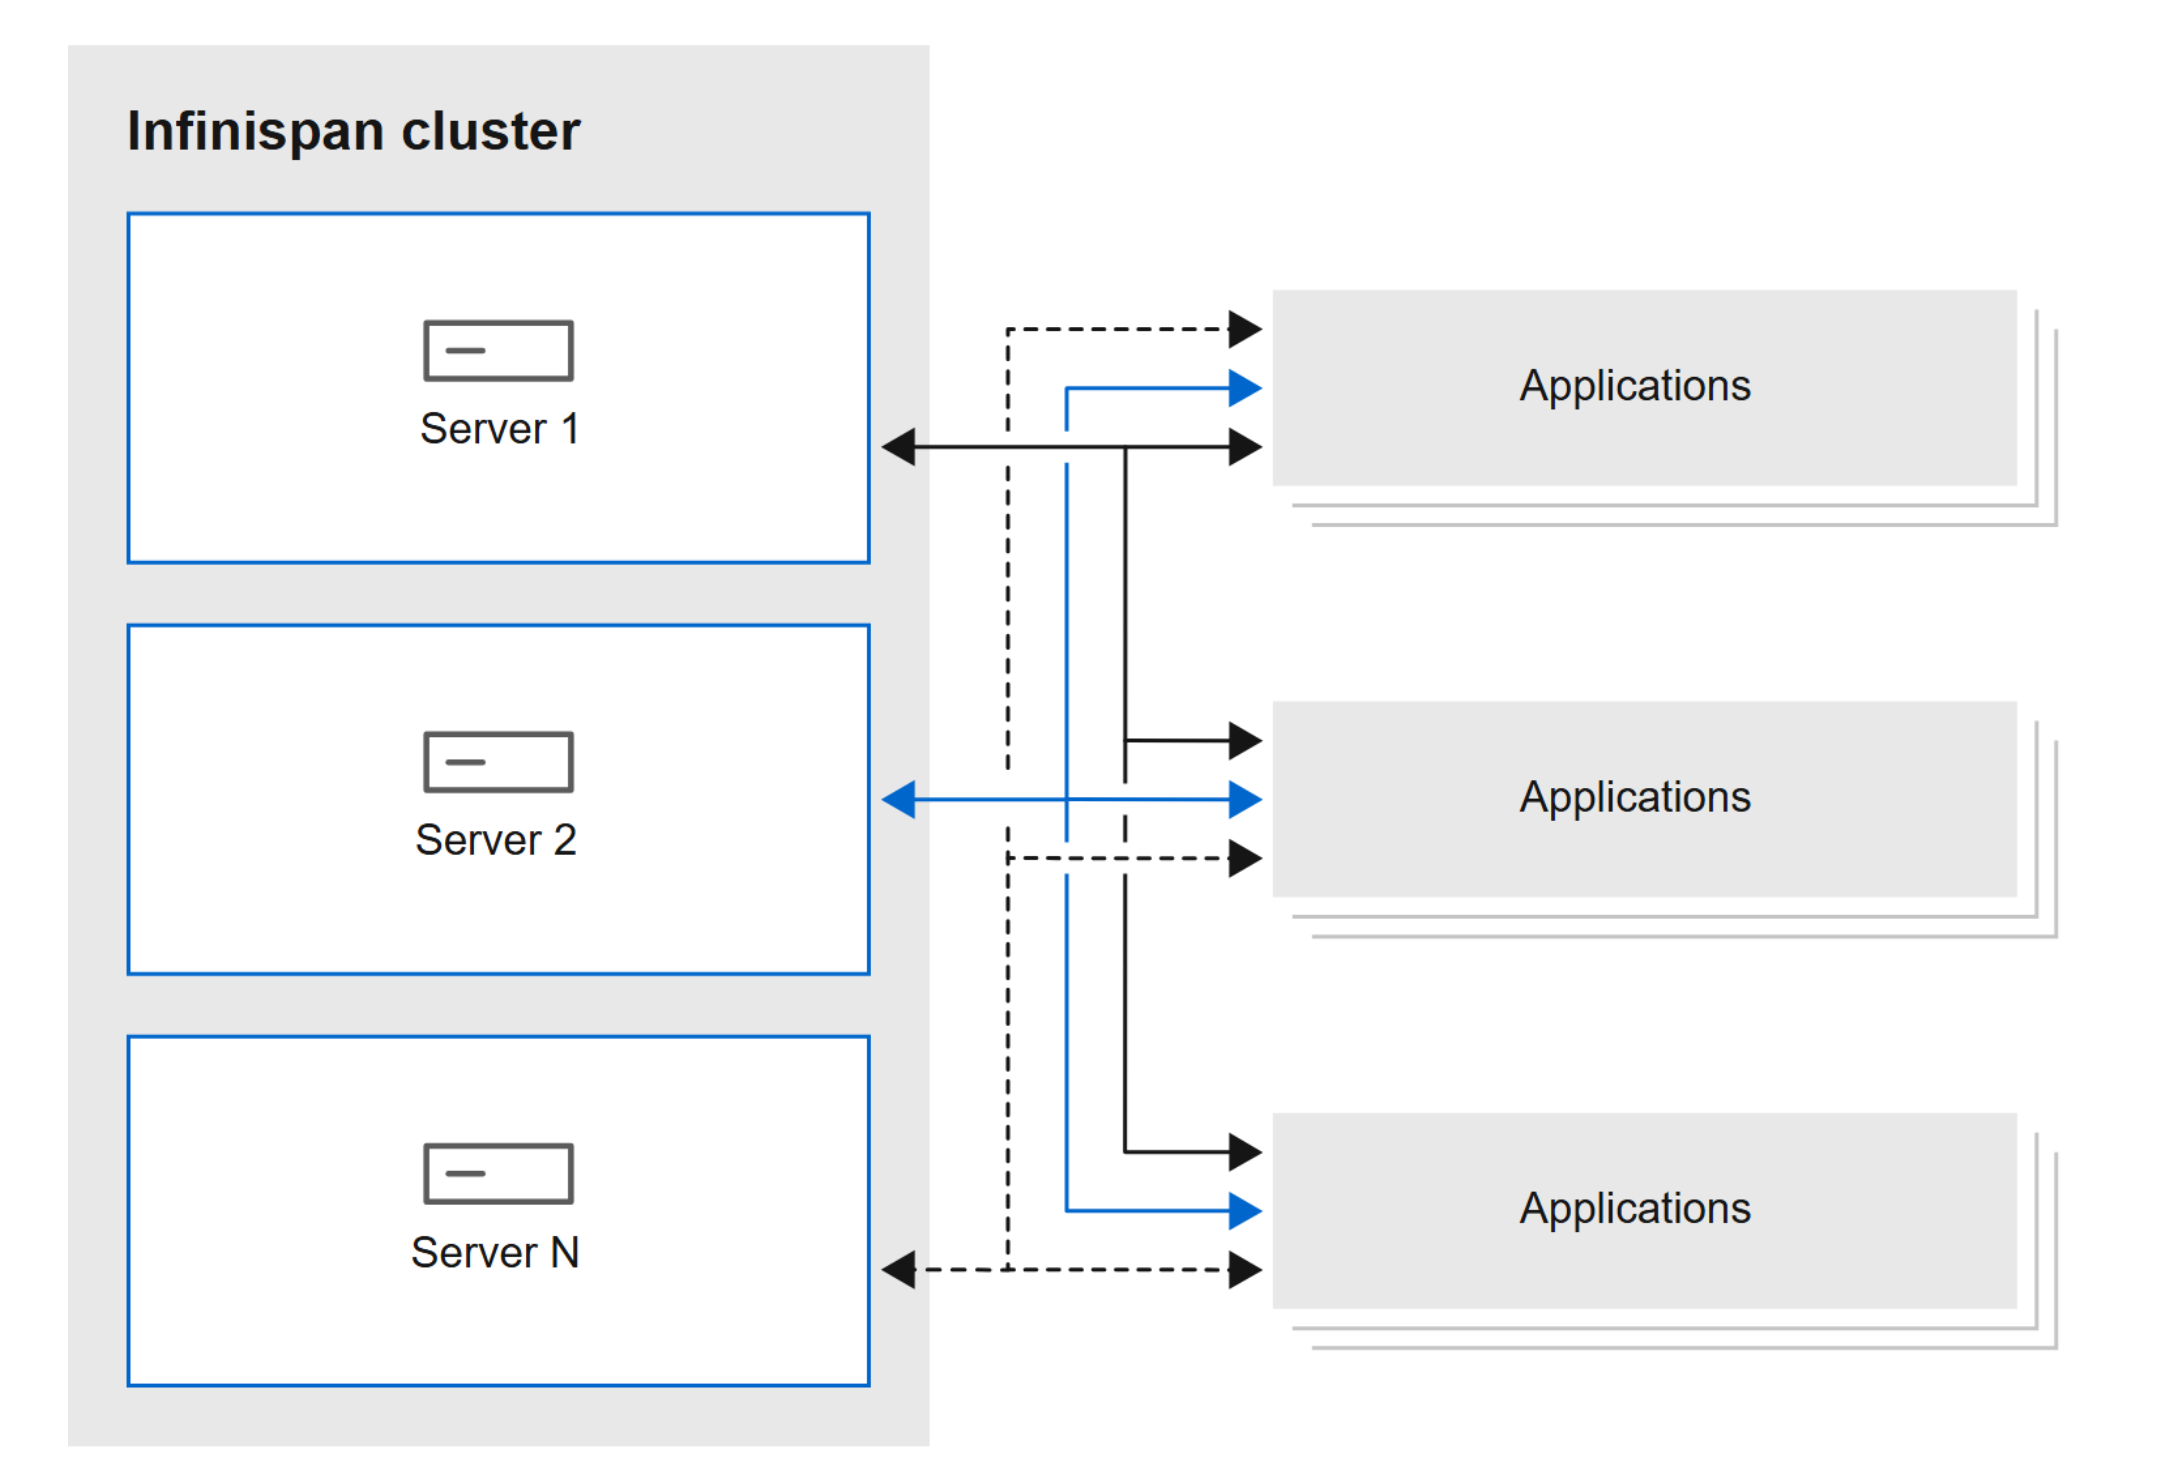
\includegraphics[width=0.85\textwidth]{figuras/infinispan-cluster.png}
\fonte{\citeonline{infinispan_tuning}}
\end{figure}

A distribuição de chaves entre nós segue o esquema de \emph{consistent hashing}, onde o conjunto de chaves é dividido em um número fixo de segmentos, definido por \texttt{numSegments}, e cada segmento é atribuído a uma lista de donos \revini{FUN-28}\cite[seção 2.2.2]{infinispan_configuring_15}\revfim{FUN-28}. \revini{FUN-29}O esquema padrão atribui as chaves aos mesmos nós em todos os \emph{caches}, desde que todos os \emph{caches} existam em todos os nós, ao custo de uma distribuição de carga levemente desigual \cite[seção 2.2.2]{infinispan_configuring_15}\revfim{FUN-29}; a variante ciente da topologia distribui as cópias por níveis topológicos como sites, racks e máquinas, para reduzir a chance de perda em falhas correlacionadas; e a variante de equilíbrio uniforme otimiza o balanceamento com a desvantagem de o resultado depender da ordem de entrada dos nós no \emph{cluster}. Quando a composição do \emph{cluster} muda, ocorre rebalanceamento, e segmentos são transferidos entre nós; durante a transição, mudanças de topologia podem causar repetições e mensagens adicionais para operações de leitura e escrita.

Nos modos \texttt{REPL\_SYNC} e \texttt{REPL\_ASYNC}, em contraste com a atribuição por segmentos própria dos modos distribuídos, cada nó mantém uma cópia completa de todas as entradas. A Figura~\ref{fig-datagrid-repl} representa esse comportamento em um \emph{data grid} replicado. Uma escrita submetida por um cliente, denotada \texttt{put()}, é aplicada em um nó e propagada aos demais pela replicação, assinalada como \texttt{REPL}, e cada nó atualiza os próprios índices locais a partir da atualização recebida. Uma consulta submetida por outro cliente, denotada \texttt{query}, é atendida localmente pelo nó que a recebe, pois todos os nós observam o mesmo conjunto de entradas depois de concluída a propagação. A figura torna visível o custo central da replicação assíncrona, dado que no intervalo entre a escrita local e a entrega da atualização aos demais nós as réplicas permanecem temporariamente divergentes.

\begin{figure}[htb]
\centering
\caption{Replicação de uma escrita entre os nós de um \emph{data grid}, com atualização dos índices por nó e leitura por consulta.}
\label{fig-datagrid-repl}
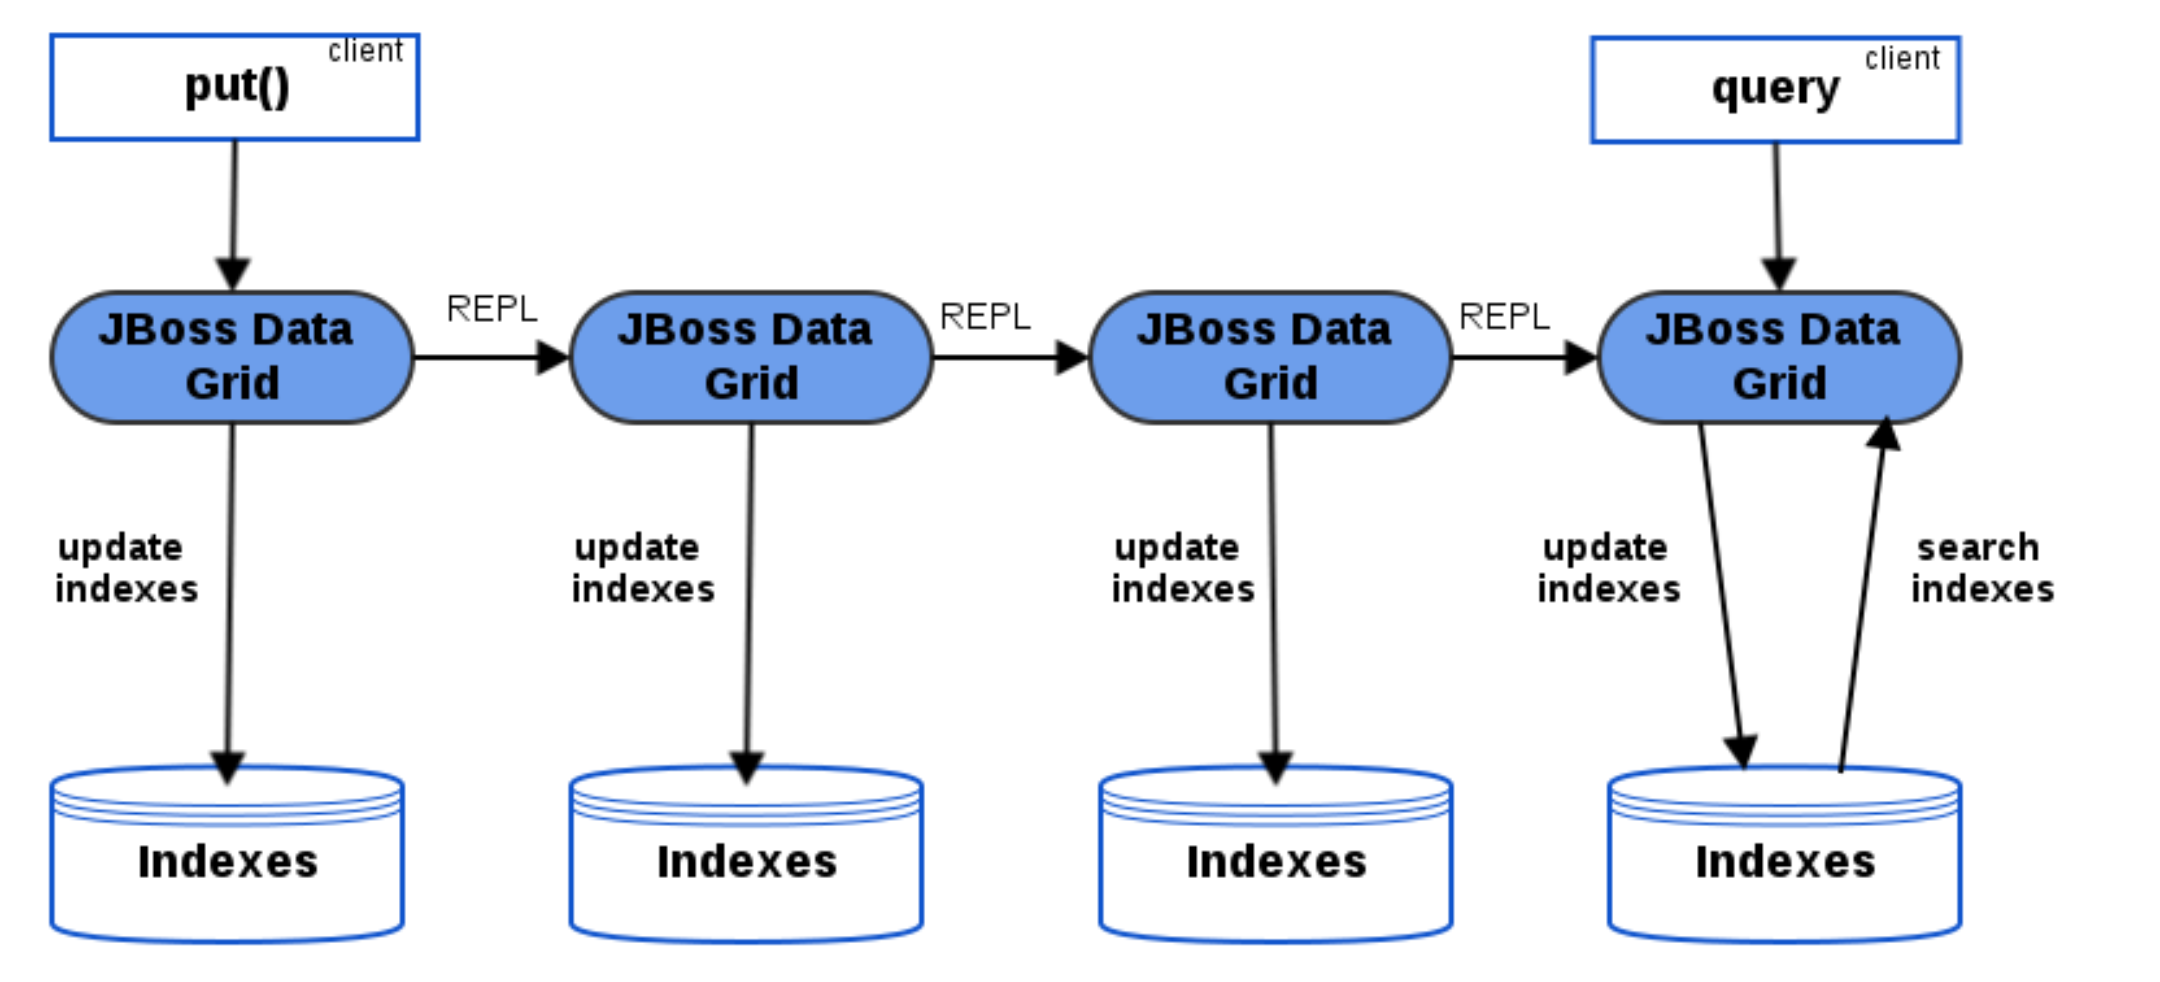
\includegraphics[width=0.95\textwidth]{figuras/datagrid-repl.png}
\fonte{\citeonline{redhat_datagrid_admin}}
\end{figure}

Para cenários multisite, a replicação \emph{cross-site}, ou seja, a replicação entre datacenters geograficamente distintos, permite cópias síncronas ou assíncronas entre \emph{clusters} separados \citep{infinispan_xsite}. A documentação registra duas regras importantes. A primeira é operacional: cópias assíncronas não adicionam latência às requisições do cliente, enquanto as síncronas introduzem o RTT entre sites em cada escrita, o que torna a opção assíncrona recomendada para configurações ativo-ativo em que dois sítios recebem escritas concorrentes. A segunda diz respeito à reconciliação: a detecção de conflitos por relógios vetoriais aciona políticas de resolução, com a política padrão usando comparação lexicográfica do nome do \emph{cluster}, e alternativas \texttt{ALWAYS\_REMOVE}, \texttt{PREFER\_NON\_NULL}, \texttt{PREFER\_NULL} ou implementação customizada pelo SPI \texttt{XSiteEntryMergePolicy}. A coleta de métricas operacionais segue documentação dedicada \citep{infinispan_metrics}: contadores por cache, indicadores de \emph{cluster}, sinais de \emph{cross-site}, latências médias e máximas, integração com JMX e exposição como Prometheus \citep{prometheus_docs}. Esses observáveis sustentam a instrumentação prevista para o controlador heurístico em etapa posterior.  Um ponto operacional ressaltado pela documentação merece registro: mesmo com replicação síncrona, caches distribuídos não são linearizáveis, dado que a escrita não é atômica entre os donos\revini{FUN-11} \cite[seção 2.2.1]{infinispan_configuring_15}\revfim{FUN-11}. Essa observação tem implicação direta sobre a formulação dos invariantes de sessão deste trabalho, dado que linearizabilidade não pode ser tomada como premissa nem no modo síncrono.

\section{Especificação formal e \emph{model checking}}
\label{sec-fund-formal}

A verificação por \emph{model checking} explora exaustivamente o espaço de estados de um modelo finito do sistema, com o objetivo de certificar a validade de propriedades declaradas ou produzir contraexemplos quando essas propriedades são violadas. \citet{yu_lamport_tla_modelchecking_1999} descrevem TLA+ como uma linguagem de especificação que combina a lógica temporal de ações TLA com lógica de primeira ordem completa e teoria dos conjuntos no estilo de Zermelo-Fraenkel. Uma especificação em TLA+ assume a forma canônica $\textit{Spec} \triangleq \textit{Init} \land \square [\textit{Next}]_v$, em que $\textit{Init}$ é um predicado sobre as variáveis $v$ que caracteriza os estados iniciais, $\textit{Next}$ é a relação de transição expressa como disjunção de ações, e $\square$ é o operador temporal que afirma que a fórmula a ele subordinada vale em todo estado da execução. Cada ação é um predicado sobre os valores das variáveis no estado corrente e no estado seguinte, denotadas $x$ e $x'$. Propriedades de invariância são fórmulas $\square \, P(v)$ que afirmam que todos os estados alcançáveis satisfazem $P$; propriedades temporais como $\square (P \Rightarrow \diamond Q)$ expressam restrições sobre sequências de estados e afirmam que todo $P$ é eventualmente seguido por um $Q$. O verificador TLC aceita um subconjunto de TLA+ adequado a descrições de sistemas reais, gera o grafo de estados acessíveis a partir dos estados iniciais \revini{FUN-30}por busca em largura\revfim{FUN-30}, mantém um conjunto de estados visitados por impressão digital de estado, e, quando encontra um estado que viola um invariante, retorna a sequência de transições que reproduz a violação. \citet{yu_lamport_tla_modelchecking_1999} \revini{FUN-31}registram o uso do TLC na especificação do protocolo de coerência de \emph{cache} de um novo multiprocessador da Compaq, com cerca de 1.800 linhas, na qual o verificador encontrou perto de duas dezenas de erros, dois deles presentes também na implementação em RTL, que foi corrigida \citep[seção 7]{yu_lamport_tla_modelchecking_1999}.\revfim{FUN-31}

A Figura~\ref{fig-tlc-estados} ilustra, em um exemplo mínimo com duas variáveis inteiras $x$ e $y$, a forma como o TLC percorre o espaço de estados. O estado inicial, definido por \textit{Init}, atribui o valor zero às duas variáveis. Cada aplicação da relação de transição \textit{Next} produz os estados sucessores admissíveis, e o não determinismo da relação faz um mesmo estado originar mais de um sucessor, como no ramo em que o estado com $x = 3$ dá origem a dois estados distintos após a segunda transição. O verificador repete esse passo sobre cada estado gerado e mantém o conjunto dos estados já visitados para não reexplorá-los. A verificação de um invariante avalia o predicado declarado em cada estado alcançado, e a primeira avaliação falsa interrompe a busca e devolve a sequência de transições que reproduz a violação.

\begin{figure}[htb]
\centering
\caption{Exploração do espaço de estados pelo verificador TLC, em que a relação de transição gera os estados sucessores a partir do estado inicial.}
\label{fig-tlc-estados}
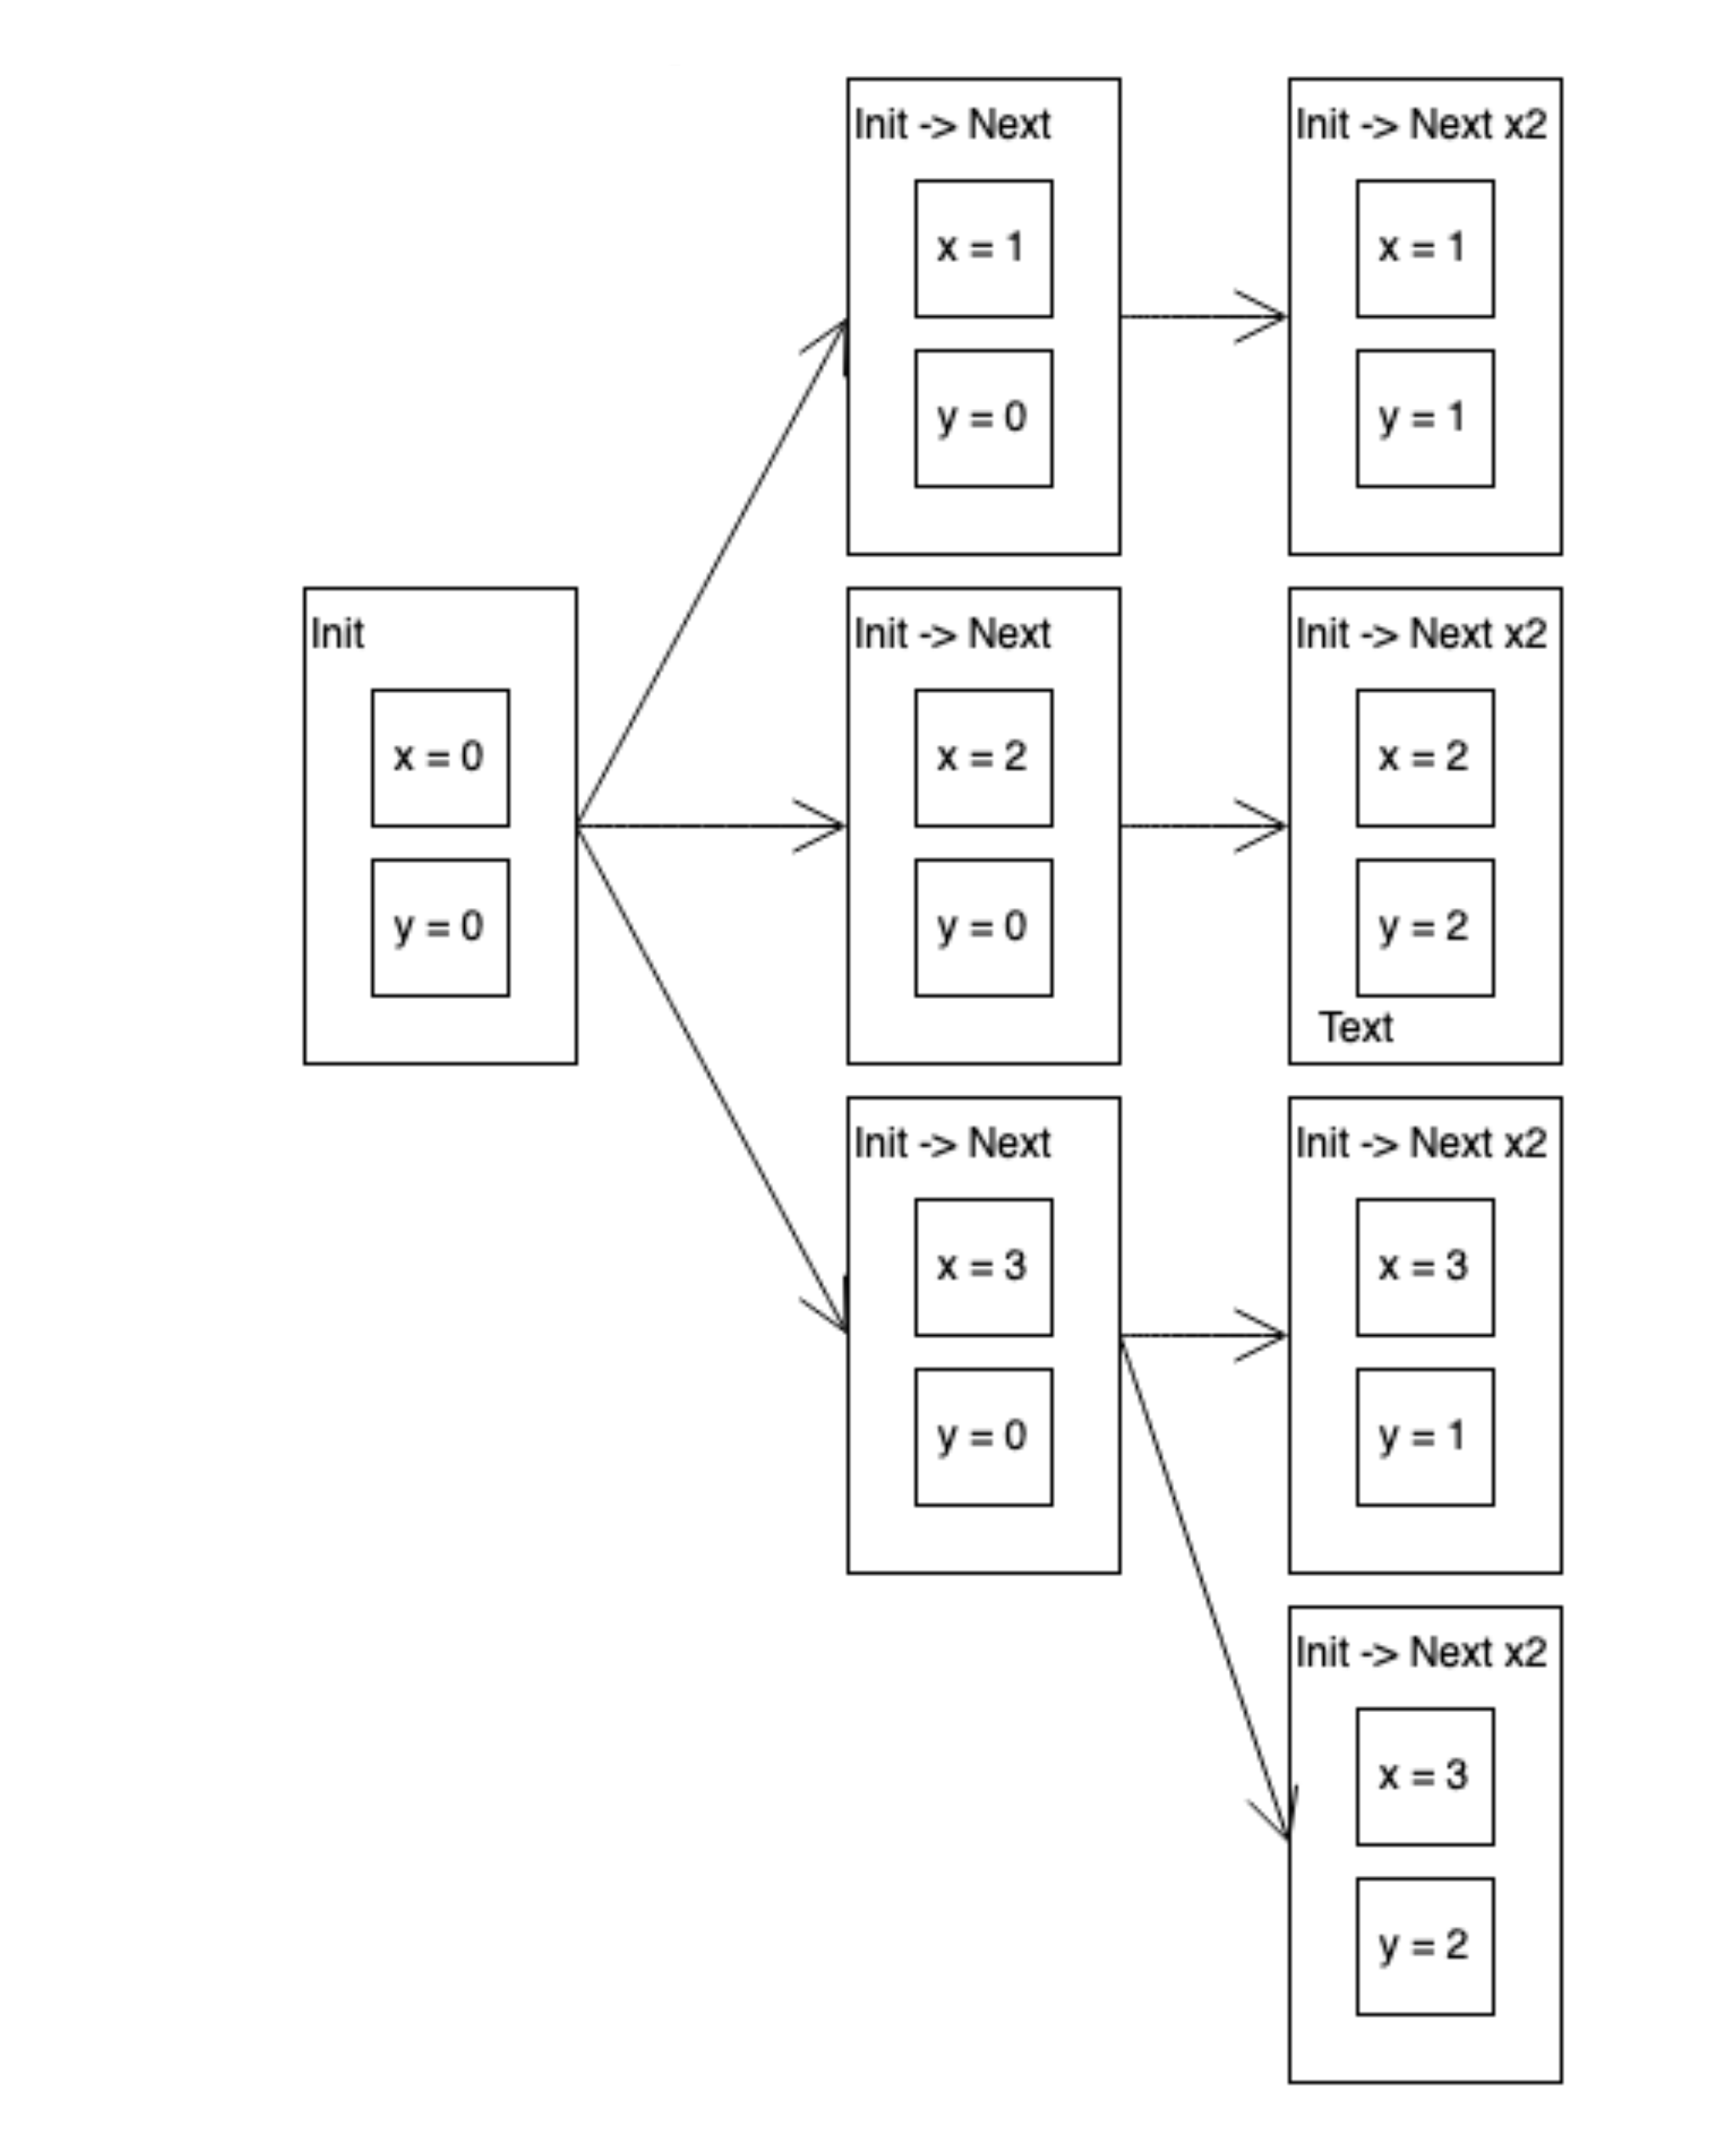
\includegraphics[width=0.62\textwidth]{figuras/tlc-estados.png}
\fonte{\citeonline{lee_tla_tlc_2021}}
\end{figure}

A representação eficiente do espaço de estados é o gargalo central da abordagem. \citet{yu_lamport_tla_modelchecking_1999} relatam estratégias para armazenar conjuntos de estados em disco e usar \revini{FUN-32}impressões digitais de 64 bits, únicas com alta probabilidade\revfim{FUN-32}, e essas opções determinam o tamanho dos modelos tratáveis. Em sistemas distribuídos, o espaço cresce com o número de nós, o tamanho da fila de mensagens em trânsito e a quantidade de tipos de evento, com explosão combinatória que motiva abstrações por simetria, por particionamento ou por redução parcial de ordem\revini{FUN-33} \citep{enea_must_2024}\revfim{FUN-33}. Daí a opção recorrente, no desenho de modelos formais para esses sistemas, por abstrações que mantenham a essência da concorrência sem replicar todos os detalhes da implementação. A aplicação industrial subsequente, com destaque para o registro de adoção pela Amazon Web Services, documenta a identificação de defeitos sutis em protocolos de replicação. \revini{FUN-12}\citet{newcombe_aws_formal_methods_2015}\revfim{FUN-12} relatam que a verificação formal encontrou, no projeto do DynamoDB, um defeito que poderia levar à perda de dados por meio de uma sequência de 35 passos envolvendo interações entre transações concorrentes, particionamento e recuperação, defeito que escapou a revisões extensivas de desenho, de código e a testes convencionais, e que motivou alteração no protocolo antes da implantação em produção.

A produção contemporânea estende a técnica em três direções. A primeira combina verificação formal e teste de implementações: um modelo formal guia testes incrementais sobre o sistema real, com o objetivo de aproximar o que foi verificado do que está executando, por instrumentação que mapeia transições do modelo a observações no código \citep{gao_mc_incremental_2025}. A segunda verifica diretamente protocolos distribuídos com semântica de mensagens assíncronas e falhas, em ferramentas projetadas para esse propósito; \revini{FUN-34}Must oferece uma interface de concorrência com vários modelos de comunicação, verifica os programas por redução parcial de ordem dinâmica e foi aplicada a sistemas de produção, como \emph{logs} replicados e protocolos de transação distribuída \citep{enea_must_2024}.\revfim{FUN-34} A terceira é a verificação probabilística de modelos: o resultado da análise é uma probabilidade de violação sob distribuições associadas a parâmetros do sistema, \revini{FUN-35}e aplica-se a decisões de escalonamento horizontal em bancos NoSQL ciente de custo \citep{naskos_probabilistic_mc_2017}\revfim{FUN-35}. A escolha da ferramenta para este trabalho, entre TLA+/TLC e as alternativas, fica detalhada e justificada na Seção~\ref{sec-escolha-ferramenta}.

\revini{FUN-13}A verificação exaustiva só é tratável com cardinalidades pequenas, e a pertinência desse recorte tem apoio empírico. \citet{yuan_simple_testing_2014}, ao analisar falhas reportadas em sistemas distribuídos de produção, constatam que \revini{FUN-36}98\% delas\revfim{FUN-36} se manifestam com três nós ou menos. A observação sustenta tanto os modelos com duas ou três réplicas verificados pelo TLC quanto o \emph{cluster} experimental de três nós, embora não garanta que todo defeito do protocolo apareça nessas cardinalidades.\revfim{FUN-13}

\section{Latência de cauda, objetivos de nível de serviço e observabilidade}
\label{sec-fund-slo}

A distribuição de latência de um serviço composto por muitos componentes tem cauda longa, e o impacto dessa cauda sobre o tempo total observado pelo usuário é desproporcional ao seu peso na distribuição. \citet{dean_barroso_tail_2013} ilustram o fenômeno com um caso em que a latência típica de uma requisição fica em torno de $10$ milissegundos, com 1\% das requisições demorando mais de $1$ segundo (cem vezes a típica). Em sistemas de \emph{fan-out}, em que uma requisição do usuário se decompõe em $n$ requisições independentes a componentes distintos e depende da resposta mais lenta, a probabilidade de pelo menos uma resposta cair na cauda cresce rapidamente com $n$: se a probabilidade de uma resposta individual ser lenta é $p = 0{,}01$, a probabilidade de pelo menos uma resposta lenta em $n = 100$ componentes é $1 - (1-p)^n \approx 0{,}63$, ou seja, 63\% das requisições do usuário tocam pelo menos uma resposta na cauda. \revini{FUN-37}As fontes de variabilidade apontadas pelos autores incluem disputa por recursos compartilhados na máquina e na rede, atividades de manutenção em segundo plano, como a coleta de lixo, filas em servidores e comutadores e mecanismos de economia de energia do \emph{hardware}.\revfim{FUN-37} Por isso, os percentis p95 e p99, e em sistemas críticos o p99,9, são as métricas primárias em vez da média. As técnicas de tolerância à cauda incluem requisições redundantes (\emph{hedged requests}), em que o cliente envia uma cópia secundária após $T$ milissegundos de espera, com $T$ tipicamente fixado no p95 esperado, e cancela a réplica que perde a corrida; e requisições atadas (\emph{tied requests}), em que servidores que recebem cópias se comunicam para cancelar a duplicata assim que um deles começa o atendimento. \revini{FUN-38}Esperar até o p95 limita a carga adicional das requisições redundantes a cerca de 5\%, e em um exemplo dos autores 2\% de requisições a mais reduziram o p99,9 de 1.800 para 74 milissegundos; nas requisições atadas, a sobrecarga medida em uso de disco ficou abaixo de 1\%.\revfim{FUN-38}

A formulação dessas metas como objetivos de nível de serviço segue prática consolidada \citep{google_sre_slo}. Um indicador de nível de serviço (SLI) é definido como uma medida quantitativa de algum aspecto do nível de serviço fornecido. Um objetivo de nível de serviço (SLO) é um valor-alvo, ou intervalo de valores, para o nível de serviço medido por um SLI, expresso como $\text{SLI} \le \text{alvo}$ ou $\text{limite inferior} \le \text{SLI} \le \text{limite superior}$; um exemplo prescrito pela literatura é ``99\% das chamadas de \texttt{Get} completam em menos de 100 milissegundos''. Um acordo de nível de serviço (SLA) é um contrato explícito ou implícito com os usuários, com consequências do cumprimento ou descumprimento dos SLO nele contidos. \revini{FUN-39}O orçamento de erros é a taxa com que os SLOs podem deixar de ser cumpridos, acompanhada diariamente ou semanalmente, e seu consumo funciona como entrada para decisões operacionais.\revfim{FUN-39} Sobre agregação, médias simples obscurecem detalhes importantes, e a combinação de mediana, p99 e p99,9 caracteriza a forma da distribuição com mais fidelidade do que qualquer estatística única.

A pesquisa específica em armazenamentos chave-valor estuda como reduzir a cauda de latência por agendamento de consultas, com algoritmos que tratam heterogeneidade de operações \citep{jaiman_tailx_2020, benmokhtar_taming_tail_2021}, e estende esse trabalho em versão expandida com avaliação ampla de cenários \citep{benmokhtar_scheduling_2024}. A observabilidade operacional encontra-se sistematizada em estudos sobre rastreamento e análise em microsserviços, que documentam práticas de instrumentação, retenção e análise de sinais sobre execuções distribuídas \citep{li_observability_2021}. No Infinispan, os contadores e indicadores publicados conforme a documentação de métricas dão acesso aos observáveis necessários para correlacionar variações de latência e eventos operacionais com violações de invariantes \citep{infinispan_metrics}.

\revini{FUN-14}\label{sec-fund-avaliacao}A avaliação experimental de sistemas computacionais precisa lidar com a variabilidade entre execuções. \citet{georges_jvm_statistics_2007} mostram que o desempenho de programas Java não é determinístico, por efeito de fatores como a compilação dinâmica, a coleta de lixo e o escalonamento de \emph{threads}, e que metodologias de avaliação sem rigor estatístico podem levar a conclusões enganosas. Para médias estimadas a partir de poucas execuções, o intervalo de confiança usa a distribuição $t$ de \citet{student_probable_error_1908}. \citet{hoefler_belli_benchmarking_2015} sistematizam regras para relatar resultados de desempenho, entre elas tratar a execução repetida como unidade de medida, reportar a variabilidade por intervalos de confiança e preferir procedimentos não paramétricos quando os dados não seguem distribuição normal. Para estatísticas sem distribuição amostral conhecida, como os percentis de latência, o \emph{bootstrap} aproxima essa distribuição por reamostragem dos dados observados, e o intervalo percentil toma os quantis da distribuição reamostrada \citep{efron_tibshirani_bootstrap_1993}. O teste de \citet{mann_whitney_1947} compara duas amostras sem supor normalidade e verifica se uma das variáveis tende a assumir valores maiores que a outra. Para proporções, \citet{brown_cai_dasgupta_binomial_2001} mostram que o intervalo padrão baseado na aproximação normal da binomial tem cobertura errática, que se afasta do nível nominal de modo irregular, o que recomenda cautela no uso dessa aproximação.\revfim{FUN-14}

\revini{FUN-15}Quando o mesmo pesquisador desenha, executa e analisa um experimento, decisões tomadas depois de ver os dados podem ser apresentadas, sem intenção, como previsões. \citet{nosek_preregistration_2018} defendem o pré-registro como resposta: hipóteses, desfechos e plano de análise são fixados antes da coleta, o que separa a análise confirmatória da exploratória.\revfim{FUN-15}

\revini{FUN-16}A estimativa de energia parte de modelos de potência por utilização. \citet{fan_power_provisioning_2007} observam que a potência de um servidor varia de forma aproximadamente linear com a utilização da CPU, o que permite estimá-la por $P(u) = P_\text{ocioso} + (P_\text{máx} - P_\text{ocioso}) \cdot u$, em que $u$ é a utilização. \citet{barroso_holzle_energy_proportional_2007} mostram que servidores consomem parcela elevada da potência de pico mesmo quando ociosos e passam a maior parte do tempo em utilização baixa ou moderada, de modo que a parcela ociosa pesa na energia por operação. Em máquinas virtuais, a potência não pode ser medida diretamente no \emph{hardware} e precisa ser estimada por modelos alimentados por contadores de uso de recursos \citep{kansal_vm_power_2010}. No Linux, a interface de grupos de controle versão 2 (cgroup v2) expõe o tempo de CPU acumulado por grupo de processos, o que permite atribuir o tempo de CPU a cada \emph{container} \citep{linux_cgroup_v2}.\revfim{FUN-16}

\section{Sistemas autoadaptativos e controle por realimentação}
\label{sec-fund-adapt}

Um sistema autoadaptativo monitora seu próprio comportamento, analisa desvios em relação a metas e atua sobre parâmetros configuráveis para retornar à região operacional. Em ambientes de nuvem, a literatura organiza essas atividades por meio de taxonomias e revisões que descrevem mecanismos de elasticidade sob a ótica da teoria de controle, com critérios como estabilidade, tempo de acomodação e prevenção de oscilação \citep{ullah_control_elasticity_2018}. Trabalhos de implementação demonstram autoescala em armazenamentos de nuvem hierárquicos \citep{wu_anna_autoscale_2020} e gestores proativos de elasticidade autotreinados \citep{liu_onlineelastman_2017}. Para o desenho de controladores adaptativos, a literatura discute mecanismos de garantia que combinam evidência empírica e propriedades formais \citep{gambi_assurance_selfadaptive_2013}, e propõe políticas de auto-gestão baseadas em objetivos de alto nível em sistemas distribuídos \citep{rosa_selfmgmt_2013}. \revini{FUN-17}A referência conceitual comum a esses trabalhos é o laço monitorar-analisar-planejar-executar sobre uma base de conhecimento (MAPE-K), do gerente autônomo descrito por \citeonline{kephart_chess_autonomic_2003}.\revfim{FUN-17}

O controlador previsto para etapa posterior deste trabalho é heurístico, com regras determinísticas e mecanismos de histerese para evitar oscilação, e atua sobre um conjunto finito de configurações pré-definidas.  A escolha do desenho heurístico, em lugar de soluções baseadas em aprendizado de máquina ou em controle ótimo, segue dois critérios. O primeiro é a auditabilidade das decisões: cada ação aplicada pelo controlador pode ser rastreada para a regra que a motivou, o que sustenta análise de causa raiz após qualquer ocorrência. O segundo é a tratabilidade formal: regras determinísticas com observáveis bem-definidos prestam-se à análise pelo modelo formal do trabalho, conforme delineado no Capítulo~\ref{cap-metodologia}. \revini{FUN-40}\citet{ullah_control_elasticity_2018} apontam que controladores de elasticidade precisam evitar oscilação e se acomodar rapidamente após perturbações, e três fenômenos operacionais merecem atenção.\revfim{FUN-40} O primeiro é a alternância rápida entre estados de configuração, que introduz instabilidade e impede que qualquer estado se mantenha por tempo suficiente para produzir efeito. O segundo é a sobre-resposta, em que a reação supera a correção necessária e leva o sistema a oscilar em torno do valor-alvo. O terceiro é o atraso de fase, em que a ação chega depois da janela em que produziria efeito. Regras com histerese e limites de taxa de mudança são respostas diretas a esses três fenômenos.

\section{Gerência de sessão como domínio}
\label{sec-fund-sessao}

A gerência de sessão constitui o estudo de caso do trabalho. O ciclo de vida de uma sessão compreende criação, validação, renovação, invalidação e bloqueio, sobre uma identidade autenticada. \revini{FUN-19}A literatura normativa estabelece propriedades que esse ciclo deve satisfazer. A publicação SP 800-63B-4 do NIST, que substituiu a versão de 2017, define níveis de garantia do autenticador com prazos de reautenticação próprios de cada nível, trata da gerência de sessão em seção normativa, na qual exige que os segredos de sessão sejam invalidados no \emph{logout}, e exige a limitação do número de tentativas de autenticação malsucedidas, o chamado \emph{rate limiting} \cite[seções 2, 3.2.2 e 5]{nist_sp_800_63b4_2025}. Essas duas exigências fundamentam, respectivamente, a irreversibilidade da invalidação e o par formado pelo contador de tentativas e pelo bloqueio da identidade, objetos dos invariantes deste trabalho.\revfim{FUN-19}

A Figura~\ref{fig-sessao-ciclo} sintetiza o percurso de uma sessão autenticada quando o estado é externalizado para um repositório compartilhado. O usuário inicia o fluxo ao submeter credenciais em uma operação de \emph{login}, que o serviço de \emph{backend} autentica; confirmada a identidade, o serviço cria a sessão, registra-a no repositório de sessões e devolve ao cliente um \emph{cookie} que carrega apenas o identificador da sessão. Nas requisições seguintes, o cliente reapresenta esse \emph{cookie}, e o serviço valida a sessão por consulta ao repositório antes de produzir a resposta. A figura evidencia que a correção observada pelo usuário depende do estado mantido no repositório, e essa camada, quando replicada de forma assíncrona, expõe os invariantes de sessão às condições de falha tratadas neste trabalho.

\begin{figure}[htb]
\centering
\caption{Ciclo de vida de uma sessão autenticada com estado externalizado em repositório de sessões compartilhado.}
\label{fig-sessao-ciclo}
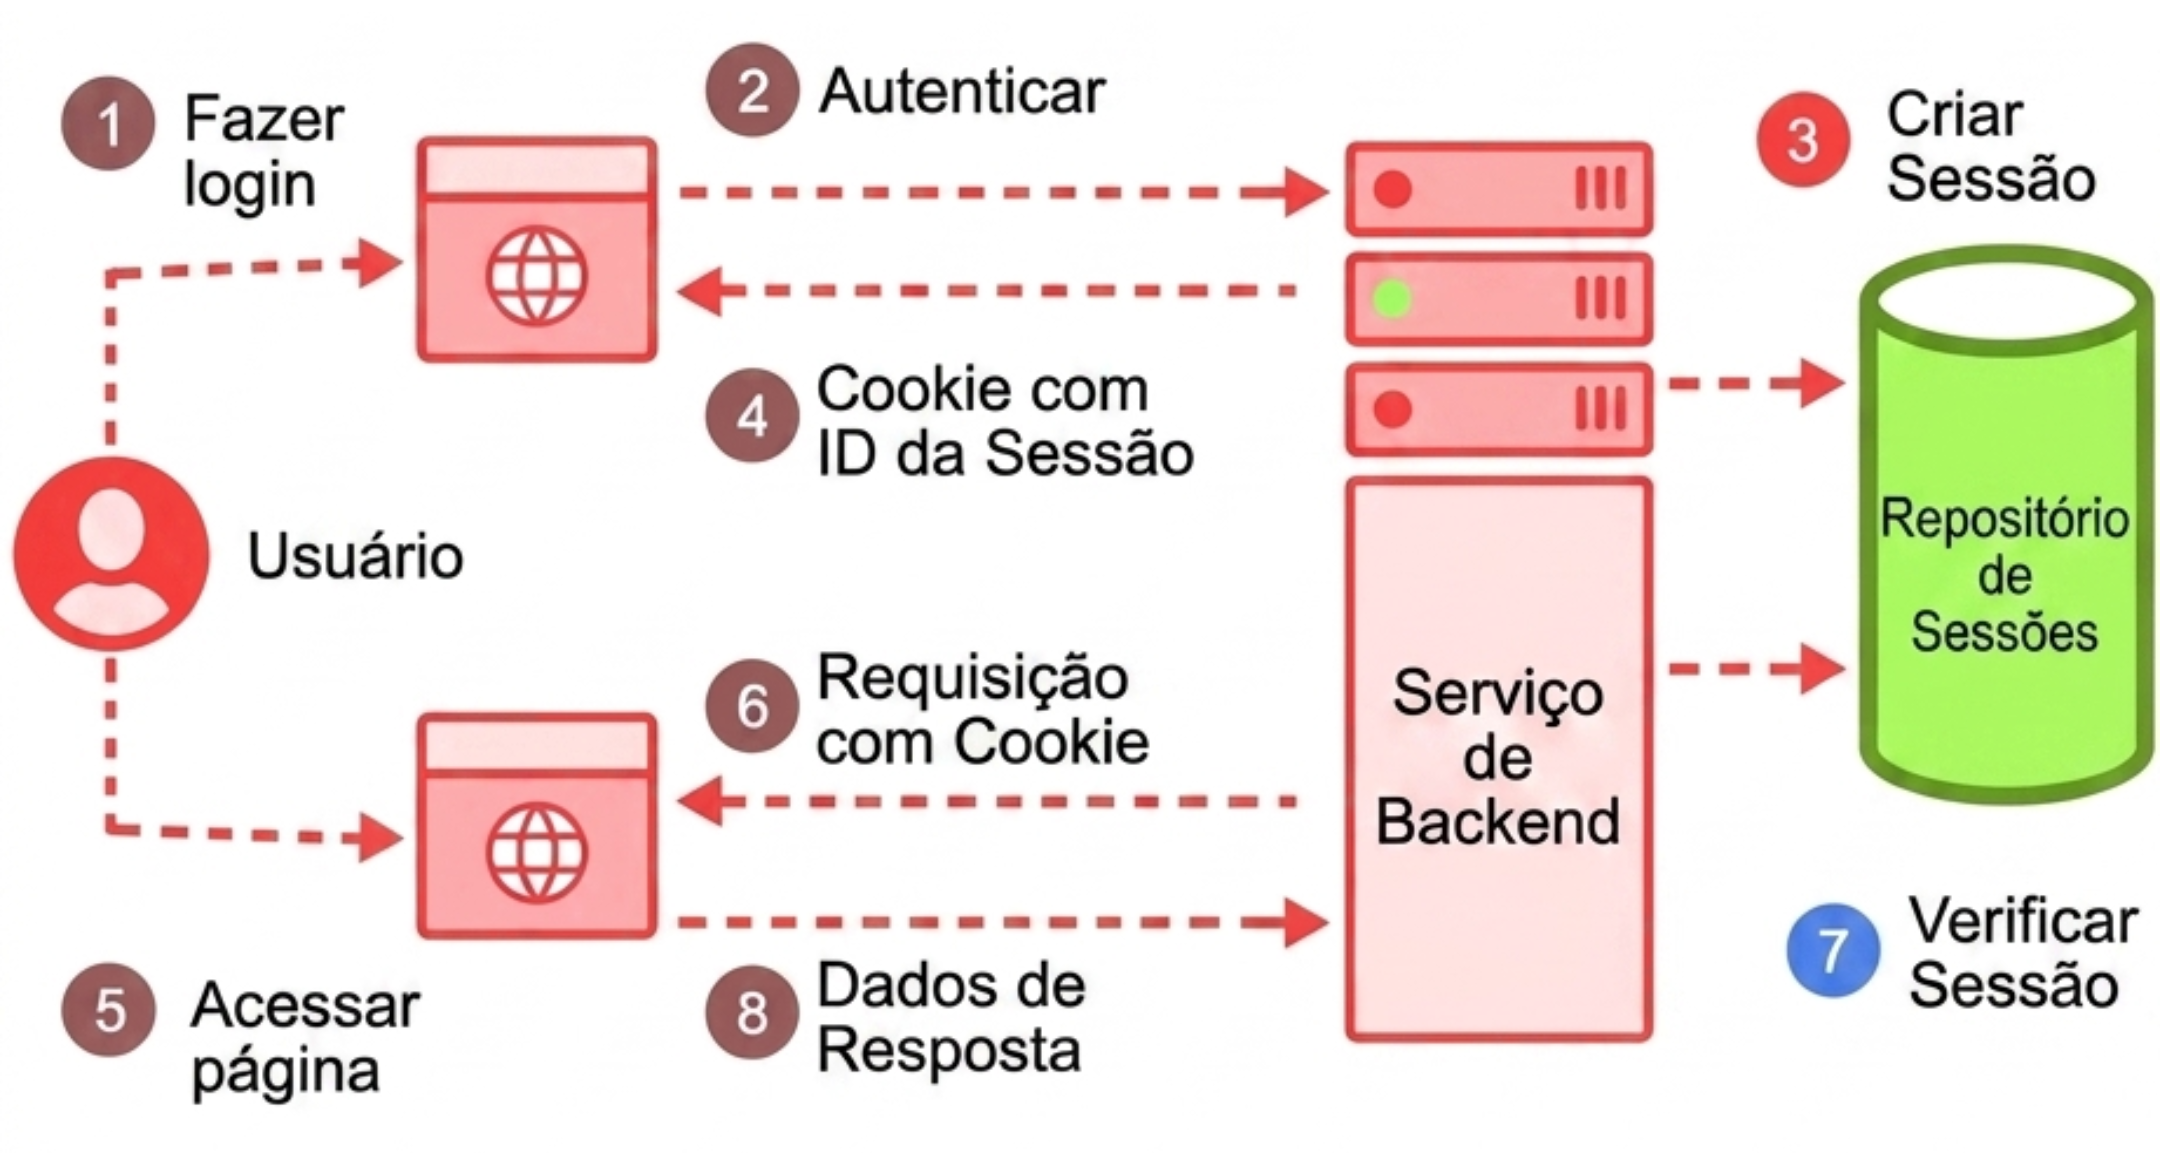
\includegraphics[width=0.9\textwidth]{figuras/sessao-ciclo.png}
\fonte{O autor}
\end{figure}

O \emph{OWASP Session Management Cheat Sheet} \citep{owasp_session_mgmt_cheatsheet} traduz essas exigências em requisitos operacionais sobre identificadores e atributos de sessão. O identificador de sessão deve ter pelo menos 64 bits de entropia, gerados por um gerador pseudoaleatório criptograficamente seguro, e deve evitar conteúdo significativo, ou seja, qualquer informação que permita a um observador deduzir o estado da sessão. Sobre o tempo de vida, três mecanismos complementares são prescritos: o tempo-limite absoluto define o tempo máximo de existência da sessão; o tempo-limite por inatividade encerra a sessão após inatividade; o tempo-limite de renovação rotaciona o identificador em intervalos regulares para reduzir a janela de exploração de identificadores capturados. A invalidação deve ser feita no servidor e no cliente, e o identificador deve ser regenerado após qualquer mudança de privilégio, em particular após a autenticação, para impedir ataques de fixação de sessão (\emph{session fixation}). Os atributos do \emph{cookie} devem incluir \texttt{Secure}, \texttt{HttpOnly}, \texttt{SameSite} e o prefixo \texttt{\_\_Host-}, para mitigar exposição em canal não seguro, acesso por código executado no cliente e envio em requisições de origem distinta.

\revini{FUN-41}Externalizar o estado de sessão em um IMDG ou armazenamento chave-valor aplica essa separação entre computação sem estado e armazenamento com estado \citep{armbrust_cloud_2010}: múltiplas instâncias servem requisições de um mesmo cliente sob balanceamento de carga.\revfim{FUN-41} A externalização desacopla o estado do nó que atende à requisição, com o ganho de continuidade em \emph{failover} e o custo da exposição aos efeitos da replicação assíncrona descritos na Seção~\ref{sec-fund-distrib}. A combinação dessas duas camadas, exigências normativas e operacionais, justifica a escolha de irreversibilidade de invalidação, consistência de bloqueio e monotonicidade de contadores como invariantes alvo deste trabalho.

\chapter{Metodologia}
\label{cap-metodologia}
% Capítulo 3, Metodologia

\label{sec-tipo-pesquisa}

Este é um trabalho de pesquisa aplicada, de natureza experimental e quantitativa, com objetivos exploratórios e descritivos, e segue estratégia metodológica mista, organizada em duas linhas de trabalho. A primeira aplica um mapeamento sistemático da literatura \citep{petersen_mapping_2008} para identificar e classificar abordagens relacionadas a invariantes de estado de sessão, replicação assíncrona, tolerância a falhas, verificação formal por \emph{model checking} e mecanismos de decisão em sistemas distribuídos. A segunda é de pesquisa de projeto: o trabalho constrói e avalia, sob cenários parametrizados de falha, um conjunto de artefatos com recorte derivado dos achados da linha de mapeamento; os artefatos previstos são o modelo formal, o programa de carga instrumentado, o ambiente experimental em \emph{cluster} Infinispan e, em etapa posterior, o controlador heurístico. O relato dos resultados do mapeamento adota elementos do PRISMA 2020 \citep{prisma_2020}, em particular o fluxograma de seleção e a contabilização de itens por etapa. O guia em língua portuguesa de \citet{neiva_silva_revisao_sistematica_2016} apoia a operação do mapeamento. Por se tratar de um trabalho dividido em duas etapas, Trabalho de Conclusão de Curso~I e Trabalho de Conclusão de Curso~II, o presente texto reporta o protocolo, a execução inicial do mapeamento e os resultados parciais relativos à primeira etapa. 

\section{Mapeamento sistemático da literatura}
\label{sec-ms}
\revini{MET-02}\label{ap-protocolo-ms}\revfim{MET-02}

O mapeamento sistemático segue a sequência canônica proposta por \citet{petersen_mapping_2008}: define as questões de mapeamento, conduz a busca em bases bibliográficas, triagem os resultados por título e resumo, \revini{MET-55}classifica os trabalhos por palavras-chave extraídas dos resumos, recorrendo a outras partes do texto quando o resumo não basta, e, por fim, extrai e sintetiza os dados\revfim{MET-55}, e produz um esquema de classificação acompanhado de uma síntese descritiva. Esta seção sintetiza os elementos principais e relata a execução até a triagem inicial, correspondente ao escopo do presente Trabalho de Conclusão de Curso~I.

\section*{Pergunta central e questões de mapeamento}
\label{ap-questoes}

A pergunta central de pesquisa, formulada na Seção~\ref{sec-problema}, desdobra-se em sete questões de mapeamento. As questões investigam, respectivamente, quais invariantes de domínio do estado de sessão são tratados na literatura, quais modelos de falha são assumidos, quais mecanismos de replicação e reconciliação são empregados, quais abordagens e ferramentas de verificação formal são aplicadas, quais métricas e indicadores operacionais são reportados, quais mecanismos de decisão e adaptação são propostos, e quais plataformas e sistemas-alvo aparecem nos estudos empíricos. Cada questão está associada a um ou mais eixos temáticos do trabalho, conforme detalhado na Tabela~\ref{qd-qm}.

\begin{table}[h]
\captionsetup{type=table, name=Tabela}
\caption{Questões de mapeamento e eixos temáticos correspondentes}
\centering
\begin{tabular}{p{2.3cm}p{9cm}p{2.6cm}}
\hline
\textbf{Identificador} & \textbf{Questão de mapeamento} & \textbf{Eixos} \\
\hline
QM1 & Quais invariantes de domínio do estado de sessão são tratados na literatura? & sessão, replicação \\
QM2 & Quais modelos de falha são assumidos pelos trabalhos? & falhas, replicação \\
QM3 & Quais mecanismos de replicação e reconciliação são empregados? & replicação, IMDG \\
QM4 & Quais abordagens e ferramentas de verificação formal são aplicadas? & métodos formais \\
QM5 & Quais métricas e indicadores operacionais são reportados? & SLO, latência, observabilidade \\
QM6 & Quais mecanismos de decisão e adaptação são propostos? & autoadaptativo, controle \\
QM7 & Quais plataformas e sistemas-alvo são objeto dos estudos empíricos? & IMDG \\
\hline
\end{tabular}
\fonte{O autor}
\label{qd-qm}
\end{table}

\label{ap-bases-strings}A busca é executada nas bases ACM Digital Library, IEEE Xplore, Scopus e SpringerLink, escolhidas por reunirem as principais editoras e indexadores em Ciência da Computação. Conforme descrito na Seção~\ref{ap-selecao-validade}, a execução inicial empregou o agregador OpenAlex como porta única de acesso, e essa decisão deve ser complementada por execução manual via Portal de Periódicos CAPES na versão definitiva do protocolo. 

A pesquisa emprega seis \emph{strings} complementares, denotadas S1 a S6, organizadas por foco temático. Cada \emph{string} combina cláusulas \emph{OR} de termos-foco com cláusulas \emph{AND} de filtros transversais, e resulta de duas rodadas de calibração contra um conjunto-semente nomeado de referências-âncora. As versões finais das \emph{strings} são as seguintes:

\begin{itemize}[leftmargin=*]
    \item \textbf{S1, replicação, consistência e IMDG:} \texttt{((''in-memory data grid'' OR IMDG OR ''distributed cache'' OR ''key-value store'' OR ''session state'' OR ''session management'' OR ''distributed storage'' OR ''consistent hashing'' OR ''rebalancing'' OR ''state transfer'') AND (''consistency'' OR ''invariant'' OR ''convergence'' OR ''reconciliation'' OR ''replication'' OR ''CRDT'' OR ''eventual consistency'' OR ''session consistency''))}

    \item \textbf{S2, métodos formais aplicados a sistemas distribuídos:} \texttt{((''model checking'' OR ''formal verification'' OR ''formal specification'' OR ''temporal logic'' OR ''TLA+'' OR ''TLA'' OR Alloy OR SPIN OR Coq OR Isabelle OR ''bounded model checking'' OR ''probabilistic model checking'' OR ''theorem proving'') AND (''distributed'' OR ''replicated'' OR ''replication'' OR ''consistency'' OR ''concurrent'' OR ''protocol'' OR ''fault'' OR ''cache'' OR ''data grid''))}

    \item \textbf{S3, SLO, latência de cauda e observabilidade:} \texttt{((''SLO'' OR ''service level objective'' OR ''service level agreement'' OR ''tail latency'' OR ''p95'' OR ''p99'' OR ''percentile latency'' OR observability OR ''distributed tracing'' OR ''system monitoring'') AND (''distributed'' OR ''data grid'' OR ''cache'' OR ''key-value'' OR ''replicated'' OR ''scale'' OR ''latency''))}

    \item \textbf{S4, sistemas autoadaptativos e controle:} \texttt{((''self-adaptive'' OR autonomic OR ''MAPE-K'' OR ''feedback control'' OR ''control theory'' OR ''autoscaling'' OR ''auto-scaling'' OR ''autoscaler'' OR elasticity OR ''self-healing'' OR ''self-managing'' OR ''self-tuning'' OR ''adaptive control'') AND (''distributed'' OR ''cloud'' OR ''data grid'' OR ''key-value'' OR ''cache'' OR ''replicated'' OR ''fault'' OR ''service'' OR ''storage''))}

    \item \textbf{S5, fundamentos teóricos:} \texttt{((''consensus'' OR ''agreement protocol'' OR ''atomic broadcast'' OR ''linearizability'' OR ''failure detector'' OR ''impossibility'' OR ''network partition'' OR ''CAP theorem'' OR Byzantine OR Paxos OR Raft OR ''state machine replication'' OR ''vector clocks'' OR ''logical clocks'') AND (''distributed'' OR ''asynchronous'' OR ''fault-tolerant'' OR ''fault tolerance'' OR ''process'' OR ''replicat*''))}

    \item \textbf{S6, sessão como domínio:} \texttt{((''session management'' OR ''session state'' OR ''session invariant'' OR ''session lifecycle'' OR ''session token'' OR ''user session'' OR ''authentication state'' OR ''session fixation'' OR ''session hijacking'') AND (''distributed'' OR ''cluster'' OR ''replicat*'' OR ''cache'' OR ''data grid'' OR ''in-memory'' OR ''stateful'' OR ''security''))}
\end{itemize}

\section*{Critérios de inclusão e exclusão}
\label{ap-criterios}

Os critérios de inclusão filtram positivamente os trabalhos a considerar e são cinco. CI1 admite trabalho revisado por pares, obra clássica ou seminal, ou documentação técnica oficial. CI2 exige texto completo acessível. CI3 restringe os idiomas a português ou inglês. CI4 requer que o trabalho aborde, de modo substancial, pelo menos uma das questões de mapeamento. CI5 exige que o estudo trate como tema central sistemas distribuídos, replicação, consistência, falhas, verificação formal, observabilidade, controle adaptativo ou gerência de sessão.

Os critérios de exclusão definem motivos de remoção e são sete. CE1 elimina trabalhos com apenas resumo disponível. CE2 elimina duplicatas, mantida a versão mais completa do mesmo trabalho. CE3 elimina documentos técnicos comerciais sem revisão por pares e sem conteúdo técnico verificável. CE4 elimina trabalhos cujo foco está fora dos eixos relevantes. CE5 elimina idiomas distintos dos aceitos. CE6 elimina fontes sem revisão por pares quando usadas como base teórica principal; relatórios técnicos do tipo \emph{Jepsen} são admitidos apenas como literatura cinza de apoio empírico. \revini{MET-56}CE7 elimina itens anteriores a 1985, ano do resultado de impossibilidade do consenso assíncrono \citep{fischer_lynch_paterson_flp_1985}, ressalvada\revfim{MET-56} a manutenção dos estudos seminais desse período pela cláusula CI1. Pela cláusula de inclusão, mantêm-se os estudos seminais anteriores a 1985, ano do resultado de impossibilidade do consenso assíncrono \citep{fischer_lynch_paterson_flp_1985}.

\section*{Esquema de extração e classificação}
\label{ap-extracao}

Cada estudo primário incluído é caracterizado pelas oito dimensões a seguir, com as categorias previstas registradas para cada uma. As categorias podem ser refinadas após a etapa de leitura completa, caso achados recorrentes não previstos justifiquem o ajuste.

\begin{description}[leftmargin=*, style=nextline]
    \item[D1, modelo de consistência alvo:] forte; sequencial; causal; sessão; eventual; consistência eventual forte (CRDT); quórum.
    \item[D2, modelo de falhas assumido:] parada silenciosa; parada com recuperação; omissão; particionamento; bizantino; misto; não especificado.
    \item[D3, mecanismo de replicação e reconciliação:] síncrona com quórum; assíncrona com gravação por último escritor; assíncrona com resolução pela aplicação; CRDT; relógios vetoriais; consenso (Paxos, Raft); replicação por máquina de estado.
    \item[D4, abordagem ou ferramenta formal:] TLA+ com TLC; Alloy; SPIN; Coq; Isabelle; verificação probabilística de modelos; verificação limitada de modelos; sem método formal.
    \item[D5, validação empírica realizada:] em IMDG identificado; em outro sistema; em simulação; não-empírico.
    \item[D6, domínio de aplicação:] sessão ou autenticação; chave-valor genérico; banco de dados distribuído; mensageria; cache de aplicação; outro.
    \item[D7, métricas reportadas:] latência média ou de cauda (p95, p99); vazão; taxa de violação; tempo de recuperação; tempo de convergência; consumo de recursos; outras.
    \item[D8, tipo de mecanismo adaptativo:] nenhum; estático configurável; heurístico baseado em regras; MAPE-K; controle de realimentação clássico; aprendizado de máquina.
\end{description}

\section*{Procedimento de seleção e ameaças à validade}
\label{ap-selecao-validade}
\label{sec-ms-execucao}

O procedimento de seleção compreende identificação, triagem por título e resumo, e elegibilidade por leitura completa. \revini{MET-04}A identificação registra, por base, a \emph{string} aplicada, a data de execução e a quantidade de itens retornados. A triagem por título e resumo aplica os critérios de exclusão imediatamente verificáveis. A elegibilidade aplica a leitura completa, com registro do motivo de cada exclusão.\revfim{MET-04} Os números obtidos em cada etapa são reportados conforme o padrão PRISMA 2020 \citep{prisma_2020}. A execução inicial do mapeamento, correspondente às semanas 3 e 4 do cronograma do Trabalho de Conclusão de Curso~I, foi conduzida em 13 de maio de 2026 e utilizou o agregador OpenAlex como porta única de acesso às bases declaradas, em razão de restrições de acesso programático aos portais. Essa decisão é registrada como limitação metodológica do mapeamento sistemático. A Tabela~\ref{qd-prisma} sintetiza o fluxo nas três primeiras categorias e registra a etapa de Inclusão como em curso, dado que a classificação final dos estudos primários selecionados integra o Trabalho de Conclusão de Curso~II.

\begin{table}[h]
\captionsetup{type=table, name=Tabela}
\caption{Síntese do fluxo PRISMA 2020 do mapeamento sistemático até a etapa atual}
\centering
\begin{tabular}{p{8cm}r}
\hline
\textbf{Etapa PRISMA e subetapa} & \textbf{Quantidade de itens} \\
\hline
Identificação: itens recuperados pela união das \emph{strings} S1 a S6 & 8.669 \\
Identificação: itens removidos por duplicidade por DOI ou identificador & 1.586 \\
Triagem: itens em triagem após deduplicação & 7.083 \\
Triagem: itens aceitos por filtros básicos (tipo, idioma, ano) & 6.590 \\
Triagem: itens adicionados pelo conjunto-semente de calibração & 8 \\
Triagem: itens aceitos por título e resumo & 2.536 \\
Elegibilidade: itens selecionados para leitura completa & 165 \\
Inclusão: itens classificados nas oito dimensões D1 a D8 & em curso \\
\hline
\end{tabular}
\fonte{O autor}
\label{qd-prisma}
\label{tab-ms-execucao}
\end{table}

O relato do processo de seleção adota o modelo de fluxograma do PRISMA 2020, reproduzido na Figura~\ref{fig-prisma}, que organiza o fluxo de itens em três blocos sucessivos, denominados \emph{Identification}, \emph{Screening} e \emph{Included}, e reserva em cada etapa um campo para a contagem de registros e para os motivos de remoção. A figura apresenta o arcabouço em sua forma de modelo, com os campos de contagem ainda não preenchidos, dado que a versão povoada com os números de cada etapa, a contagem da etapa de Inclusão e o detalhamento dos motivos de exclusão (CE1 a CE7) por etapa será apresentada na monografia final, após a classificação integral dos 165 estudos primários selecionados. Os quantitativos já apurados até a etapa atual constam da Tabela~\ref{qd-prisma}.



\begin{figure}[htb]
\centering
\caption{Modelo de fluxograma PRISMA 2020 para o relato do processo de seleção de estudos.}
\label{fig-prisma}
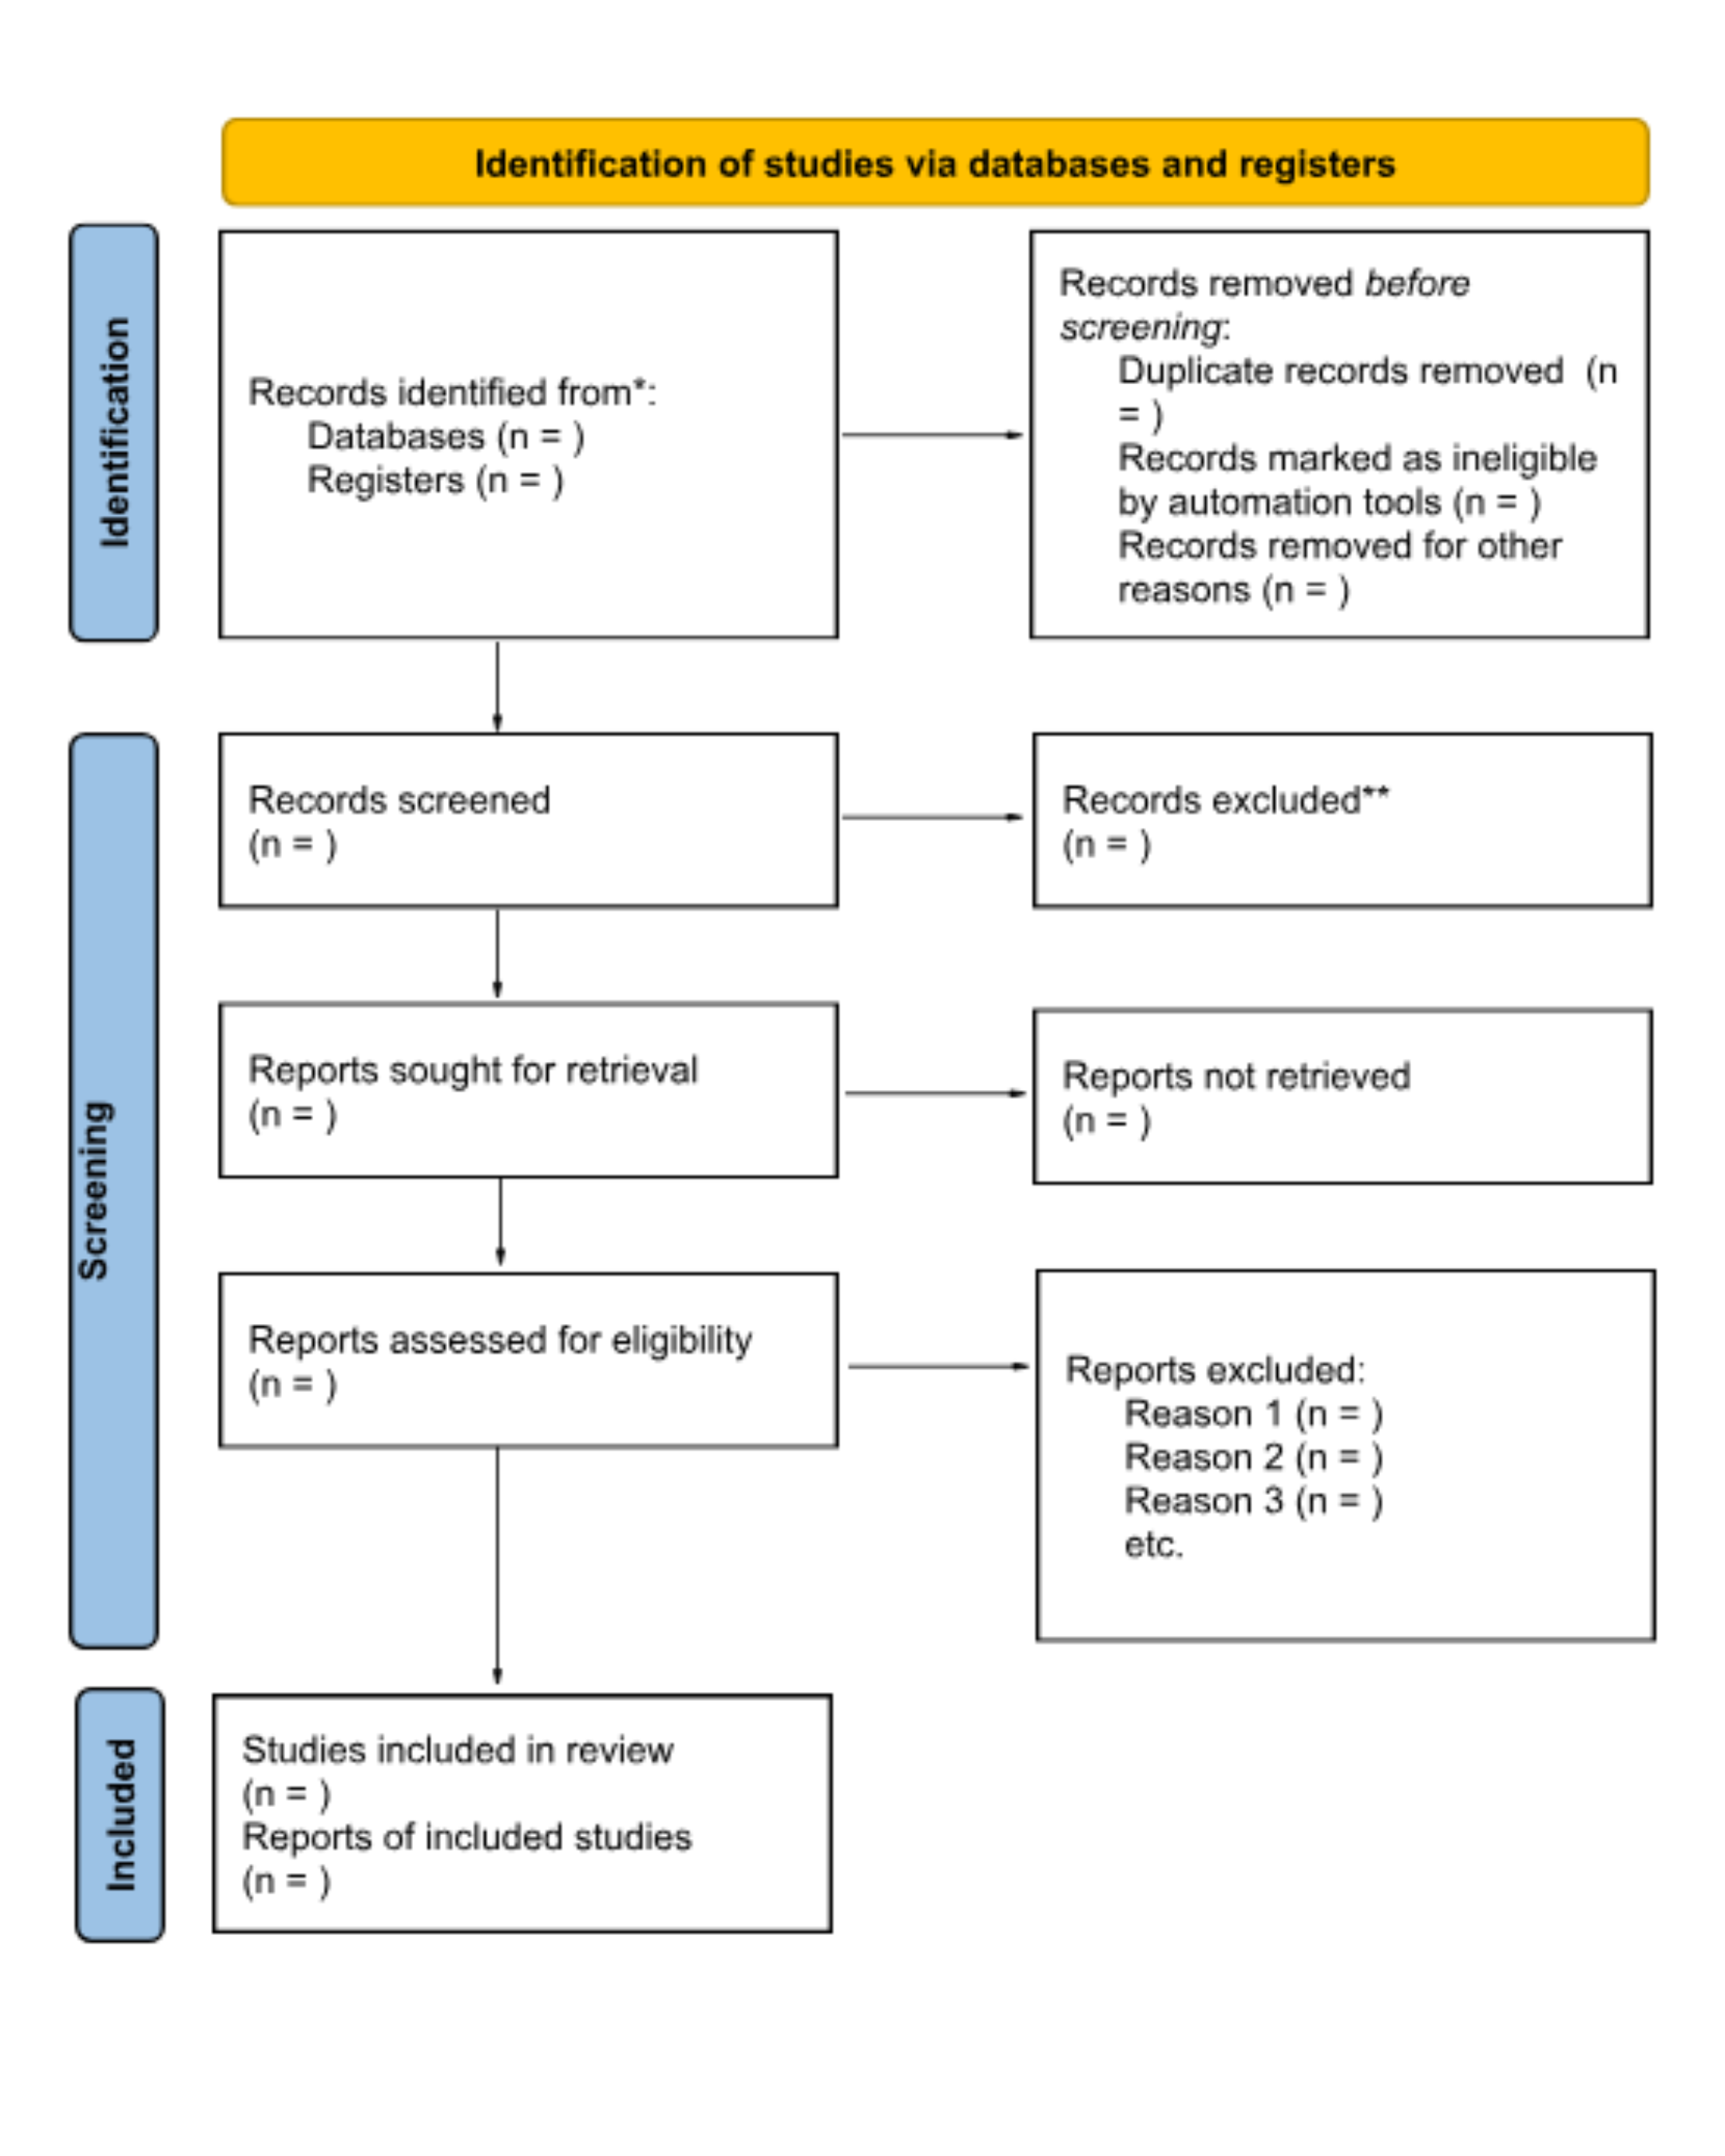
\includegraphics[width=0.9\textwidth]{figuras/prisma-fluxograma.png}
\fonte{\citeonline{prisma_2020}}
\end{figure}

São reconhecidas, ainda, cinco ameaças à validade do mapeamento. A primeira é a cobertura incompleta inerente ao conjunto de bases escolhidas, mitigada parcialmente pela amplitude do agregador empregado na execução inicial. A segunda decorre dos vieses de seleção e extração, mitigada pela documentação completa dos critérios e pela validação contra o conjunto-semente nomeado. A terceira reside em eventual subinclusividade ou superinclusividade das \emph{strings} de busca, mitigada pelas rodadas de calibração registradas na memória técnica do trabalho. A quarta é a datação dos resultados, registrada explicitamente em cada execução de busca. A quinta é a cobertura de literatura cinza, restrita conforme o critério CE6.

\section{Especificação formal e validação experimental}
\label{sec-frente-experimental}

A linha experimental reúne duas atividades acopladas. A primeira especifica formalmente o núcleo do protocolo de estado de sessão como um sistema de transições, com canal de replicação assíncrona abstrato, e verifica os invariantes declarados por \emph{model checking}. A segunda implementa e valida experimentalmente os mesmos invariantes em um \emph{cluster} Infinispan, com injeção parametrizada de falhas e instrumentação do programa de carga para detectar violações e medir percentis de latência. O recorte aplicado a ambas as atividades é derivado dos achados da linha de mapeamento. No escopo correspondente ao Trabalho de Conclusão de Curso~I, esta linha cobre a preparação do ambiente, a implementação do programa de carga, a especificação formal inicial do modelo (ainda sem falhas explicitamente modeladas) e a execução de \emph{baseline} experimental parcial sob um subconjunto dos cenários de falha previstos.  Os resultados parciais são reportados no Capítulo~\ref{cap-desenvolvimento}.

\section*{Escolha do ferramental de verificação}
\label{sec-escolha-ferramenta}

A verificação formal do núcleo do protocolo admite ferramentas de naturezas distintas, e a seleção pondera expressividade, custo de prova e ajuste ao recorte do trabalho. A análise relacional limitada por escopo com Alloy \citep{jackson_software_abstractions_2012} verifica invariantes estruturais sobre relações, mas opera sob limite de escopo e perde força na representação de um canal assíncrono com muitos passos de execução. O \emph{model checking} explícito de protocolos com SPIN e a linguagem Promela \citep{holzmann_spin_2004} é maduro para sistemas de processos comunicantes, porém opera em nível mais baixo e oferece menos expressividade para invariantes em teoria de conjuntos sobre os mapas que descrevem o estado de sessão. Os assistentes de prova como Coq e Isabelle provam propriedades sem limite de estados, mas exigem prova manual interativa, esforço desproporcional ao recorte do protocolo e ao cronograma das duas etapas. As abordagens empíricas para a mesma garantia, como testes baseados em propriedades, engenharia do caos e verificação a posteriori do tipo Jepsen \citep{bailis_kingsbury_network_2014}, validam o que o sistema executa, mas não certificam o que é possível no espaço de estados, e no presente trabalho já estão refletidas na vertente experimental descrita nesta seção.

A escolha recai sobre o conjunto TLA+ e TLC por quatro razões. A semântica de especificação de \citet{lamport_specifying_systems_2002} mapeia de forma direta os invariantes de segurança como propriedades de invariância, expressas pelo operador temporal $\square P$, que afirma que $P$ vale em todo estado da execução, e as propriedades de convergência sob quiescência declaradas na Seção~\ref{sec-invariantes}. O canal de replicação assíncrona é modelado como multiconjunto de mensagens com entrega não determinística, o que reproduz reordenação e atraso sem premissas de sincronia.  Há maturidade da linguagem e registro de aplicação industrial em sistemas de replicação \citep{newcombe_aws_formal_methods_2015, newcombe_aws_tla_2014}, o que reduz risco metodológico. Por fim, a cardinalidade reduzida do recorte (poucas identidades, sessões e réplicas, conforme o parâmetro T21 da Seção~\ref{sec-parametros}) mantém a verificação exaustiva do TLC tratável.  Dentro do mesmo ecossistema TLA+, o tradutor Apalache para verificação simbólica e o detector Must \citep{enea_must_2024} para protocolos assíncronos com falhas figuram como caminhos de escalabilidade reservados à etapa subsequente, quando o espaço de estados crescer com a inclusão explícita de falhas. 

\section*{Operações modeladas}
\label{sec-operacoes}

O protocolo de estado de sessão compreende sete operações sobre um par de mapas globais: o mapa $\sigma : \mathcal{S} \to \{\textsf{Valid}, \textsf{Invalid}(\textsf{reason})\}$, que associa a cada sessão $s$ seu estado lógico, e o mapa $\beta : \mathcal{U} \to \mathbb{N} \times \{\textsf{Free}, \textsf{Blocked}\}$, que associa a cada identidade $u$ o contador de tentativas e a marca de bloqueio.  As operações ficam definidas a seguir, com precondições e efeitos.

\textbf{O1, \emph{login}.} Cria nova sessão $s$ para uma identidade $u$ após validação de credenciais. Precondição: $\beta(u).\textsf{marca} = \textsf{Free}$. Efeito: $\sigma' = \sigma \cup \{s \mapsto \textsf{Valid}\}$, $\beta'(u).\textsf{counter} = 0$ (reposição implícita por sucesso). Caso a precondição falhe, a operação retorna o código de erro $\textsf{IdentityBlocked}$ sem alterar o estado. 

\textbf{O2, validação.} Operação de leitura que consulta o estado lógico atual de uma sessão. Sem efeitos sobre $\sigma$ ou $\beta$; retorna $\sigma(s)$ se $s \in \textsf{dom}(\sigma)$ e $\textsf{NotFound}$ caso contrário.

\textbf{O3, \emph{logout}.} Marca a sessão $s$ como inválida com motivo registrado. Efeito: $\sigma' = \sigma[s \mapsto \textsf{Invalid}(\textsf{logout})]$. A operação é idempotente: aplicar O3 duas vezes sobre a mesma sessão produz o mesmo estado.

\textbf{O4, incremento de tentativas falhas.} Adiciona uma unidade ao contador da identidade $u$ após autenticação falha. Efeito: $\beta'(u).\textsf{counter} = \beta(u).\textsf{counter} + 1$; se $\beta'(u).\textsf{counter} \ge \theta$, em que $\theta$ é o limiar de bloqueio (parâmetro do sistema), então $\beta'(u).\textsf{marca} = \textsf{Blocked}$ e $\sigma' = \sigma[s \mapsto \textsf{Invalid}(\textsf{blocked})]$ para toda sessão $s$ de $u$. 

\textbf{O5, reposição de tentativas.} Zera o contador da identidade $u$ após sucesso de \emph{login} dentro da janela. Efeito: $\beta'(u).\textsf{counter} = 0$, sem alterar a marca de bloqueio.

\textbf{O6, bloqueio administrativo.} Marca a identidade $u$ como bloqueada e invalida toda sessão ativa associada, independentemente do contador. Efeito: $\beta'(u).\textsf{marca} = \textsf{Blocked}$ e $\sigma' = \sigma[s \mapsto \textsf{Invalid}(\textsf{admin\_block})]$ para toda sessão $s$ de $u$.

\textbf{O7, desbloqueio.} Remove a marca de bloqueio e zera o contador. Efeito: $\beta'(u).\textsf{marca} = \textsf{Free}$, $\beta'(u).\textsf{counter} = 0$. Não recria sessões previamente invalidadas.

\revini{MET-13}Cada operação registra marcas de tempo de início e fim com precisão de nanossegundos, o servidor de conexão do cliente, o código de retorno e a chave, e alimenta as métricas de latência e a detecção de violações descritas na Seção~\ref{sec-metricas}.\revfim{MET-13}

\section*{Modelo de falhas}
\label{sec-falhas}

Quatro classes de falha são consideradas no escopo do Trabalho de Conclusão de Curso~I, cada uma parametrizada para reprodução experimental controlada. \revini{MET-14}As classes se enquadram na taxonomia de \citet{avizienis_taxonomy_2004}.\revfim{MET-14}

\textbf{F1, \emph{crash} silencioso de nó.} Um nó deixa de responder sem aviso prévio. Parâmetros: identificador do nó alvo, instante de início $t_\textsf{crash}$ medido em segundos desde o início da execução, e duração da indisponibilidade $\Delta_\textsf{crash}$ (com $\Delta_\textsf{crash} = \infty$ correspondendo a falha permanente). A reativação do nó, quando ocorre, expõe o cenário de recuperação (\emph{crash-recovery}) e ativa o procedimento de \emph{state transfer}. \revini{MET-15}A pilha de comunicação do \emph{cluster} tem dois detectores de falha: o FD\_ALL3, que suspeita de um nó depois de um intervalo sem mensagens de presença (T16), e o FD\_SOCK2, que suspeita assim que a conexão TCP com o nó se fecha. Para que a queda seja silenciosa e detectada pelo FD\_ALL3, a interface de rede do nó é desativada antes que o processo seja encerrado (Seção~\ref{sec-protocolo-rebaseline}).\revfim{MET-15}

\textbf{F2, partição de rede entre subconjuntos do \emph{cluster}.} O conjunto de nós é dividido em dois ou mais subconjuntos $\{P_1, P_2, \ldots\}$ tais que a comunicação entre subconjuntos distintos é descartada por um intervalo $[t_\textsf{part}, t_\textsf{part} + \Delta_\textsf{part}]$. Dentro de cada subconjunto, a comunicação permanece normal. Esta classe fica reservada para o Trabalho de Conclusão de Curso~II (Decisão 011, ponto 11), com F1 e F3 cobrindo o escopo experimental do Trabalho de Conclusão de Curso~I. \revini{MET-16}No experimento, um nó é isolado dos outros dois (minoria de um nó), e o fim do intervalo dispara a fusão das partições.\revfim{MET-16}

\textbf{F3, introdução de atraso e \emph{jitter} no canal.} O atraso aplicado a cada mensagem é amostrado de uma distribuição com média $\mu$ e desvio padrão $\sigma$ (parâmetros do cenário), com aplicação via \texttt{tc-netem} \citep{netem_manpage} no \emph{network namespace} de cada \emph{container}. A distribuição padrão adotada é lognormal, escolhida por aproximar a cauda longa observada empiricamente em redes reais; alternativas exponencial e uniforme ficam configuráveis para análise de sensibilidade. 

\textbf{F4, mudança de topologia que induz \emph{state transfer}.} A adição ou remoção controlada de um nó durante carga ativa o rebalanceamento do Infinispan e dispara transferência de segmentos entre nós, com janela de inconsistência transitória durante a propagação. Parâmetros: tipo de evento (entrada ou saída de nó), nó alvo, instante. F4 fica como ampliação opcional no Trabalho de Conclusão de Curso~I, com execução completa no Trabalho de Conclusão de Curso~II. 

Falhas bizantinas (mensagens corrompidas ou maliciosas) estão fora de escopo, \revini{MET-57}dado que o modelo de falhas deste trabalho supõe canal honesto\revfim{MET-57} (CE6 do protocolo do mapeamento, Seção~\ref{sec-ms}). Cenários multi-site (\emph{cross-site} replication) ficam reservados para a etapa subsequente do trabalho. 

\section*{Invariantes alvo}
\label{sec-invariantes}

O conjunto inicial de invariantes verificados no Trabalho de Conclusão de Curso~I tem seis elementos, declarados sobre os mapas $\sigma$ e $\beta$ definidos na Seção~\ref{sec-operacoes}, sobre o conjunto de réplicas $\mathcal{R}$, e sobre a sequência temporal de estados globais $\{S_t\}_{t \ge 0}$. Os quatro primeiros são propriedades de segurança e devem valer em todo estado alcançável. Os dois últimos são propriedades de convergência, próprias da consistência eventual, e valem sob hipótese de quiescência, ou seja, no estado em que não há operações em andamento e, cessadas as operações, as réplicas convergem para o mesmo valor. 

\textbf{I1, irreversibilidade da invalidação por \emph{logout}.} A partir do momento em que uma sessão atinge o estado inválido com motivo \emph{logout}, nenhum estado futuro pode ter essa mesma sessão como válida:
\[
\forall s \in \mathcal{S}, \forall t \ge 0: \quad \sigma_t(s) = \textsf{Invalid}(\textsf{logout}) \Rightarrow \forall t' \ge t: \, \sigma_{t'}(s) \ne \textsf{Valid}.
\]

\textbf{I2, consistência de bloqueio.} Enquanto uma identidade estiver marcada como bloqueada, nenhuma sessão associada pode ser validada como ativa:
\[
\forall u \in \mathcal{U}, \forall t: \quad \beta_t(u).\textsf{marca} = \textsf{Blocked} \Rightarrow \forall s \in \textsf{sessions}(u): \, \sigma_t(s) \ne \textsf{Valid}.
\]


\textbf{I3, monotonicidade local do contador.} Em cada réplica $r \in \mathcal{R}$, na ausência de reposição (O5) e desbloqueio (O7) entre dois instantes $t_1 < t_2$, o contador é não-decrescente:
\[
\forall u, \forall r, \forall t_1 < t_2: \quad \beta_{r, t_1}(u).\textsf{counter} \le \beta_{r, t_2}(u).\textsf{counter},
\]
restrito ao intervalo em que nenhuma operação O5 ou O7 sobre $u$ é aplicada em $r$.

\textbf{I4, unicidade do motivo de invalidação.} Uma vez fixado o motivo de invalidação de uma sessão, ele não é reescrito por outra causa:
\[
\forall s, \forall t: \quad \sigma_t(s) = \textsf{Invalid}(m) \, \land \, m \ne \bot \Rightarrow \forall t' > t: \, \sigma_{t'}(s) = \textsf{Invalid}(m).
\]

\textbf{I5, convergência do estado lógico (sob quiescência).} Após o cessar das operações e a entrega de todas as mensagens pendentes pelos canais (estado de quiescência $Q$), todas as réplicas observam o mesmo estado lógico para cada sessão:
\[
\textsf{quiescent}(Q) \Rightarrow \forall s, \forall r_1, r_2 \in \mathcal{R}: \, \sigma_{r_1}(s) = \sigma_{r_2}(s).
\]


\textbf{I6, convergência do contador (sob quiescência).} Sob a mesma hipótese, o contador converge entre réplicas:
\[
\textsf{quiescent}(Q) \Rightarrow \forall u, \forall r_1, r_2 \in \mathcal{R}: \, \beta_{r_1}(u).\textsf{counter} = \beta_{r_2}(u).\textsf{counter}.
\]


Os invariantes I3, I5 e I6 reconhecem explicitamente a separação entre estado local de cada réplica e estado lógico global; I5 e I6 derivam diretamente da Consistência Eventual Forte de \citet{shapiro_crdt_2011} aplicada aos tipos de dados subjacentes (registrador para $\sigma$, contador para $\beta.\textsf{counter}$). 

\section*{Métricas e critérios}
\label{sec-metricas}

A avaliação adota cinco métricas primárias coletadas por execução de cenário.

\textbf{Latência por operação.} Coletada como distribuição empírica, com cálculo de percentis p50, p95, p99 e p99,9 conforme prática consolidada para sistemas com cauda longa \citep{dean_barroso_tail_2013, google_sre_slo}. A coleta usa marcas de tempo de início e fim com precisão de nanossegundos, registradas pelo programa de carga, com agregação em janelas configuráveis para análise temporal.

\textbf{Taxa de violação por invariante.} Contabilizada como número de eventos detectados por unidade de tempo e por operação. A detecção segue dois caminhos (Seção~\ref{sec-arquitetura}): verificação imediata após cada operação para violações observáveis localmente (I1 a I4), e auditoria periódica em janelas de quiescência para violações de convergência (I5 e I6). Cada violação registrada inclui o invariante atingido, o estado relevante das réplicas e o histórico de operações que o produziu. 

\textbf{Tempo de recuperação.} Mede o intervalo $\Delta_\textsf{rec} = t_\textsf{base} - t_\textsf{fim-falha}$ entre o fim da injeção de uma falha (instante $t_\textsf{fim-falha}$) e o retorno da taxa de erro à linha de base (instante $t_\textsf{base}$, definido como o primeiro instante em que a taxa de erro permanece dentro de uma margem $\epsilon$ da pré-falha por uma janela de $W$ segundos).

\textbf{Tempo de convergência.} Mede o intervalo $\Delta_\textsf{conv}$ entre o fim da falha e o desaparecimento de divergências entre réplicas (detectado pela auditoria periódica reportando $\sigma_{r_1} = \sigma_{r_2}$ e $\beta_{r_1} = \beta_{r_2}$ para todo par $(r_1, r_2)$ de réplicas). 

\textbf{Taxa de erro.} Contabiliza as requisições que retornam código distinto de sucesso, sem implicar necessariamente violação de invariante. Inclui erros transitórios de comunicação, recusa por bloqueio, \emph{timeouts} e códigos específicos do cliente Hot Rod.

Métricas secundárias, coletadas via API e logs do Infinispan, incluem uso de CPU por nó, memória do \emph{heap}, número de eventos de rebalanceamento, número de mensagens RPC trocadas e tamanho da fila de propagação assíncrona \citep{infinispan_metrics}. A exposição segue o formato OpenMetrics \citep{openmetrics_spec}, com integração via JMX \citep{jmx_oracle}, e admite coleta por agente Prometheus opcional \citep{prometheus_docs}. 

Os critérios de comparação entre o \emph{baseline} estático e a configuração com o controlador heurístico, planejados para o Trabalho de Conclusão de Curso~II, exigem três condições simultâneas. \revini{MET-28}A primeira é redução estatisticamente significativa da taxa de violação, avaliada pelo teste não paramétrico de Mann-Whitney sobre as amostras de cada cenário ($\alpha = 0{,}05$).\revfim{MET-28} A segunda é manutenção das latências p95 e p99 dentro de margem aceitável, definida como degradação máxima de 10\% em relação ao \emph{baseline}, com intervalo de confiança de 95\%. A terceira é a auditabilidade das decisões do controlador: cada ação aplicada deve ser rastreável até a regra que a motivou, com registro do gatilho (observável + limiar), do estado anterior e do estado seguinte do controlador. Os três critérios devem ser cumpridos conjuntamente para que a configuração com controlador seja considerada melhoria sobre o \emph{baseline}. 

\section*{Parâmetros experimentais e fundamentação na literatura}
\label{sec-parametros}

A definição dos parâmetros operacionais do \emph{baseline} segue três princípios. O primeiro é a compatibilidade com a literatura de avaliação de \emph{key-value stores} e \emph{data grids} sob carga com cauda longa, exemplificada por \citet{jaiman_tailx_2020} no caso de Cassandra com YCSB e por \citet{decandia_dynamo_2007} no caso de Dynamo. O segundo é a aderência à configuração recomendada na documentação oficial do Infinispan \revini{MET-58}(\citeauthor{infinispan_docs_stable}, \citeyear{infinispan_docs_stable}, \citeyear{infinispan_metrics}, \citeyear{infinispan_tuning})\revfim{MET-58}, de modo que o experimento meça o comportamento do sistema em configuração próxima da praticada em produção. O terceiro é a proporcionalidade ao escopo do Trabalho de Conclusão de Curso~I (Decisão de recorte registrada na Seção~\ref{sec-frente-experimental}), que delimita o tamanho do \emph{cluster}, o conjunto de cenários de falha e o volume de operações para que o tempo de execução em \emph{Sem}~9 e 10 fique dentro da janela disponível.

{\scriptsize
\setlength{\tabcolsep}{2pt}
\begin{longtable}{p{0.6cm} p{3.0cm} p{3.5cm} p{2.0cm} p{2.2cm} p{2.7cm}}
\captionsetup{font=normalsize}
\caption{Parâmetros do \emph{baseline} experimental: faixa observada, fonte e valor adotado}
\label{tab-parametros-baseline}\\
\hline
\textbf{ID} & \textbf{Parâmetro} & \textbf{Faixa observada} & \textbf{Fonte} & \textbf{Valor adotado} & \textbf{Justificativa do recorte} \\
\hline
\endfirsthead
\multicolumn{6}{c}{\normalsize \tablename\ \thetable\ -- continuação} \\
\hline
\textbf{ID} & \textbf{Parâmetro} & \textbf{Faixa observada} & \textbf{Fonte} & \textbf{Valor adotado} & \textbf{Justificativa do recorte} \\
\hline
\endhead
\hline
\multicolumn{6}{r}{\footnotesize \emph{continua na próxima página}} \\
\endfoot
\hline
\endlastfoot
T1 & Modo de replicação & DIST\_SYNC, DIST\_ASYNC, REPL\_SYNC, REPL\_ASYNC & \citealt{infinispan_docs_stable} & DIST\_ASYNC (alvo) e DIST\_SYNC (controle) & objeto de estudo é replicação assíncrona \\
T2 & Número de nós & 3 mínimo; 16 em estudos comparáveis & \revini{MET-30}\citealt{jaiman_tailx_2020, yuan_simple_testing_2014} & 3 & escopo TCC-I; tolerância mínima a 1 falha; falhas de produção reproduzíveis com até 3 nós\revfim{MET-30} \\
T3 & \texttt{numOwners} & 2 (padrão); $>2$ aumenta durabilidade & \citealt{infinispan_tuning} & 2 & padrão da documentação \\
T4 & \texttt{numSegments} & 256 (padrão); $20 \times N$ para $N>20$ & \citealt{infinispan_tuning} & 256 & dentro da faixa padrão para $N=3$ \\
T5 & Tamanho do \emph{payload} & 1 KB típico de sessão; 1 KB--2 MB em estudos de cauda & \citealt{jaiman_tailx_2020} & 1 KB fixo & representativo de objeto de sessão \\
T6 & Distribuição de chaves & \revini{MET-50}Zipfian $\rho=0{,}99$ (YCSB); uniforme; \emph{latest}\revfim{MET-50} & \citealt{cooper_ycsb_2010, jaiman_tailx_2020} & Zipfian $\rho=0{,}99$ & expõe a cauda; comparável com a literatura \\
T7 & Mistura de operações & 50/50, 95/5, 100R, leitura-modifica-escrita & \citealt{cooper_ycsb_2010, jaiman_tailx_2020} & 50/50 (cenário S1) + 95/5 (cenário S2) & 50/50 modela \emph{session store} de escrita ativa; 95/5 isola comportamento de validação \\
T8 & Cardinalidade de chaves & 50\,000 em \emph{benchmarks} sintéticos; 20\,M em estudos de cauda & \citealt{jaiman_tailx_2020} & 100\,000 & forma cauda Zipfian; cabe em \emph{heap} de poucos GB por nó \\
T9 & Operações por execução & \revini{MET-51}$10^6$--$10^7$\revfim{MET-51} & \citealt{jaiman_tailx_2020} & $10^6$ & viabiliza p99,9 estável ($n=1\,000$ amostras na cauda) \\
T10 & Repetições por cenário & 5 em estudos comparáveis & \citealt{jaiman_tailx_2020} & 30 & conservador para testes não paramétricos \\
T11 & \emph{Warm-up} & \revini{MET-52}fases de \emph{load} e \emph{run} separadas em YCSB & \citealt{cooper_ycsb_2010}\revfim{MET-52} & 60\,s ou 10\,\% do total; descarte das primeiras 5\,\% das amostras & estabilização de JIT, alocadores e cache \\
T12 & Carga (alvo) & 75\,\% do pico medido & \citealt{jaiman_tailx_2020} & 75\,\% do pico do piloto sem falhas & evita saturação; expõe variabilidade \\
T13 & Percentis reportados & p95 e p99 (mínimo da indústria); p99,9 em \emph{key-value stores} & \citealt{dean_barroso_tail_2013, decandia_dynamo_2007, google_sre_slo} & p50, p95, p99 obrigatórios; p99,9 quando $n \ge 10^6$ & padrão da literatura; p99,9 é estatisticamente
fiável com o volume adotado \\
T14 & Duração por cenário & \revini{MET-53}não reportada (estudos fixam número de operações)\revfim{MET-53} & \citealt{jaiman_tailx_2020} & 10\,min sem falha; 30\,min com falha & inclui a janela de detecção (T16) e estabilização \\
T15 & MTU & 1500 (padrão); até 9000 (\emph{jumbo}) & \citealt{infinispan_tuning} & 1500 & infraestrutura em \emph{containers} sem \emph{jumbo} controlado \\
T16 & Detecção de falha (FD\_ALL3) & \revini{MET-54}\emph{heartbeat} 8000\,ms, \emph{timeout} 40000\,ms, padrão da pilha JGroups do servidor (conferido na configuração do \emph{cluster}) & O autor\revfim{MET-54} & padrões mantidos & reproduz produção; define duração mínima de F1 \\
T17 & Falha F1 (\emph{crash}) & nó silencioso; reentrada com \emph{state transfer} & \citealt{infinispan_docs_stable} & 1 nó; $\Delta_\text{crash}=60$\,s; reentrada ativa & \revini{MET-31}maior que o \emph{timeout} de T16; ativa convergência (I5, I6)\revfim{MET-31} \\
T18 & Falha F3 (atraso/\emph{jitter}) & \revini{MET-33}atraso com média, desvio e distribuição configuráveis & \citealt{netem_manpage} & \revini{MET-32}$+50$\,ms no p99 via \texttt{tc-netem}\revfim{MET-32} & valor de engenharia, sem fonte empírica; calibrável\revfim{MET-33} \\
T19 & Métricas coletadas & latência, vazão, \emph{hit ratio}, RPC, \emph{state transfer} & \citealt{infinispan_metrics} & M1--M7 (Seção~\ref{sec-metricas}) & mapeamento 1:1 com os medidores expostos \\
T20 & Endpoint de métricas & JMX; OpenMetrics & \citealt{infinispan_metrics} & OpenMetrics; Prometheus opcional & padrão atual da documentação \\
T21 & Espaço de estados (TLC) & \revini{MET-34}cardinalidades pequenas (2--3 por \emph{sort}) em verificações industriais; falhas de produção com até 3 nós & \citealt{yu_lamport_tla_modelchecking_1999, newcombe_aws_tla_2014, yuan_simple_testing_2014}\revfim{MET-34} & 2--3 identidades, sessões e réplicas & expõe entrelaçamento concorrente; \emph{model checking}
incremental \\
T22 & Análise estatística & Mann-Whitney/Wilcoxon; \emph{bootstrap} para IC de percentis & \revini{MET-35}\citealt{mann_whitney_1947, efron_tibshirani_bootstrap_1993}\revfim{MET-35} & Mann-Whitney por percentil; \emph{bootstrap} com 10\,000 reamostragens para IC 95\,\% & distribuições assimétricas de latência \\
\end{longtable}
}
\fonte{O autor, com base em \citet{cooper_ycsb_2010}, \citet{decandia_dynamo_2007}, \citet{dean_barroso_tail_2013}, \citet{google_sre_slo}, \citet{infinispan_docs_stable}, \citet{infinispan_metrics}, \citet{infinispan_tuning}, \citet{jaiman_tailx_2020},
\revini{MET-49}\revfim{MET-49}\citet{yu_lamport_tla_modelchecking_1999}\revini{MET-36}, \citet{newcombe_aws_tla_2014}, \citet{yuan_simple_testing_2014}, \citet{netem_manpage}, \citet{mann_whitney_1947} e \citet{efron_tibshirani_bootstrap_1993}.\revfim{MET-36}}

 A Tabela~\ref{tab-parametros-baseline} sintetiza a análise, com a faixa observada na literatura ou na documentação oficial, a fonte principal e o valor adotado, e a justificativa do recorte. A tabela explicita três escolhas que merecem comentário. A combinação $10^6$ operações por execução (T9) com 30 repetições por cenário (T10) decorre da necessidade de estimar p99 e, quando aplicável, p99,9 sob incerteza controlada: com $10^6$ amostras, o p99,9 dispõe de $10^3$ observações na cauda, \revini{MET-37}base para um intervalo de confiança \emph{bootstrap} \citep{efron_tibshirani_bootstrap_1993}. Com 30 repetições, comparações entre cenários por percentil podem ser feitas pelo teste de \citet{mann_whitney_1947}, sem hipótese de normalidade,\revfim{MET-37} condição necessária dada a assimetria das distribuições de latência observadas em sistemas com cauda longa. A escolha de Zipfian $\rho=0{,}99$ (T6) e mistura 50/50 (T7) reproduz o setup de \citet{jaiman_tailx_2020} e a definição de \emph{Workload~A} do YCSB, descrito por \citet{cooper_ycsb_2010} como ``\emph{session store recording recent actions}'', e portanto põe o experimento em registro comparável com o estudo de cauda em Cassandra. A escolha dos valores padrão de detecção de falha (T16) deixa o cenário F1 (T17) com duração mínima alinhada ao \emph{timeout} de 40\,s, condição necessária para que o evento de falha seja registrado pelo \emph{cluster} antes do encerramento da janela experimental. 

\section*{Carga sintética dos cenários S1 e S2}
\label{sec-carga}

\revini{MET-39}Os cenários S1 e S2 da linha T7 da Tabela~\ref{tab-parametros-baseline} sorteiam, a cada iteração de cada \emph{thread} do programa de carga, uma operação com pesos fixos. Em S1, os pesos são 50\,\% de validação (O2), 25\,\% de \emph{login} (O1), 10\,\% de \emph{logout} (O3), 10\,\% de incremento de tentativas falhas (O4) e 5\,\% de reposição de tentativas (O5). Em S2, os pesos na mesma ordem são 95\,\%, 3\,\%, 1\,\%, 1\,\% e 0\,\%. O \emph{login} abre uma tríade: quando ele é aceito, a mesma \emph{thread} valida e encerra a sessão recém-criada, e os três eventos entram no registro. As validações e os \emph{logouts} sorteados fora da tríade, chamados aqui de isolados, recaem sobre chaves de sessão escolhidas pela distribuição Zipfian de T6, no universo de chaves de T8.

Antes do aquecimento de cada execução, o programa esvazia os dois \emph{caches} do modo de replicação em uso, confere que ambos ficaram vazios e encerra a execução com código de erro próprio se isso não ocorrer. Cada \emph{thread} $t$ usa, no \emph{login}, oito identidades próprias, \texttt{user-}$t$\texttt{-}$k$ com $k = 0, \dots, 7$, tomadas em rodízio, que nunca recebem O4 nem O5. As operações O4 e O5 atuam sobre uma identidade separada por \emph{thread}, \texttt{lim-}$t$, de modo que o bloqueio por limite continua exercitado sem atingir as identidades de \emph{login}. As chaves lidas pelas operações isoladas existem no \emph{cache}, conforme o esquema de gerações descrito a seguir. O rodízio não consome os geradores da mistura nem o de chaves.

A versão da mistura adotada nas medições organiza as chaves de sessão em \emph{slots}. O sorteio Zipfian define o \emph{slot} $k$, e um vetor compartilhado entre as \emph{threads} guarda a geração corrente $g_k$ de cada \emph{slot}. Antes do aquecimento, uma fase de carga grava, para cada um dos $10^5$ \emph{slots}, a geração 0 como sessão já invalidada por \emph{logout} e a geração 1 como sessão válida, o que soma $2 \times 10^5$ entradas e fixa $g_k = 1$. A sessão do \emph{slot} $k$ pertence à identidade \texttt{user-}$((k-1) \bmod T)$\texttt{-}$(\lfloor (k-1)/T \rfloor \bmod 8)$, em que $T$ é o número de \emph{threads}, a mesma em todas as gerações do \emph{slot}. A validação isolada lê a geração corrente, exceto quando um sorteio de Bernoulli independente, com probabilidade $p = 0{,}05$, a desvia para a geração anterior. Esse desvio representa um cliente que ainda apresenta um \emph{token} antigo. O valor de $p$ é uma premissa de engenharia, declarada como tal, e não a medida de um serviço real. O \emph{logout} isolado toma uma trava da faixa do \emph{slot} ($k \bmod 1024$), invalida a geração corrente, que é a operação medida e registrada, grava como válida a geração $g_k + 1$ e só então avança $g_k$. Essa gravação de reposição não emite evento, não entra na latência medida e não passa pelo auditor. Se o \emph{logout} retornar erro, não há reposição nem avanço. Se a reposição falhar, a geração não avança, e as validações seguem sobre a sessão já invalidada até o próximo \emph{logout} do \emph{slot}.

O desenho tem três consequências declaradas. A fração de respostas \textsf{Invalid} entre as validações isoladas fica estacionária desde o primeiro evento, próxima de $p$ acrescida da corrida entre uma validação e um \emph{logout} do mesmo \emph{slot}. A reposição acrescenta ao \emph{cluster} uma escrita por \emph{logout} isolado, ausente do registro de eventos, em número próximo de 10\,\% das operações em S1 e de 1\,\% em S2. A trava serializa no cliente os \emph{logouts} isolados de uma mesma faixa de \emph{slot}, que portanto não concorrem entre si, e a espera pela trava fica fora da latência medida. Os critérios de estacionariedade foram fixados antes de qualquer execução dessa versão da mistura. A fração \textsf{Invalid} entre as validações isoladas pode diferir no máximo 1,0 ponto percentual entre o primeiro e o terceiro terço da janela de medição (critério C1) e deve ficar no intervalo $[4{,}5\,\%;\ 6{,}5\,\%]$ (C2). Com $n$ validações isoladas e $k$ leituras de \emph{token} antigo, a execução deve satisfazer $|k/n - 0{,}05| \le 3{,}2905 \sqrt{0{,}05 \cdot 0{,}95 / n}$ (C3), região de aceitação do teste de $H_0\colon p = 0{,}05$ ao nível de 0,1\,\% pela aproximação normal da binomial, aplicada somente quando $n \cdot 0{,}05 \cdot 0{,}95 \ge 100$, limite adotado por cautela diante da cobertura errática dessa aproximação \citep{brown_cai_dasgupta_binomial_2001}. As contagens de C3 lidas na saída do programa e no registro de eventos podem diferir em até quatro eventos, o número de \emph{threads}, por causa da fronteira da janela de medição. Execução fora dessas tolerâncias é recusada.

O \emph{logout} e a cascata de invalidação do bloqueio administrativo (O6) invalidam sessões por escrita condicional à versão lida. O programa lê a sessão com sua versão e a substitui pela versão invalidada somente se a versão não tiver mudado; em caso de conflito, relê a sessão e tenta de novo, até três tentativas. A primeira invalidação vence, e o motivo registrado não muda depois. Uma invalidação que perde a escrita condicional e relê a sessão já invalidada é contada como invalidação perdida e não altera o estado. Se a sessão continuar válida, com versão alterada, depois da terceira tentativa, a operação termina com o código \texttt{ERROR\_TRANSPORT}, e um contador próprio de conflitos esgotados separa esse caso dos erros de transporte na análise. Os \emph{caches} permanecem não transacionais. O servidor emite uma vez por processo o aviso \texttt{ISPN006010}, segundo o qual operações condicionais devem ser usadas com \emph{caches} transacionais porque, de outro modo, ``\emph{data inconsistency issues could arise under failure situations}''. O guia do cliente Hot Rod faz a mesma recomendação, para que no \emph{failover} as operações condicionais não fiquem parcialmente aplicadas, com entradas conflitantes em nós diferentes \citep{infinispan_hotrod_java_15}, e o guia de configuração adverte que a divisão do \emph{cluster} em partições pode causar perda ou inconsistência de dados qualquer que seja a estratégia de tratamento ou a política de \emph{merge} \citep{infinispan_configuring_15}. A configuração não transacional foi mantida porque a adoção de \emph{caches} transacionais mudaria o sistema medido. Por isso, uma violação de I4 ou uma invalidação perdida observada sob falha (queda de nó, partição ou fusão de partições) é tratada na análise como efeito do \emph{grid}, e não da aplicação.

O \emph{login} relê a identidade depois de gravar a sessão. Se a releitura encontrar a identidade bloqueada, o próprio \emph{login} invalida a sessão recém-gravada com o motivo de bloqueio administrativo, pelo mesmo caminho condicional da cascata, e retorna recusa por bloqueio. Essa dupla checagem fecha, em \texttt{DIST\_SYNC}, a corrida entre um \emph{login} e um bloqueio concorrente da mesma identidade: o \emph{login} escreve a sessão e lê a identidade, o bloqueio escreve a identidade e lê as sessões, e, com operações linearizáveis, ao menos um dos dois observa a escrita do outro. Em \texttt{DIST\_ASYNC}, a releitura pode encontrar uma réplica atrasada, e o que restar dessa corrida é medida do \emph{grid}. A releitura custa uma leitura a mais por \emph{login} aceito, incluída na latência medida, e vale em todos os cenários, para que o \emph{login} meça a mesma operação em todos eles.

O auditor aplica mais três regras à contagem de violações. Uma validação que lê sessão válida sob identidade bloqueada é classificada pelo instante de início da leitura da sessão, comparado com dois marcos do bloqueio (a confirmação da identidade bloqueada e o fim da cascata de invalidação). A leitura anterior à confirmação conta como concorrente, apenas para diagnóstico; a leitura entre a confirmação e o fim da cascata recebe o rótulo de janela de cascata; a leitura sob cascata interrompida por erro recebe o rótulo de cascata incompleta; e somente a leitura posterior ao fim da cascata é registrada como I2. Dentro de uma mesma operação, cada par formado por invariante e sessão é registrado no máximo uma vez para I1 e I4. Um bloqueio cuja cascata esgota as tentativas termina em \texttt{ERROR\_TRANSPORT} com a cascata parcial, e a contagem de invalidações perdidas inclui apenas a invalidação que perdeu a escrita condicional e releu a sessão invalidada. As tabelas de violação contam I1, I4 e I2 a partir do arquivo de violações de cada execução, e uma I2 só entra como violação quando a análise do rastro do cliente a classifica como real. Os rótulos de janela e de cascata incompleta e os contadores de leituras concorrentes são reportados à parte. A leitura de sessão válida sob identidade bloqueada sem marco de bloqueio deve ser nula em \texttt{DIST\_SYNC}. Em \texttt{DIST\_ASYNC}, uma leitura atrasada da identidade depois do desbloqueio produz esse caso por efeito do \emph{grid}, e a contagem é reportada sem servir de critério.

O registro de eventos distingue, na validação, as respostas \texttt{VALID}, \texttt{INVALID} e \texttt{NOT\_FOUND}, e, no \emph{logout}, a chave ausente (\texttt{NOT\_FOUND}) da invalidação concluída. Ao fim de cada execução, um verificador de sanidade lê esse registro, conta os desfechos por operação na janela de medição e emite veredito sobre a coerência entre os desfechos observados e a mistura declarada. O veredito é desfavorável se não houver \emph{login}, se a fração de \emph{logins} aceitos entre aceitos e recusados por bloqueio ficar abaixo de 0,95, se nenhuma validação retornar \texttt{VALID}, se mais de 5\,\% das validações encontrarem a chave ausente, ou se a fração de alguma operação sorteada se afastar mais de 2,0 pontos percentuais do peso nominal do cenário. Esses limiares são fixados no programa de carga antes do piloto e não são ajustados depois de observados os dados. Como a campanha não registra marcadores de fase, as regras se aplicam a todos os eventos da janela de medição, inclusive aos do intervalo sob falha.

O tipo de cada operação, a chave sorteada e a decisão de ler o \emph{token} antigo vêm de três geradores \texttt{java.util.Random} próprios de cada \emph{thread}, derivados da semente da execução, do índice $t$ da \emph{thread} e da repetição $r$ pela expressão $s = \textit{semente} + t + 1\,000\,003 \cdot r$. O gerador de chaves usa $s$ diretamente. Os outros dois combinam $s$ com um sal próprio por ou exclusivo ($\oplus$) e aplicam a função de mistura de 64 bits do gerador SplitMix \citep{steele_lea_flood_splitmix_2014}, na variante usada por \texttt{java.util.SplittableRandom} ($\textsf{mix64}$), de modo que as três sequências sejam distintas: o gerador da mistura recebe a semente $\textsf{mix64}(s \oplus \textsf{SAL\_MISTURA})$, e o do \emph{token} antigo, $\textsf{mix64}(s \oplus \textsf{SAL\_TOKEN})$. Duas execuções com a mesma semente produzem, em cada \emph{thread}, a mesma sequência de intenções, isto é, os mesmos tipos de operação, \emph{slots}, decisões de \emph{token} antigo e identidades de \emph{login}. A intercalação entre \emph{threads}, as respostas do \emph{grid}, as latências, o número de operações por \emph{thread} e o trecho exato coberto pela janela de medição não são reprodutíveis, porque dependem do tempo. Com mais de uma \emph{thread}, o registro de eventos de duas execuções com a mesma semente não coincide, e a reprodutibilidade vale por \emph{thread}.\revfim{MET-39}

\section*{Cenário S3: simulação do ciclo de vida de sessões}
\label{sec-carga-s3}

\revini{MET-40}Os cenários S1 e S2 sorteiam operações com pesos fixos e não contêm bloqueio administrativo nem afinidade entre cliente e nó, de modo que não exercitam a consistência de bloqueio (I2) nem a escrita feita em um nó isolado por partição. O cenário S3 simula uma aplicação web com os defeitos de uma aplicação real: o programa não repara estado, não reconcilia réplicas e não repete operações indefinidamente, e o experimento registra o que o \emph{data grid} entrega nessas condições. Três servidores de aplicação, cada um ligado a um único nó do \emph{cluster}, atendem usuários virtuais fixados a eles, como sob um balanceador com afinidade; um quarto cliente faz o papel de console administrativo. Cada usuário de um primeiro conjunto de identidades faz \emph{login}, valida a sessão a cada página com tempo de pensar aleatório e, ao fim, encerra a sessão ou a abandona, caso em que a aplicação a considera expirada por inatividade e a sessão permanece válida no \emph{grid}. Depois de um \emph{logout} confirmado, o usuário repete validações da sessão encerrada por alguns segundos, como quem usa o botão de voltar do navegador, o que exercita I1 e I4.

Um ator administrativo bloqueia, em intervalos aleatórios, uma identidade com sessão ativa e a desbloqueia depois de um tempo mínimo, o que exercita I2 com cascata de invalidação. Um segundo conjunto de identidades recebe tentativas falhas até o limite, com reposições ocasionais, e mantém o bloqueio por limite separado do administrativo. O cliente tem tempos-limite curtos e no máximo duas retentativas de aplicação, depois das quais a operação conta como falha percebida pelo usuário. As ações de cada usuário são agregadas em ações S3, com a latência percebida, que inclui as retentativas. Os tempos de pensar, as durações de sessão, os intervalos do administrador e os tamanhos dos conjuntos de identidades são premissas de modelagem, sem fonte empírica, e serão fixados no pré-registro da campanha que usar S3. O cenário S3 é o objeto da campanha com F2 e F4 sob carga e da avaliação do controlador (Seção~\ref{sec-avaliacao-controlador}), enquanto a nova medição de referência usa apenas S1 e S2.\revfim{MET-40}

\section*{Protocolo da nova medição de referência}
\label{sec-protocolo-rebaseline}

\revini{MET-41}A nova medição de referência (\emph{rebaseline}) mede os dois modos de replicação da linha T1 na mesma campanha e com o mesmo \emph{jar}: \texttt{DIST\_SYNC} como controle e \texttt{DIST\_ASYNC} como alvo. O protocolo é pré-registrado \citep{nosek_preregistration_2018} antes de qualquer execução e não admite ajuste depois de observados os dados. Uma mudança gera registro novo, que cita o anterior e explica o motivo. A matriz cruza os cenários S1 e S2, com a carga da Seção~\ref{sec-carga}, os dois modos e três condições (sem falha, F1 e F3), em dez repetições de 300\,s por célula, o que soma 120 execuções, sem o controlador. Cada execução usa quatro \emph{threads} e um \emph{cluster} de três nós com a imagem \texttt{quay.io/infinispan/server:15.0.21.Final}, recriado do zero antes da campanha, com quatro \emph{caches}: um de sessões e um de contadores em cada modo. O cenário S3 e as falhas F2 e F4 ficam fora da campanha.

A janela de medição de cada execução vai de +44\,s a +300\,s. O aquecimento ocupa os primeiros 30\,s, valor de $\max(30\,\text{s},\ 10\,\% \cdot 300\,\text{s})$, e a política de aquecimento descarta ainda 5\,\% do tempo restante, ou seja, 14\,s. As falhas são disparadas no nó \texttt{isn2} a +49\,s do início do aquecimento, cinco segundos depois do início da medição, e a execução cujo disparo caia fora do intervalo de +48\,s a +51\,s é recusada. F1 desativa a interface \texttt{eth0} no \emph{network namespace} de \texttt{isn2} e, em seguida, encerra o processo do nó com o sinal \texttt{SIGKILL} (\texttt{podman kill}), sem saída ordenada. Após 60\,s, o \emph{container} é reiniciado com \texttt{podman start}. O nó fica fora de cerca de +49\,s a cerca de +109\,s, intervalo maior que o \emph{timeout} de 40\,s do detector FD\_ALL3 (T16). A desativação da interface antes do encerramento impede que o FD\_SOCK2 perceba o fechamento das conexões e detecte a queda em poucos segundos. F3 aplica \texttt{tc-netem} na interface \texttt{eth0} de \texttt{isn2}, com atraso de 20\,ms e desvio de 13\,ms sob distribuição normal, por 251\,s, até o fim da execução.

A ordem de execução segue blocos completos aleatorizados. Cada uma das dez rodadas executa as doze células uma vez, em ordem sorteada por gerador com semente fixada no registro, de modo que a deriva do ambiente ao longo da noite se distribua entre as células e que uma interrupção preserve rodadas completas. Uma rodada piloto com as doze células precede a campanha e serve para verificar o orquestrador, os critérios e os tempos; seus dados não entram em resultado. A execução de índice $i$ usa a semente $50\,000 + 100 \cdot i$, e nenhum par formado pela semente da \emph{thread} e pela repetição se repete na campanha, no piloto ou nas reposições. As execuções rodam em máquina virtual Linux sob Hyper-V, sem coleta de uso de CPU durante a campanha.

Cada execução passa por critérios de recusa fixados antes do piloto. Antes da carga, os três nós precisam estar saudáveis há pelo menos 60\,s, sem rebalanceamento em curso e sem disciplina \texttt{tc-netem} residual, e os dois \emph{caches} precisam começar vazios. Depois da execução, exigem-se término normal do programa de carga, veredito favorável do verificador de sanidade, carga inicial completa, os critérios C1 a C3 da mistura e a confirmação de que a falha ocorreu como previsto. Nas células com falha, C1 e C2 usam como denominador apenas as validações isoladas com resposta \texttt{VALID} ou \texttt{INVALID}, e os erros são reportados à parte. Nas células sem falha, exigem-se também ausência de validação com \texttt{NOT\_FOUND}, ao menos 99\,\% de \emph{logins} aceitos e ausência de reposições com erro, de invalidações perdidas e de conflitos esgotados. Nas células com falha, esses valores são apenas reportados. Em \texttt{DIST\_SYNC} sem falha, qualquer registro de I1, I2 ou I4, leitura sem marco de bloqueio ou \emph{login} revertido pela dupla checagem interrompe a campanha para investigação. Em \texttt{DIST\_ASYNC}, essas contagens são objeto de medição e são reportadas. O aviso \texttt{ISPN006010} pode aparecer no máximo uma vez por processo de nó, e o total por nó não pode exceder o número de vezes em que o processo foi iniciado, regra que acomoda o reinício de \texttt{isn2} em F1. A campanha é interrompida automaticamente diante de duas recusas na mesma célula, de mais de seis recusas no total ou de falha de infraestrutura, e uma recusa isolada é reposta no fim da campanha com o próximo índice livre.

A unidade estatística é a execução. Para cada execução e operação, a análise calcula p50, p95 e p99 das latências registradas na janela de medição, pelo método do posto mais próximo, sobre os desfechos válidos de cada operação: \emph{login} aceito, validação com \texttt{VALID} ou \texttt{INVALID}, \emph{logout} concluído, incremento contabilizado e reposição de tentativas concluída. Os demais desfechos entram nas taxas de erro por código. O p99 só é calculado com ao menos 1\,000 eventos válidos da operação na execução, e o p99,9 só com ao menos 10\,000, sem contraste. Os contrastes comparam F1 e F3 com a condição sem falha, por cenário, modo e operação, e \texttt{DIST\_ASYNC} com \texttt{DIST\_SYNC}, por cenário, condição de falha e operação. A estimativa de cada contraste é a diferença entre as médias dos p99 por execução das duas células, com intervalo de confiança de 95\,\% por \emph{bootstrap} percentil \citep{efron_tibshirani_bootstrap_1993} com 10\,000 reamostragens de execuções, feitas com reposição e de forma independente em cada célula. O contraste só é estimado quando cada célula tem ao menos oito execuções aceitas. O teste de \citet{mann_whitney_1947} bilateral sobre os p99 por execução, com $\alpha = 0{,}05$, é secundário. Os intervalos são reportados sem correção para comparações múltiplas, com a contagem de comparações declarada, e nenhuma conclusão depende de uma comparação isolada no limite da significância.

\revfim{MET-41}

\section*{Estimativa de energia}
\label{sec-energia}

\revini{MET-42}A máquina virtual Hyper-V que hospeda o \emph{cluster} não expõe ao sistema convidado os contadores de energia do processador, de modo que a energia não pode ser medida, apenas estimada por modelo \citep{kansal_vm_power_2010}. O método previsto lê, a cada segundo, o tempo de CPU acumulado e a memória de cada \emph{container} Infinispan pela interface cgroup v2 \citep{linux_cgroup_v2}, o tempo de CPU do processo do programa de carga, que inclui o controlador, e o uso total de CPU da máquina virtual, com o tempo tomado pelo hipervisor (\emph{steal}) registrado à parte. O relógio dessas leituras é o mesmo dos marcadores de falha, o que permite recortar o consumo por fase da execução. A métrica principal é medida, e não estimada: tempo de CPU por mil operações bem-sucedidas em S1 e S2 e por mil ações S3 sem falha percebida, acompanhado do retrabalho, contado em retentativas e operações com erro por ação útil.

A conversão em energia usa o modelo linear de \citet{fan_power_provisioning_2007}, com a potência ociosa e a potência máxima tomadas da especificação do processador do hospedeiro. A estimativa é reportada em duas parcelas: a dinâmica, proporcional ao tempo de CPU, e a total, que inclui a parcela ociosa, cujo peso \citet{barroso_holzle_energy_proportional_2007} destacam. A razão entre potência ociosa e máxima varia em $\{0{,}3;\ 0{,}5;\ 0{,}7\}$ como análise de sensibilidade. As conclusões são apenas relativas, entre os braços de uma comparação, e nunca em joules absolutos. O método tem limitações declaradas: o tempo de CPU virtual não equivale ao trabalho do núcleo físico; memória, disco e rede não entram na conta; e reduzir a carga reduz o consumo por definição, razão pela qual a métrica é normalizada por operação útil e a vazão útil tem margem de não inferioridade na avaliação do controlador. Uma execução com \emph{steal} acima de 5\,\% do tempo fica fora da comparação de CPU.\revfim{MET-42}

\section*{Desenho da avaliação do controlador}
\label{sec-avaliacao-controlador}

\revini{MET-43}O pré-registro da avaliação do controlador heurístico, com os valores finais, precede qualquer execução. A comparação ocorre em \texttt{DIST\_ASYNC}, o modo alvo, com o cenário S3, e opõe dois braços que executam o mesmo código: no braço A, o controlador observa e decide sem atuar (modo \emph{shadow}); no braço B, ele aplica as decisões (modo \emph{active}). Assim, o custo de observação é o mesmo nos dois braços, e só a atuação difere. São quatro células: sem falha, para medir sobrecarga e acionamentos indevidos; F2 com o nó \texttt{isn3} isolado por 90\,s; F4 com perda de 20\,\% (severidade N3); e F1 sobre \texttt{isn2}. Cada célula recebe oito blocos pareados, e cada bloco contém uma execução de cada braço com a mesma semente de carga, em ordem sorteada e com o \emph{cluster} reiniciado entre execuções. Os três primeiros blocos funcionam como piloto e são aproveitados se o protocolo não mudar. Duas células em \texttt{DIST\_SYNC} (F2 e F4), com quatro blocos cada, servem de referência, sem pretensão de teste, para indicar se o efeito depende do modo. O total é de cerca de 80 execuções, estimadas em 16 a 27 horas de máquina.

O desfecho primário de cada célula é o p99 da latência percebida das ações S3, que inclui as retentativas, nas fases durante a falha e de recuperação, calculado por execução. Para cada bloco $b$, calcula-se $d_b = \ln(p99_B / p99_A)$, e a estimativa é a média dos $d_b$, reportada como razão. O intervalo de confiança primário de 95\,\% é o intervalo $t$ sobre os $d_b$ \citep{student_probable_error_1908}, com o \emph{bootstrap} sobre blocos como análise de sensibilidade \citep{efron_tibshirani_bootstrap_1993}. O teste é de permutação exata por troca de sinal dos $d_b$ (\citeauthor{fisher_design_experiments_1935}, \citeyear{fisher_design_experiments_1935}, seção 21; \citeauthor{good_permutation_tests_2005}, \citeyear{good_permutation_tests_2005}), com $\alpha = 0{,}05$ por célula; com oito blocos, há $2^8 = 256$ arranjos, e o menor valor-$p$ bilateral possível é $2/256 \approx 0{,}008$. Os desfechos secundários (p99 por operação, taxa de erro, falhas percebidas, violações de I1, I2 e I4, tempo de convergência e divergência persistente de I5 e I6, tempo de CPU e energia estimada) seguem o mesmo procedimento, com correção de \citet{holm_sequential_1979} para múltiplas comparações dentro da célula.
Como as contagens de violação podem ser nulas, a análise principal dessas contagens é a diferença de taxas entre os braços, e uma contagem nula é relatada como ``não observada em $N$ ações'', com limite superior de 95\,\% próximo de $3/N$ \citep{hanley_lippmanhand_zero_1983}, e nunca como ausência do fenômeno.
A vazão útil, em ações S3 sem falha percebida por segundo, entra como critério de não inferioridade: o limite inferior do intervalo de 95\,\% da razão entre os braços deve ficar acima de $1 - \delta$, com $\delta = 10\,\%$. Esse critério impede que o controlador melhore a cauda apenas por reduzir a carga. A rastreabilidade, terceiro critério da Proposta, permanece: cada decisão grava os sinais, os limiares em vigor, a regra aplicada e o perfil resultante. Os limiares do controlador serão calibrados com dados da campanha com o cenário S3, por regra fixada antes de ver esses dados, e as execuções de calibração não entram na avaliação.\revfim{MET-43}

\section*{Trabalhos correlatos}
\label{sec-trabalhos-correlatos}

Esta seção apresenta os seis estudos de maior aderência ao desenho proposto, identificados entre os 165 itens selecionados pelo mapeamento para leitura completa. A descrição de cada um indica o que o trabalho realiza e o que o presente trabalho aproveita ou como dele se diferencia. A classificação integral dos estudos primários pelas dimensões D1 a D8 do esquema de extração, com o posicionamento sistemático em relação a cada agrupamento, integra a etapa inicial do Trabalho de Conclusão de Curso~II, conforme o Apêndice~\ref{ap-plano-tcc2}. A apresentação segue ordem temática, da verificação formal de protocolos à consistência sob monitoramento, à latência de cauda orientada a SLO e à autoadaptação por realimentação.

No eixo da verificação formal, \revini{MET-59}\citet{newcombe_aws_tla_2014} e \citet{newcombe_aws_formal_methods_2015}\revfim{MET-59} relatam a adoção de TLA+ pela Amazon Web Services para verificar protocolos de replicação, entre eles componentes do DynamoDB, com identificação de defeitos sutis antes da entrada em produção. O estudo legitima o método central deste trabalho, especificação em TLA+ e verificação por TLC, e fundamenta a prática de cardinalidades pequenas no espaço de estados, registrada como parâmetro T21 na Seção~\ref{sec-parametros}. A diferença está no domínio e no escopo: aqui o objeto é o estado de sessão sob recorte acadêmico, e a especificação formal é acoplada a um controlador heurístico em tempo de execução.

Ainda na verificação formal, \revini{MET-60}Must oferece uma interface de concorrência com vários modelos de comunicação, verifica os programas por redução parcial de ordem dinâmica e foi aplicada a sistemas de produção, como \emph{logs} replicados e protocolos de transação distribuída \citep{enea_must_2024}.\revfim{MET-60} A diferença é o ponto de partida: o núcleo sem falhas é tratado com TLA+/TLC, e Must figura como caminho de escalabilidade reservado ao Trabalho de Conclusão de Curso~II, quando as falhas forem modeladas de forma explícita. 

Para fechar o eixo formal, \citet{nair_safety_distributed_2020} provam a segurança de invariantes de objetos de alta disponibilidade por raciocínio composicional e local sob concorrência. O resultado liga os invariantes de convergência deste trabalho, I5 e I6, derivados da Consistência Eventual Forte dos CRDT, à literatura de prova formal de segurança. A diferença é metodológica: aqui a garantia provém de \emph{model checking}, com exploração exaustiva e produção de contraexemplos, em vez de prova dedutiva, e o alvo são invariantes específicos de sessão, I1 a I6.

Considerando consistência sob monitoramento, \citet{nguyen_weaker_consistency_2019} constituem o estudo de maior proximidade com o desenho proposto. Os autores combinam consistência relaxada, monitoramento e recuperação em armazenamentos chave-valor: o projetista identifica um predicado de correção $P$ sobre o estado distribuído, executa o protocolo sobre um armazenamento com consistência eventual ou causal, instrumenta a execução com um monitor que verifica $P$ por detecção de predicados distribuídos e aciona a reversão a um estado que satisfaz $P$ quando há violação. A avaliação sobre Voldemort, conduzida em instâncias EC2 da Amazon Web Services, registra vazão de 50\% a 80\% maior que a da consistência sequencial, custo de monitoramento tipicamente abaixo de 4\% e detecção de mais de 99,9\% das violações em menos de 50 milissegundos em redes regionais e em menos de 3 segundos em redes globais; os autores discutem ainda o caso em que reversões frequentes inviabilizam o progresso da aplicação. \revini{MET-46}A taxa de detecção acima foi medida em cenário projetado para provocar violações frequentes. Para o caso de reversões frequentes, os autores propõem mecanismos alternativos, como adiamento da resolução de violação ou avanço sob consistência mais restrita por janelas curtas.\revfim{MET-46} Este trabalho desloca a verificação formal a montante da execução, ou seja, antes de o sistema entrar em operação, no nível do modelo formal, com TLA+/TLC produzindo contraexemplos a priori; o controlador é heurístico e externo ao \emph{data grid}, atua sobre um conjunto finito de perfis com histerese, em vez da reversão reativa da camada de dados, e o estudo de caso é a gerência de sessão, com invariantes I1 a I6 derivados de fontes normativas \revini{MET-48}\citep{nist_sp_800_63b4_2025, owasp_session_mgmt_cheatsheet}\revfim{MET-48}.

Sobre latência de cauda orientada a SLO, \citet{jaiman_tailx_2020} propõem o TailX, escalonador de consultas \emph{multiget} heterogêneas para reduzir a latência de cauda em armazenamentos chave-valor, avaliado sobre Cassandra. O estudo fundamenta a adoção da cauda, percentis p95 e p99, como métrica primária deste trabalho e embasa vários valores do \emph{baseline} na Tabela~\ref{tab-parametros-baseline}, entre eles a distribuição Zipfian, a mistura de operações e o volume por execução. A diferença é o ponto de atuação: o TailX intervém no escalonamento das consultas, enquanto este trabalho atua sobre políticas e parâmetros de configuração em tempo de execução, por meio de um controlador heurístico, e amarra a latência à correção dos invariantes.

No eixo da autoadaptação, \citet{liu_onlineelastman_2017} apresentam o OnlineElastMan, gestor de elasticidade proativo e autotreinado para serviços de armazenamento em nuvem, orientado a SLO. \revini{MET-61}O estudo representa a adaptação por realimentação sobre métricas observadas.\revfim{MET-61} A diferença é a natureza do mecanismo: o controlador deste trabalho é heurístico, baseado em regras com histerese e portanto auditável, opera sobre um conjunto finito de perfis pré-definidos e responde a violações de invariantes e à cauda de latência, em vez de autoescalar por modelo aprendido.

Em conjunto, os seis estudos cobrem os eixos que o presente trabalho articula em um único recorte: a verificação formal de protocolos de replicação, a consistência relaxada sob monitoramento e recuperação, a latência de cauda orientada a SLO e a autoadaptação por realimentação. A literatura trata esses eixos de forma isolada ou em pares; a contribuição pretendida está em reuni-los sobre invariantes de sessão de origem normativa, com verificação a montante por \emph{model checking} e um controlador heurístico auditável a jusante, ou seja, durante a execução, sobre o sistema em operação, lacuna que o mapeamento sistemático, ao classificar os 165 estudos pelas dimensões D1 a D8 no Trabalho de Conclusão de Curso~II, deve confirmar.

\chapter{Desenvolvimento e Resultados Parciais}
\label{cap-desenvolvimento}
% Capítulo 4, Desenvolvimento e Resultados Parciais

Este capítulo documenta a construção do ambiente de pesquisa e os achados da etapa atual, estruturando-se a partir da infraestrutura de testes até a análise do comportamento do sistema. A definição da arquitetura experimental estabelece a topologia da rede e os mecanismos de geração de carga, provendo a base para os ensaios práticos. De forma complementar, a especificação formal modela as regras de transição para validar rigorosamente as propriedades do sistema e antecipar divergências de estado. O confronto entre a teoria e a prática ocorre na execução do \emph{model checking} e do \emph{baseline} experimental, etapa que expõe a resposta operacional sob cenários controlados de interrupção e degradação de rede. O conjunto de ferramentas desenvolvidas, incluindo o código de orquestração e os \emph{pipelines} de análise estatística, é consolidado na descrição do estado dos artefatos. O texto atinge então a apresentação dos resultados parciais e das limitações metodológicas, articulando os padrões de violação detectados com as lacunas de avaliação identificadas na revisão da literatura.

\section{Arquitetura experimental}
\label{sec-arquitetura}

O ambiente experimental documentado nesta etapa atende a três requisitos. O primeiro é reproduzir os modos de operação do Infinispan relevantes ao trabalho, em particular o modo \texttt{DIST\_SYNC} para experimentos com replicação síncrona e o modo \texttt{DIST\_ASYNC} para experimentos com replicação assíncrona. O segundo é permitir injeção parametrizada de falhas das classes definidas na Seção~\ref{sec-falhas}, sem alteração no código do protótipo. O terceiro é expor os observáveis necessários para detecção de violações e medição de percentis de latência.

O \emph{cluster} é composto por três nós Infinispan, executados em \emph{containers} Linux gerenciados por \emph{Podman} \citep{podman_docs} com o arquivo de orquestração \texttt{cluster/podman-compose.yml} no repositório \texttt{tcc-desenvolvimento}. Cada nó executa o servidor Infinispan na versão estável, com configuração de \emph{cache} distribuído baseada na documentação oficial e \texttt{numOwners=2}, o que mantém duas cópias por chave \citep{infinispan_docs_stable}. A rede entre \emph{containers} é uma \emph{bridge} controlada pelo \emph{Podman}, com latência e perda de pacotes injetadas via \texttt{tc} no \emph{network namespace} de cada nó, conforme o cenário em execução. Métricas são exportadas em formato OpenMetrics \citep{openmetrics_spec} conforme a documentação de métricas \citep{infinispan_metrics}, e podem ser agente Prometheus opcional \citep{prometheus_docs}.

\revini{DES-01}Na versão atual, os \emph{containers} Podman executam no modo \emph{rootful}, sobre a rede \emph{netavark}, em uma máquina virtual Ubuntu Server~24.04 sob Hyper-V. O ambiente WSL2 usado no início não tinha o módulo de \emph{kernel} \texttt{sch\_netem}, necessário às falhas de rede, e foi substituído pela máquina virtual. A descoberta de membros usa JGroups com transporte TCP e lista explícita de nós, e a pilha de detecção de falhas inclui FD\_ALL3 e FD\_SOCK2 (Seção~\ref{sec-falhas}).\revfim{DES-01}

A geração de carga ocorre por um programa Java executado fora do \emph{cluster}, via Hot Rod \citep{infinispan_docs_stable}, que produz operações concorrentes sobre chaves de sessão. As operações implementadas correspondem ao conjunto definido na Seção~\ref{sec-operacoes}. Para cada operação, o programa de carga registra marca de tempo de início e fim com precisão de nanossegundos, código de retorno, \revini{DES-02}servidor de conexão do cliente\revfim{DES-02} e parâmetros de entrada. As checagens de invariantes ocorrem em dois momentos: imediatamente após cada operação, o programa verifica a coerência local (por exemplo, uma validação que retorna sucesso após \emph{logout} confirmado constitui violação registrada de I1); e periodicamente, em intervalos configuráveis, um auditor consulta todas as réplicas e detecta divergências persistentes (violações de I5 e I6 sob a premissa de quiescência). \revini{DES-03}\revini{DES-62}Na versão atual, a verificação de I5 e I6 é feita por um laço de convergência executado depois que a carga cessa (Seção~\ref{sec-estado-artefatos}).\revfim{DES-62}\revfim{DES-03}

\section{Especificação formal inicial}
\label{sec-spec-formal}

Entre as opções de ferramental discutidas na Seção~\ref{sec-fund-formal}, a escolha adotada nesta etapa inicial é TLA+ com o verificador TLC \citep{yu_lamport_tla_modelchecking_1999}, pela maturidade do ferramental, pelo registro de aplicação industrial a protocolos de replicação \revini{DES-37}\citep{newcombe_aws_tla_2014, newcombe_aws_formal_methods_2015}\revfim{DES-37} e pela adequação da semântica de transições e invariantes ao recorte de invariantes I1 a I6 deste trabalho. Ferramentas como Must, \revini{DES-38}que oferece uma interface de concorrência com vários modelos de comunicação e verifica os programas por redução parcial de ordem dinâmica \citep{enea_must_2024},\revfim{DES-38} \revini{DES-57}ficaram, no planejamento, como alternativa a revisitar caso o refinamento das transições de canal previsto para o Trabalho de Conclusão de Curso~II exigisse primitivas que escapassem a TLA+.\revfim{DES-57} A especificação formal inicial está escrita em TLA+ e versionada como \texttt{spec/SessionStore.tla} no repositório \texttt{tcc-desenvolvimento}. O módulo declara o conjunto de identidades, o conjunto de sessões e dois estados lógicos relevantes (\texttt{Valid}, \texttt{Invalid}), modelados como funções totais sobre os conjuntos correspondentes. O canal de replicação assíncrona é modelado como uma multiset de mensagens pendentes, com regras de transição que entregam uma mensagem qualquer da multiset em qualquer momento, o que captura atraso não determinístico e reordenação. Cada réplica é um processo com seu próprio estado local, e as transições representam, respectivamente, as operações O1 a O7 da Seção~\ref{sec-operacoes}. A abstração corresponde a um modelo de replicação otimista, distinto de algoritmos de consenso baseados em líder eleito como Raft \citep{ongaro_raft_2014}, escolha consistente com o objeto de estudo (replicação assíncrona com reconciliação) declarado no Capítulo~\ref{cap-introducao}. \revini{DES-39}O modelo com falhas, descrito adiante, foi escrito no próprio TLA+, e Must e o tradutor Apalache (Seção~\ref{sec-escolha-ferramenta}) seguem sem uso, como alternativas para ampliar a cobertura.\revfim{DES-39}

\revini{DES-04}Na versão atual, a especificação está acompanhada de um módulo de verificação, \texttt{spec/MCSession.tla}, que declara os cenários e as propriedades verificadas. Cada sessão e cada identidade é um registro único por réplica, com uma marca de tempo ($ts$), espelhando o objeto imutável que o programa de carga grava como unidade no \emph{data grid}. As ações correspondem às operações O1 e O3 a O7 da Seção~\ref{sec-operacoes}. Cada escrita local é difundida às demais réplicas por filas de mensagens pendentes, uma por réplica, e qualquer mensagem pendente pode ser entregue a qualquer momento, o que captura atraso e reordenação. Na entrega, a réplica aplica o registro recebido somente se a marca de tempo da mensagem for maior que a local. Essa regra é um dispositivo de modelagem para evitar regressões arbitrárias no canal abstrato, e não o mecanismo de resolução de conflitos do Infinispan, que sob partição segue a política de fusão configurada.\revfim{DES-04}

\revini{DES-40}O modelo completa o estado com a função auxiliar $\textsf{dono} : \mathcal{S} \to \mathcal{U}$, que associa a cada sessão $s$ a identidade $u$ à qual a sessão pertence. A relação $\textsf{sessions}(u)$, empregada nos invariantes da Seção~\ref{sec-invariantes}, é a inversa de $\textsf{dono}$: $s \in \textsf{sessions}(u)$ se e somente se $\textsf{dono}(s) = u$. No modelo, duas operações diferem da definição da Seção~\ref{sec-operacoes}. O efeito do \emph{login} (O1) inclui $\textsf{dono}'(s) = u$ e não altera o contador, cuja reposição é a operação O5. O bloqueio por limite (O4), por decisão de domínio, não invalida as sessões existentes, e só o bloqueio administrativo (O6) tem cascata de invalidação.\revfim{DES-40}

Os invariantes I1 a I6 são declarados como fórmulas sobre o estado global, com I1 a I4 caracterizadas como propriedades de segurança incondicionais e I5 e I6 como propriedades de convergência condicionadas ao predicado de quiescência (canal de mensagens vazio). A verificação por TLC explora o espaço de estados a partir de configurações iniciais com um número pequeno de identidades, sessões e réplicas (tipicamente duas a três de cada). Em conformidade com a decisão metodológica registrada na Seção~\ref{sec-frente-experimental}, a especificação inicial \revini{DES-58}não modelava\revfim{DES-58} falhas explícitas; a execução do verificador e a leitura dos contraexemplos produzidos integram a Seção~\ref{sec-mc-resultados}. \revini{DES-59}O refinamento da especificação com a inclusão de transições de falha e o tratamento explícito dos contraexemplos obtidos estavam planejados para o Trabalho de Conclusão de Curso~II, e a inclusão das falhas, descrita adiante, foi feita nessa etapa.\revfim{DES-59}

\revini{DES-41}Na versão atual, os invariantes também são declarados sobre a função $\textsf{dono}$, e a quiescência é o estado em que todas as filas de mensagens estão vazias. O registrador de cada réplica modela também $\textsf{dono}$ e $\beta.\textsf{marca}$, e as formas de I5 e I6 foram ampliadas para incluí-los. I5 passa a exigir a convergência do estado lógico e do dono de cada sessão:
\[
\textsf{quiescent}(Q) \Rightarrow \forall s, \forall r_1, r_2 \in \mathcal{R}: \, \sigma_{r_1}(s) = \sigma_{r_2}(s) \, \land \, \textsf{dono}_{r_1}(s) = \textsf{dono}_{r_2}(s).
\]
I6 passa a exigir a convergência do contador e da marca de bloqueio:
\[
\begin{aligned}
\textsf{quiescent}(Q) \Rightarrow \forall u, \forall r_1, r_2 \in \mathcal{R}: \, & \beta_{r_1}(u).\textsf{counter} = \beta_{r_2}(u).\textsf{counter} \\
& \land \, \beta_{r_1}(u).\textsf{marca} = \beta_{r_2}(u).\textsf{marca}.
\end{aligned}
\]
As fórmulas de I1 e I2 da Seção~\ref{sec-invariantes} tratam do estado lógico da sessão. No modelo com várias réplicas, a verificação as complementa com versões avaliadas réplica a réplica, descritas na Seção~\ref{sec-mc-resultados}. I3 e I4 estão declarados no modelo TLA+ em formas de domínio mais fracas, que são consequência da tipagem e aparecem na mesma seção. A forma temporal de I4 é verificada réplica a réplica, e a de I3 não foi verificada.\revfim{DES-41}

\revini{DES-05}A especificação evoluiu em etapas. A versão do Trabalho de Conclusão de Curso~I não modelava falhas. Em setembro de 2026, a entrega passou a difundir cada escrita a todas as réplicas, a comparação de marcas de tempo foi corrigida e a cascata de invalidação do bloqueio administrativo foi refeita. No início de outubro, uma revisão do mecanismo de conflito substituiu as variáveis independentes por campo pelo registro único por chave e retirou o desempate entre réplicas, que deixara de ter função. \revini{DES-63}A revisão se apoiou no código-fonte do Infinispan e do programa de carga. Nele, cada sessão e cada identidade são gravadas como um registro único, com um único número de versão, e a mudança visou reproduzir essa estrutura no modelo.\revfim{DES-63} Em seguida, o modelo ganhou as ações de falha: \texttt{Cair} e \texttt{Reviver}, que representam a queda e a recuperação de uma réplica (F1), e \texttt{Particionar} e \texttt{Mesclar}, que representam a partição e a fusão (F2). Na fusão, o lado com mais réplicas (ou, em empate, qualquer dos lados) copia o registro inteiro de uma de suas réplicas para as do outro lado, sem comparação de marcas de tempo. Duas variantes posteriores, uma com perda de mensagens no canal e outra com relógio atualizado pelo máximo na entrega, foram verificadas em cópias separadas da especificação, ainda não incorporadas à versão principal. A variante com perda tem caráter ilustrativo, porque o modelo não tem retransmissão, e nenhuma das duas corrige o problema de I5 e I6 descrito adiante.\revfim{DES-05}

\section{Execução do \emph{model checking} e estado do \emph{baseline} experimental}
\label{sec-plano-execucao}

A execução das semanas 9 e 10 do cronograma do Trabalho de Conclusão de Curso~I compreende duas atividades. A primeira, verificação formal por \emph{model checking}, foi concluída. A segunda, \emph{baseline} experimental sob falhas selecionadas, foi executada para os cenários F1 e F3 em piloto reduzido, e a sua condução é tratada ao final desta seção. \revini{DES-06}Um diagnóstico dos registros brutos, feito em outubro de 2026, mostrou que essa bateria não mediu o ciclo de vida de sessões, como descrito adiante.\revfim{DES-06}

\subsection*{Verificação formal}
\label{sec-mc-resultados}

A verificação formal foi conduzida em cinco rodadas sucessivas do TLC sobre a especificação descrita na Seção~\ref{sec-spec-formal}. O modelo foi instanciado nas três configurações de cardinalidade crescente parametrizadas em T21 da Tabela~\ref{tab-parametros-baseline}: a configuração reduzida \texttt{MC-small} (duas identidades, três sessões, duas réplicas), a configuração intermediária \texttt{MC-medium} (três identidades, três sessões, duas réplicas) e a configuração ampliada \texttt{MC-full} (três identidades, três sessões, três réplicas). \revini{DES-60}\revini{DES-77}As cinco rodadas, de maio a julho de 2026, usaram só essas três configurações; a configuração \texttt{tiny} foi acrescentada depois, nas verificações de setembro de 2026, com o módulo \texttt{MCSession.tla}.\revfim{DES-77}\revfim{DES-60} Os \emph{scripts} de execução e os arquivos de configuração estão versionados em \texttt{spec/run-tlc.sh}, \texttt{spec/MC-small.cfg}, \texttt{spec/MC-medium.cfg} e \texttt{spec/MC-full.cfg} no repositório \texttt{tcc-desenvolvimento}.

\revini{DES-07}Com a inclusão das falhas no modelo, a verificação dos invariantes I1 a I6 passou a usar quatro configurações de cardinalidade, todas com no máximo uma mensagem pendente por fila, relógio limitado a três e no máximo um evento de falha por execução. A configuração \texttt{tiny} tem uma identidade, duas sessões, duas réplicas e limite de bloqueio igual a dois; \texttt{small} tem duas identidades, três sessões e duas réplicas; \texttt{medium} tem três identidades, três sessões e duas réplicas; e \texttt{full} tem três identidades, três sessões e três réplicas. As saídas brutas do TLC estão em \texttt{runs/tlc/} no repositório. A versão anterior deste texto reproduziu uma expectativa registrada antes da execução, e não o resultado medido. Os números a seguir vêm dos registros de saída do verificador.\revfim{DES-07}

\revini{DES-08}Os invariantes I1 e I2 são violados em traços curtos. I1 é violado em traço de 4 estados nas configurações \texttt{tiny}, \texttt{small} e \texttt{medium} e de 5 estados em \texttt{full}; I2, em traço de 4 estados em \texttt{tiny}, \texttt{small} e \texttt{medium} e de 3 estados em \texttt{full}. Nenhum desses traços contém ação de falha. As violações decorrem da forma das fórmulas, avaliadas sobre o estado de todas as réplicas: basta que uma réplica tenha aplicado a invalidação ou o bloqueio e outra ainda não, situação normal enquanto há mensagens em trânsito. As violações de I1 e I2 nessa forma são, portanto, consequência direta da divergência transitória e não informam sobre o protocolo.

Para separar esse efeito, o módulo de verificação acrescentou propriedades avaliadas réplica a réplica. Essas propriedades foram verificadas em um cenário semeado, com uma identidade, duas sessões já válidas, três réplicas, \emph{login} desabilitado e cotas maiores (até três mensagens por fila, relógio até cinco e dois eventos de falha). A versão de I1 por réplica afirma que uma sessão inválida em uma réplica não passa a outro estado nessa réplica no passo seguinte. No cenário semeado, ela não foi violada sem falha nem com queda, de forma exaustiva com cotas reduzidas e até o tempo-limite com as cotas do plano, e foi violada sob partição, em traço de 4 estados. Esse resultado é coerente com a perda, na fusão, de escritas feitas na partição menor entre a divisão e sua detecção, descrita pela documentação do Infinispan \cite[seção 7.1.1]{infinispan_configuring_15}, com duas ressalvas: no modelo, a escrita da réplica isolada é anterior à partição e ainda não propagada, aproximação daquela janela, e a fusão do modelo é uma abstração da política real. O comportamento real sob partição com carga ainda não foi medido.

No modelo com \emph{login} habilitado, a versão de I1 por réplica também é violada sem falha e com queda, por artefatos do modelo. O relógio de cada réplica não acompanha as marcas recebidas, e, na variante que corrige esse ponto, a violação vem de \emph{logins} concorrentes da mesma sessão em réplicas diferentes. Nenhum dos dois ocorre no programa de carga, que usa a versão do registro lido e identificador único de sessão. A versão de I2 por réplica, segundo a qual uma identidade bloqueada não tem sessão válida na mesma réplica, \revini{DES-61}vale para qualquer tipo de bloqueio e é violada em traços curtos, de 3 a 6 estados conforme o cenário. Todos os 28 contraexemplos obtidos vêm do bloqueio por limite (O4), por exemplo no traço formado por um \emph{login} seguido de dois incrementos de tentativas falhas, porque esse bloqueio não invalida as sessões existentes (Seção~\ref{sec-spec-formal}).\revfim{DES-61} Esse caso é tratado como violação esperada por desenho, e a análise experimental o separa do bloqueio administrativo. A versão de I4 por réplica, que exige que o motivo de invalidação não mude, também é violada.

Os invariantes I5 e I6 são violados nas quatro configurações, em traços de 5 a 7 estados, por dois mecanismos. Em cinco dos oito traços mínimos, duas escritas concorrentes na mesma chave recebem a mesma marca de tempo, porque cada réplica atribui marcas pelo próprio contador, e a regra de entrega, que exige marca estritamente maior, faz cada réplica recusar o registro da outra. A divergência persiste depois que as filas se esvaziam. Esse é um defeito de modelagem, surgido com a retirada do desempate entre réplicas, e sua correção, por reintrodução de um desempate ou por canal com entrega em ordem, está pendente. Nos outros três traços (I5 em \texttt{tiny} e I6 em \texttt{small} e em \texttt{full}), a fusão copia o registro do lado vencedor sobre uma escrita local ainda não propagada, e as mensagens dessa escrita, entregues depois, alcançam só as outras réplicas, o que deixa divergência permanente. Esse segundo mecanismo é um resultado do modelo sob partição, coerente com a seção 7.1.1 da documentação citada acima e independente da correção do empate. Até essa correção, os contraexemplos de I5 e I6 que não passam pela fusão não informam sobre o protocolo.

As formas de I3 e I4 declaradas no modelo, contador dentro da faixa de 0 ao limite e motivo dentro do conjunto declarado, não foram violadas. A verificação foi exaustiva apenas na configuração \texttt{tiny}, com 570\,089 estados distintos, 11\,243\,221 estados gerados e profundidade 21. Nas configurações maiores, as execuções foram interrompidas pelo tempo-limite sem violação. Em \texttt{small}, por exemplo, a verificação de I3 percorreu 30\,474\,782 estados distintos em cerca de 9 minutos, e em \texttt{full}, 5\,466\,292 estados distintos em cerca de 4 minutos. Essas formas decorrem da tipagem e não verificam a monotonicidade do contador nem a imutabilidade do motivo. Esta última, avaliada réplica a réplica, é violada, como descrito acima.\revfim{DES-08}

Os traços produzidos pelo TLC alimentam o catálogo inicial de combinações operação $\times$ canal $\times$ invariante que orienta a fase subsequente. O refinamento da especificação para reduzir os contraexemplos por mecanismos de confirmação em duplo envio ou \emph{anti-entropy} dirigida fica registrado como ação para o Trabalho de Conclusão de Curso~II (Apêndice~\ref{ap-plano-tcc2}, etapa 2). \revini{DES-09}Na versão atual, a pendência da especificação é a correção do empate de marcas de tempo descrita acima, e o catálogo passou a relacionar operação, falha e invariante, base do alinhamento entre o modelo e os experimentos previsto no Apêndice~\ref{ap-plano-tcc2}.\revfim{DES-09}

\subsection*{\emph{Baseline} experimental}
\label{sec-baseline-estado}

O \emph{baseline} experimental parcial previsto para o Trabalho de Conclusão de Curso~I cobre dois cenários de falha: \revini{DES-32}falha de nó (F1), executada como parada ordenada,\revfim{DES-32} e atraso com \emph{jitter} no canal (F3). Os parâmetros operacionais de cada cenário (tamanho do \emph{cluster}, modo de replicação, \texttt{numOwners}, distribuição de chaves, mistura de operações, volume e duração) estão consolidados na Tabela~\ref{tab-parametros-baseline} da Seção~\ref{sec-parametros}, com as fontes que os fundamentam. Nesta etapa, os dois cenários foram executados na mesma bateria, contra a mesma condição \emph{sem falha} de referência, e seus resultados são reportados nesta subseção.

A execução do cenário F3 exige o módulo de \emph{kernel} \texttt{sch\_netem} para a injeção de atraso por \texttt{tc-netem} \citep{netem_manpage}, ausente no ambiente WSL2 utilizado no piloto inicial de F1. Para viabilizar os dois cenários sob o mesmo ambiente, a bateria foi reexecutada em uma máquina virtual Linux (Hyper-V, Ubuntu Server~24.04), com o \emph{cluster} Infinispan em contêineres \emph{Podman} no modo \emph{rootful} sobre a rede \emph{netavark}. O atraso de canal de F3 foi aplicado a partir do \emph{host} da máquina virtual, no \emph{network namespace} do contêiner-alvo \texttt{isn2}, acessado via \texttt{nsenter}, com a disciplina \texttt{tc-netem} configurada em \texttt{delay 20ms} e desvio de $13$\,ms sob \texttt{distribution normal}, calibrada para deslocar o percentil 99 em aproximadamente $50$\,ms, o alvo de T18 (sob a aproximação $p99 \approx \text{média} + 2{,}326 \cdot \text{desvio}$). \revini{DES-10}A falha F1 usou \texttt{podman stop} e \texttt{podman start} sobre o mesmo contêiner \texttt{isn2}, isto é, uma parada ordenada, e não a queda silenciosa definida na Seção~\ref{sec-falhas}.\revfim{DES-10} \revini{DES-11}\revfim{DES-11} \revini{DES-42}\revini{DES-75}Com \texttt{SIGTERM}, o nó sai de forma ordenada, mecanismo explicado na Seção~\ref{sec-revisoes}, e por isso essa bateria e as verificações intermediárias que usaram o mesmo comando são descritas como parada ordenada.\revfim{DES-75}\revfim{DES-42}

O \emph{cluster} foi composto por três nós Infinispan, com imagem fixada em \texttt{quay.io/infinispan/server:15.0.21.Final}, \revini{DES-12}em \texttt{DIST\_SYNC} e \texttt{numOwners=2}. A configuração do \emph{cluster} só tinha \emph{caches} síncronos, e todas as execuções na máquina virtual até outubro de 2026, incluindo as seis células desta bateria, ocorreram nesse modo.\revfim{DES-12} A descoberta de membros adotou JGroups com transporte TCP e protocolo \texttt{TCPPING} sobre lista explícita de \emph{hosts}. A formação do \emph{cluster} em três membros foi validada pelo \emph{endpoint} REST de saúde antes de cada repetição, e o nó parado em F1 retornou ao tamanho três entre repetições. A bateria permanece um piloto reduzido em relação à bateria plena desenhada nos parâmetros T9 e T10 (30 repetições de $10^6$ operações). O piloto cobriu seis células, combinação dos dois cenários de mistura S1 ($50/50$) e S2 ($95/5$) com as três condições \emph{sem falha}, F1 e F3, em três repetições de $90$\,s por célula, com janela de injeção de \emph{jitter} de $65$\,s nas células F3. Os eventos do aquecimento foram descartados em todas as células.

\revini{DES-13}Um diagnóstico dos registros brutos, feito em outubro de 2026, mostrou que a bateria não mediu o ciclo de vida de sessões. Em todas as seis células, 100\,\% dos \emph{logins} retornaram recusa por bloqueio, e 100\,\% das validações retornaram ausência de resultado (código \texttt{NONE}), que encobria a leitura de chave ausente; na célula S1 sem falha, por exemplo, os 1\,291\,332 \emph{logins} registrados foram todos recusados. Nenhum evento registrou código de erro. \emph{Login} e validação somaram 75\,\% dos eventos em S1 e 98\,\% em S2. Quatro causas, todas de desenho da carga e da análise, explicam o resultado. A primeira é a identidade única de cada \emph{thread}, que atingia o limite de tentativas e permanecia bloqueada, já que a mistura não continha desbloqueio. \revini{DES-43}Essa identidade servia ao \emph{login} e às operações O4 e O5. Com limiar de bloqueio igual a cinco, O5 preservando a marca de bloqueio e O7 ausente da mistura, o tempo esperado de absorção da cadeia do contador indica bloqueio permanente depois de cerca de 130 operações da \emph{thread} em S1 e 500 em S2, em média, o que corresponde a frações de segundo no ritmo medido. Nessa cadeia, o incremento tem probabilidade 0,10 e a reposição 0,05 em S1; em S2, o incremento tem probabilidade 0,01, sem reposição.
% Fonte: wt-plano-ctrl/docs/diagnostico-login-blocked-2026-10-22.md, secao 2.3 (o documento diz "simulacao", sem script preservado). Valor esperado exato da cadeia, conferido pelo Bibliotecario em 03/11/2026: S1 p_inc = 0,10, p_reset = 0,05 -> 1055/8 = 131,875 operacoes; S2 p_inc = 0,01 sem reset -> 500. Pesos de Scenario.java e limite 5 de SessionOps.java no commit 51a31f0. [DES-74]
\revfim{DES-43}A segunda é a leitura, pelas validações e \emph{logouts} isolados, de chaves sintéticas que nenhuma operação gravava. A terceira é a ausência de limpeza do \emph{cluster} entre execuções, de modo que as identidades já estavam bloqueadas no primeiro evento. A quarta é o mascaramento: o programa registrava a chave ausente com o mesmo código de ausência de resultado, e o \emph{script} de percentis contava recusas e ausências como sucesso, o que ocultou o problema nos resumos.

As latências medidas nessa bateria correspondem, portanto, à recusa de \emph{login}, à leitura de chave ausente e às escritas do contador sobre identidades já bloqueadas, e não às operações que os rótulos indicam. Por isso, a versão anterior deste capítulo, que apresentava os percentis de latência dessa bateria por operação e condição de falha, foi revista: as tabelas foram retiradas, e nenhum número de latência de junho é usado como resultado ou será comparado com os da nova medição. A ausência de erros e de violações nessa bateria também não indica \emph{failover} sem efeito, porque nenhuma sessão foi criada. A carga foi corrigida nos pontos descritos na Seção~\ref{sec-carga}: limpeza e conferência dos \emph{caches} antes de cada execução, identidades de \emph{login} separadas das que recebem tentativas falhas, chaves de sessão gravadas antes da medição, códigos distintos para sessão válida, inválida e ausente, e um verificador de sanidade que recusa execuções incoerentes com a mistura declarada. \revini{DES-44}Os limiares desse verificador, definidos no diagnóstico da bateria de junho, foram fixados no programa de carga congelado antes do piloto da nova medição, de modo que não foram ajustados depois de observados os dados.\revfim{DES-44} A nova medição de referência, com essa carga, foi pré-registrada (Seção~\ref{sec-protocolo-rebaseline}) e ainda não foi executada.\revfim{DES-13}

Os artefatos do piloto estão organizados em \texttt{runs/} com um diretório por célula (\texttt{S1-none}, \texttt{S1-F1}, \texttt{S1-F3}, \texttt{S2-none}, \texttt{S2-F1} e \texttt{S2-F3}), cada qual com o CSV de eventos crus por repetição, o \texttt{summary.json} por célula e o \texttt{comparacao.json} por contraste, gerados pelo \emph{pipeline} de análise em \texttt{analysis/} (\emph{numpy} e \emph{scipy}).

A bateria plena, com os parâmetros T9 e T10 da Tabela~\ref{tab-parametros-baseline} (30 repetições de $10^6$ operações) e a carga em $75\%$ do pico do piloto sem falhas, permanece como protocolo desenhado e escalável a partir do piloto aqui reportado. \revini{DES-14}Esse protocolo deu lugar à nova medição de referência pré-registrada (Seção~\ref{sec-protocolo-rebaseline}), que mede \texttt{DIST\_SYNC} como controle e \texttt{DIST\_ASYNC} como alvo na mesma campanha, em dez repetições de 300\,s por célula, com F1 por queda silenciosa, e que ainda não foi executada.\revfim{DES-14} Nessa bateria, a duração da indisponibilidade do nó em F1 fica fixada em $60$\,s (T17), valor superior ao \emph{timeout} padrão do detector de falhas FD\_ALL3 do Infinispan ($40$\,s, T16), o que garante a detecção do evento pelo \emph{cluster} antes do término da janela. \revini{DES-15}O atraso de canal de F3 segue calibrado para deslocar o percentil 99 em $50$\,ms (T18), via \texttt{tc-netem} \citep{netem_manpage}, valor de engenharia, sem fonte empírica, e calibrável.\revfim{DES-15} Os dois cenários previstos como ampliação opcional, partição (F2) e \emph{state transfer} induzido (F4), \revini{DES-64}ficaram reservados, no planejamento, para o Trabalho de Conclusão de Curso~II.\revfim{DES-64} \revini{DES-16}\revini{DES-65}Esse plano foi modificado, e F4 foi redefinida (Seção~\ref{sec-revisoes}). Os injetores de F2 e F4 passam pelas verificações sem carga de aplicação descritas a seguir, e a campanha com o cenário S3 os exercita sob carga.\revfim{DES-65}\revfim{DES-16}

\subsection*{Verificação dos injetores na máquina virtual}
\label{sec-verificacao-injetores}

\revini{DES-17}Antes de usar os injetores de F2 e F4 sob carga, cada um passa por uma sequência de verificações na máquina virtual, sem carga de aplicação, em que cada etapa só começa depois que a anterior é validada. Para F2, o nó \texttt{isn3} foi isolado dos outros dois por uma janela de cerca de 90\,s em quatro repetições. O tempo entre o fim da janela e o retorno do \emph{cluster} ao estado saudável com três nós foi medido por consultas a cada 2\,s. Nas três repetições feitas em \emph{cluster} recém-criado e com monitoramento mínimo (a primeira, a terceira e a quarta), esse tempo foi de 48\,s, 46\,s e 44\,s. A segunda repetição, feita em um \emph{cluster} que já sofrera duas partições, com uma sonda que escrevia durante a partição e com coleta de monitoramento mais intensa, levou 188\,s. Os registros mostram que o atraso ocorreu depois da fusão da vista, na resolução de conflitos de um dos \emph{caches}, que esgotou o tempo-limite de 60\,s. A repetição seguinte, em \emph{cluster} novo, enfraqueceu a hipótese da sonda, mas as duas hipóteses restantes, histórico do \emph{cluster} e coleta intensa, não foram separadas. A causa não foi isolada, e a repetição é registrada como limitação e reportada à parte. Esses tempos dizem respeito apenas à recomposição da topologia: sem carga de aplicação, nada indicam sobre divergência de dados ou perda de escritas.

Das oito etapas da sequência mais recente, cinco foram executadas. A primeira preparou, no hospedeiro, o pacote de código e seus resumos criptográficos. A segunda, na máquina virtual e sem alterar a rede, instalou esse pacote com conferência dos resumos, verificou as ferramentas e carregou os módulos do \emph{kernel} usados por F4, executou na própria máquina virtual as suítes de teste dos injetores de F2 e F4 e leu o estado do \emph{cluster}, que estava parado depois de uma queda do hospedeiro, com investigação da causa. A terceira verificou que o \emph{kernel} aceita as disciplinas e o filtro de F4 sem afetar o tráfego, com filtro para um endereço reservado a testes. A quarta verificou que o temporizador do sistema armado pelo \emph{script} de verificação dispara e aciona a limpeza do injetor de F4. A quinta repetiu a partição em \emph{cluster} recém-criado. Essa repetição substituiu outra, planejada para o \emph{cluster} com histórico, que perdeu o sentido quando uma queda do hospedeiro desfez o \emph{cluster}, e seu tempo de recomposição está entre os citados acima. Faltam a primeira injeção real de F4, com perda de 20\,\% por 60\,s e limpeza posterior, e duas verificações do injetor de F2, uma da recomposição manual depois de uma partição real e outra do temporizador de segurança, armado pelo \emph{script} de verificação, disparando sozinho. O modo silencioso de F1 foi ensaiado apenas no \emph{cluster} local, e seu ensaio na máquina virtual precede a recriação do \emph{cluster} com os quatro \emph{caches}.\revfim{DES-17}

\section{Estado dos artefatos}
\label{sec-estado-artefatos}

Os artefatos versionados no repositório \texttt{tcc-desenvolvimento} cobrem, ao final do Trabalho de Conclusão de Curso~I, três linhas de trabalho integradas, complementadas por um \emph{pipeline} de análise estatística e por \emph{scripts} de orquestração.

A primeira linha de trabalho é a configuração do \emph{cluster} Infinispan. O arquivo \texttt{cluster/podman-compose.yml} orquestra três nós da imagem oficial fixada em \texttt{quay.io/infinispan/server:15.0.21.Final} sobre uma rede \emph{bridge} dedicada, e o arquivo \texttt{cluster/infinispan-cluster.xml} \revini{DES-18}descreve os \emph{caches} com \texttt{numOwners=2} e 64 segmentos, com parametrização baseada nas linhas T1 a T4, T15 e T16 da Tabela~\ref{tab-parametros-baseline}, exceto pelo número de segmentos, que em T4 é 256. Até outubro de 2026, a configuração tinha apenas os \emph{caches} \texttt{sessions} e \texttt{counters}, ambos síncronos (\texttt{DIST\_SYNC}).\revfim{DES-18} A política de partição adotada é \texttt{DENY\_READ\_WRITES} com \emph{merge-policy} \texttt{PREFERRED\_NON\_NULL}\revini{DES-34} \cite[seção 7]{infinispan_configuring_15}\revfim{DES-34}, que define o comportamento padrão diante de partição involuntária no escopo do Trabalho de Conclusão de Curso~I, dado que a injeção controlada de F2 \revini{DES-66}estava reservada, no planejamento, para o Trabalho de Conclusão de Curso~II. O injetor de F2 foi implementado depois (Seção~\ref{sec-verificacao-injetores}).\revfim{DES-66}

\revini{DES-35}A versão atual acrescenta \texttt{sessions-async} e \texttt{counters-async} em modo assíncrono, com os mesmos parâmetros, selecionados pela opção \texttt{-{}-replication} do programa de carga. Os quatro \emph{caches} são não transacionais. Essa versão foi testada no \emph{cluster} local e só será instalada na máquina virtual quando o \emph{cluster} for recriado para a nova medição de referência.\revfim{DES-35}

A segunda é o programa de carga em Java sobre Hot Rod, organizado em projeto Maven \citep{maven_apache} (Java~17), com sete componentes:

\begin{itemize}
    \item as operações O1 a O7 padronizadas sob o tipo único de retorno \texttt{OpResult};
    \item um gerador de chaves Zipfian autocontido, baseado em amostragem por rejeição-inversão de complexidade $O(1)$ por amostra, com parâmetros $\rho = 0{,}99$ e universo de $100\,000$ chaves, conforme T5, T6 e T8;
    \item um seletor de cenários que codifica as misturas S1 (\emph{50/50}) e S2 (\emph{95/5}) de T7;
    \item uma política de aquecimento (T11) que estende a janela de não-medição em $\max(60\,\text{s},\ 10\,\% \cdot \text{duração})$ seguidos de $5\,\%$ do tempo restante;
    \item instrumentação de latência baseada em \emph{HdrHistogram} \citep{hdrhistogram} com despejo em CSV (T13);
    \item um auditor de invariantes que combina verificação imediata após cada operação para I1 a I4 com auditoria periódica em janelas de quiescência para I5 e I6;
    \item uma interface de linha de comando com onze opções nomeadas que parametriza T9, T10, T11 e T14 e produz mensagem de ajuda autogerada com validação por contrato.
\end{itemize}

\revini{DES-19}Até outubro de 2026, o programa de carga recebeu os seguintes acréscimos:

\begin{itemize}
    \item nas operações O1 a O7, a invalidação do \emph{logout} e da cascata de bloqueio por escrita condicional à versão e códigos que distinguem erro de transporte (\texttt{ERROR\_TRANSPORT}) de recusa por indisponibilidade (\texttt{ERROR\_UNAVAILABLE});
    \item nas misturas S1 e S2, a versão de \emph{slots} e gerações, que é a usada nas medições (Seção~\ref{sec-carga});
    \item o cenário S3, com servidores de aplicação ligados a nós distintos, usuários virtuais, ator administrativo e conjunto de identidades para bloqueio por limite (Seção~\ref{sec-carga-s3});
    \item uma fase de preparação que esvazia e confere os \emph{caches} e grava a carga inicial de \emph{slots};
    \item o registro de cada evento em CSV, com marcas de tempo de início e fim em nanossegundos, código de retorno, servidor de conexão do cliente e, quando há marcadores de falha, fase da execução;
    \item no auditor, a classificação de I2 por marcos de bloqueio e um laço de convergência para I5 e I6, \revini{DES-67}descrito a seguir;\revfim{DES-67}
    \item um verificador de sanidade que lê o CSV de eventos e emite veredito sobre a mistura observada;
    \item o pacote do controlador heurístico, descrito adiante, e opções nomeadas de linha de comando para duração, repetições, aquecimento, modo de replicação, mistura, cenário e semente.
\end{itemize}\revfim{DES-19}

\revini{DES-45}O laço de convergência roda depois que a carga cessa, porque I5 e I6 só são verificáveis sob quiescência. A cada 5\,s, suas rodadas comparam o estado das réplicas, inclusive o dono de cada sessão ($\textsf{dono}_{r_1} = \textsf{dono}_{r_2}$), até a convergência ou até um tempo-limite. O tempo de convergência vai do fim da carga até a primeira de três rodadas consecutivas sem divergência entre réplicas, com teto de 600\,s. A nova medição de referência não usa o laço, e as regras de classificação e de contagem que ela adota estão na Seção~\ref{sec-carga}.\revfim{DES-45}

A terceira é a especificação TLA+ \texttt{spec/SessionStore.tla}, com as operações O1, O3, O4, O5, O6 e O7 e os invariantes I1 a I6 declarados, acompanhada\revini{DES-68}, no Trabalho de Conclusão de Curso~I,\revfim{DES-68} de três configurações de cardinalidade (T21) e de um \emph{runner} de execução. A operação O2, por ser leitura pura, não tem ação dedicada no modelo, conforme registrado na Seção~\ref{sec-spec-formal}. \revini{DES-20}Na versão atual, a especificação inclui as ações de falha e é acompanhada do módulo de verificação \texttt{spec/MCSession.tla} e de quatro configurações de cardinalidade, descritos nas Seções~\ref{sec-spec-formal} e \ref{sec-plano-execucao}.\revfim{DES-20}

Os artefatos complementares incluem o \emph{pipeline} de análise estatística em Python (\texttt{analysis/percentis.py}, \texttt{analysis/bootstrap\_ic.py} e \texttt{analysis/compare\_scenarios.py}, com base em \emph{numpy} \citep{numpy_harris_2020} e \emph{scipy} \citep{scipy_virtanen_2020}, cobrindo T13 e T22) e quatro \emph{scripts} de orquestração: \texttt{scripts/inject-crash.sh} para a falha F1 conforme T17, \texttt{scripts/inject-jitter.sh} para a falha F3 conforme T18 (com remoção idempotente da disciplina \texttt{tc-netem} via \emph{trap} em \texttt{EXIT}, \texttt{INT} ou \texttt{TERM}), \texttt{scripts/collect-metrics.sh} para coleta periódica do \emph{endpoint} OpenMetrics nos três nós conforme T19 e T20 \revini{DES-69}(escrito, mas não integrado, como registrado adiante)\revfim{DES-69}, e \texttt{scripts/run-baseline.sh} como orquestrador da bateria $\text{cenário} \times \text{falha} \times \text{repetição}$. Cada \emph{script} aceita o argumento \texttt{-{}-dry-run} que imprime o plano e os comandos previstos sem dependência de Podman, de \emph{cluster} ativo ou da \emph{capability} \texttt{NET\_ADMIN}.

\revini{DES-21}Na versão atual, os \emph{scripts} de injeção cobrem as quatro classes de falha: \texttt{inject-crash.sh} (F1, nos modos de parada ordenada e de queda silenciosa), \texttt{inject-partition.sh} (F2), \texttt{inject-jitter.sh} (F3) e \texttt{inject-netdegrade.sh} (F4, com disciplina de prioridade, \texttt{netem} por banda e filtro por endereço de destino). As falhas de rede usam \texttt{tc-netem} \citep{netem_manpage}, aplicado a partir do hospedeiro no \emph{network namespace} do \emph{container}, porque a imagem do Infinispan não traz a ferramenta \texttt{tc}. Os injetores de F2 e F4 gravam marcadores de início e fim, removem as disciplinas de rede ao terminar, por rotina de limpeza que roda também quando recebem sinal de término, e oferecem um modo de limpeza avulso. Nas verificações na máquina virtual, os \emph{scripts} de verificação armam ainda um temporizador do sistema que aciona essa limpeza se o injetor for morto. Completam o conjunto o coletor de recursos \texttt{collect-resources.sh} (Seção~\ref{sec-energia}), os orquestradores \texttt{run-baseline.sh} e \texttt{run-rebaseline.sh}, o gerador da matriz da nova medição e os \emph{scripts} de análise em Python (\texttt{rebaseline.py}, \texttt{fases.py}, \texttt{referencia\_p99.py}, \texttt{energia\_proxy.py} e \texttt{comparar\_bracos.py}).\revfim{DES-21} \revini{DES-46}Das quatro classes de falha com injetor, as três primeiras também aparecem no modelo formal, F1 e F2 como ações e F3 como atraso no canal (Seção~\ref{sec-spec-formal}).\revfim{DES-46}

\revini{DES-47}O coletor das métricas secundárias expostas pelo Infinispan (Seção~\ref{sec-metricas}), \texttt{scripts/collect-metrics.sh}, foi escrito em junho de 2026, mas existe apenas em ramos separados do repositório e nunca foi integrado ao ramo principal nem à versão atual, de modo que não foi usado nas baterias. O coletor de recursos mede o uso de CPU de cada \emph{container}, fora do Infinispan. Como a máquina virtual não dá acesso aos contadores de energia do processador, o custo energético é estimado a partir desse tempo de CPU e de um modelo de potência declarado \citep{fan_power_provisioning_2007, kansal_vm_power_2010}, conforme a Seção~\ref{sec-energia}. O coletor de recursos e o \emph{script} de estimativa de energia estão implementados e testados com dados simulados, mas nenhum consumo foi medido em campanha, e a nova medição de referência não coleta uso de CPU.\revfim{DES-47}

A vertente formal foi executada em cinco rodadas do TLC nas três configurações da Tabela~\ref{tab-parametros-baseline} (T21)\revini{DES-70}\revini{DES-78}; a configuração \texttt{tiny} foi acrescentada depois, nas verificações de setembro de 2026. Os resultados estão descritos na Seção~\ref{sec-mc-resultados}.\revfim{DES-78}\revfim{DES-70} A vertente experimental compila e empacota como \emph{jar shaded} de aproximadamente $18\,\text{MB}$ e dispõe de suíte de testes JUnit \citep{junit5}\revini{DES-79}, com seleção determinística\revfim{DES-79} da \emph{seed} para evitar variação amostral entre rodadas. Uma verificação determinística da suíte, conduzida sobre dez rodadas consecutivas em ambiente Linux com OpenJDK Temurin~17 e Maven~3.9, registrou aprovação em todas as rodadas. \revini{DES-22}Na versão atual, o \emph{jar} está congelado para a nova medição, e os componentes têm suítes de testes automatizados em Java, Python e \emph{shell}, estas com simuladores dos comandos de sistema para rodar sem \emph{cluster}.\revfim{DES-22} O \emph{pipeline} de análise estatística foi validado em conjunto sintético de $30\,000$ operações distribuídas entre sete tipos de operação, com detecção, \revini{DES-23}pelo teste de Mann-Whitney por percentil\revfim{DES-23}, do efeito-na-cauda esperado para F1 em relação ao \emph{baseline}. O programa de carga foi executado contra o \emph{cluster} vivo nos cenários F1 e F3, em máquina virtual Linux com o módulo \texttt{sch\_netem} disponível, com o \emph{pipeline} de análise consumindo os CSV crus de cada repetição, conforme reportado na Seção~\ref{sec-baseline-estado}. \revini{DES-24}O diagnóstico dessa execução, descrito na mesma seção, mostrou que ela não mediu o ciclo de vida de sessões.\revfim{DES-24}

\subsection*{Controlador heurístico: projeto e implementação}
\label{sec-controlador}

\revini{DES-48}O controlador heurístico previsto no Trabalho de Conclusão de Curso~I (Seção~\ref{sec-fund-adapt}) foi projetado e implementado em parte na etapa seguinte, e as configurações pré-definidas tomaram a forma de perfis entre os quais ele alterna. Na terminologia MAPE-K, o monitoramento corresponde ao agregador de janelas e à sonda de topologia, a análise à comparação dos sinais com limiares, o planejamento à máquina de estados que escolhe o perfil e a execução à aplicação do perfil aos parâmetros do cliente, componentes descritos a seguir. Os contraexemplos produzidos pelo TLC (Seção~\ref{sec-mc-resultados}) orientam a escrita do programa de carga e o desenho do controlador.\revfim{DES-48}

\revini{DES-25}O controlador executa como \emph{thread} dentro do processo Java do programa de carga, externo ao \emph{data grid}: não roda no servidor, não reconfigura o servidor, apenas lê a saúde dos nós pela API REST, e não grava estado replicado. O núcleo de decisão fica em um pacote que não depende do Infinispan nem do código de sessão, restrição conferida por teste, de modo que o mesmo código pode decidir ao vivo ou sobre registros gravados. O núcleo usa como tempo o fim de cada janela de observação, e não o relógio do sistema, o que o torna determinístico e testável sem espera real. No desenho aprovado, cada janela gerará uma linha em arquivo JSONL, com os observáveis, os limiares em vigor, a decisão e seus motivos, como trilha de auditoria, e o controlador terá três modos, selecionados por opção de linha de comando: desligado, em que nenhum objeto novo é criado; \emph{shadow}, em que observa e decide sem atuar; e \emph{active}, em que aplica o perfil decidido. A trilha e os modos dependem da ligação ao laço de carga, ainda não implementada.

O monitoramento agrega os eventos do cliente em janelas contíguas de 5\,s e consulta a saúde de cada nó a cada 2\,s. O Quadro~\ref{qd-sinais-controlador} resume os sinais. O sinal de latência é a fração de eventos da janela com latência acima do p99 de referência da operação, obtido de execuções sem falha do mesmo cenário e modo de replicação. Para uma única operação, a fração ultrapassa 1\,\% exatamente quando o p99 da janela supera o de referência. Somada sobre operações, ela funciona com poucas amostras por operação. Janelas com amostra abaixo do mínimo tornam o sinal indeterminado. As violações de I5 e I6 ficam fora dos gatilhos, porque só são verificáveis sob quiescência, e entram na avaliação como desfecho.

\begin{table}[htbp]
\captionsetup{type=table, name=Quadro}
\caption{Sinais observados pelo controlador heurístico}
\label{qd-sinais-controlador}
\centering
\footnotesize
\begin{tabular}{p{2.6cm}p{6.4cm}p{4.2cm}}
\hline
\textbf{Sinal} & \textbf{Definição na janela} & \textbf{Papel} \\
\hline
Latência ($S_\text{lat}$) & fração de eventos com latência acima do p99 de referência da operação; mínimo de 100 eventos & primário; exige 2 janelas seguidas \\
Erro ($S_\text{err}$) & fração de eventos com \texttt{ERROR\_TRANSPORT} ou \texttt{ERROR\_UNAVAILABLE}; mínimo de 50 eventos & primário; exige 2 janelas seguidas \\
Topologia ($S_\text{top}$) & consulta de saúde falhou, menos de três nós ou algum \emph{cache} fora do estado saudável & primário; basta 1 amostra \\
Violação ($S_\text{viol}$) & novas violações de I1, I4 ou I2 classificada como real & secundário; severidade máxima \\
\hline
\end{tabular}
\fonte{O autor}
\end{table}

A decisão é uma máquina de dois estados, NORMAL e CONSERVADOR, avaliada uma vez por janela por quatro regras. Pela regra R1, uma violação leva ao perfil conservador imediatamente, mesmo durante o intervalo mínimo entre transições (\emph{cooldown}), porque, em segurança, reagir tarde custa mais que oscilar uma vez. Pela regra R2, fora do \emph{cooldown}, uma anomalia de topologia, ou latência ou erro acima do limiar de entrada em duas janelas seguidas, leva ao perfil conservador. Pela regra R3, no perfil conservador, qualquer sinal alto zera a contagem de janelas calmas. Pela regra R4, o retorno ao perfil normal exige, ao mesmo tempo, \emph{cooldown} expirado, seis janelas calmas seguidas, topologia estável há um intervalo mínimo e nenhuma violação recente. A histerese vem de limiares de saída menores que os de entrada. Os valores atuais são provisórios, fornecidos por arquivo de parâmetros ou pelo conjunto provisório padrão, sem valor fixo na lógica de decisão: limiar de latência de 0,05 na entrada e 0,02 na saída, de erro de 0,02 e 0,005, \emph{cooldown} de 30\,s, estabilidade de topologia de 30\,s e retenção após violação de 120\,s. A calibração final seguirá regra fixada antes de ver os dados de calibração.

O perfil conservador atua por quatro parâmetros do cliente. O primeiro limita a admissão, reduzindo a 50\,\% o número de operações em curso. O segundo reduz o ritmo, com pausa de 5\,ms entre operações em S1 e S2 e tempo de pensar multiplicado por 1,5 em S3. O terceiro adia as escritas administrativas de S3 (bloqueio, desbloqueio e alterações do contador) até a saída do perfil conservador ou até 30\,s, sem descartá-las. O quarto dobra a espera base entre retentativas de S3, com variação aleatória de $\pm 50\,\%$, sem mudar o número de retentativas. Todos apenas escolhem quando o cliente emite uma operação que já emitiria: nenhuma operação é criada ou suprimida, nenhum estado replicado é tocado e a configuração do servidor não muda. Essa restrição mantém os comportamentos do sistema dentro dos admitidos pelo modelo formal e preserva o modo de replicação como variável do experimento. O modo de replicação e o tempo-limite do cliente Hot Rod ficaram fora desta primeira etapa porque alteram o sistema medido ou exigem reconstruir o cliente.

Estão implementados e testados na versão local do código que integra esses componentes, com relógio simulado e capturas reais da saúde do \emph{cluster}: o núcleo de decisão, com as regras, a histerese e o \emph{cooldown}; o agregador de janelas, ligado ao registro de eventos e ao auditor por um ponto de escuta opcional que, desligado, deixa a saída do programa idêntica à anterior; a sonda de topologia; o controle de emissão de operações, com os quatro parâmetros; o coletor de recursos; e os \emph{scripts} de análise por fase, de referência de p99, de estimativa de energia e de comparação pareada entre braços. Falta ligar o controlador ao laço de carga: a interface de linha de comando ainda não tem a opção que o ativa, e por isso o controlador não foi executado com o programa de carga e não há resultado sobre seu efeito. Também faltam a reprodução das decisões sobre registros gravados, os marcadores de início e fim de F1 e F3 nos registros, uma proteção contra parâmetros de energia inválidos, o pré-registro com execução curta de teste, a calibração e a avaliação descrita na Seção~\ref{sec-avaliacao-controlador}.

\label{sec-controlador-cluster}
A atuação do controlador sobre a configuração do \emph{cluster}, prevista no objetivo específico (4), é uma segunda etapa planejada, posterior à ligação do controlador ao laço de carga e à avaliação da atuação no cliente. Ela vem depois por três razões. Durante a nova medição de referência e a campanha com o cenário S3, a configuração do servidor é variável do experimento e não pode mudar. Só a avaliação da etapa cliente indica se atuar no servidor acrescenta algo. Por fim, parte das ações possíveis produz comportamentos que o modelo formal não admite.

A etapa começa por uma verificação, na documentação e em \emph{cluster} local, de quais atributos do Infinispan 15 podem ser alterados em tempo de execução sem reiniciar o \emph{cache}. Os candidatos iniciais, hipótese de partida ainda não verificada, são o tempo-limite de chamadas remotas e o tempo-limite de aquisição de trava, que só alteram quando uma operação termina; a suspensão do rebalanceamento, que altera o momento da convergência; e a mudança forçada da disponibilidade de uma partição, que permitiria escrita na partição minoritária, comportamento fora do modelo. O modo de replicação, o número de cópias, o número de segmentos e a política de partição e de fusão \revini{DES-36}devem exigir a recriação do \emph{cache}, com perda dos dados, o que a mesma verificação vai confirmar, e ficam fora.\revfim{DES-36} A primeira etapa permanece restrita ao cliente e é avaliada como tal; a segunda terá pré-registro e avaliação próprios. A lista final de parâmetros, a admissão de ações que alteram a convergência ou a semântica sob partição, estas com extensão do modelo TLA+, e o tempo de máquina dependem de decisão posterior do autor.\revfim{DES-25}

\section{Resultados parciais e limitações conhecidas}
\label{sec-resultados-parciais}

O resultado parcial central desta etapa é a coerência entre o conjunto de invariantes alvo, o material teórico levantado pelo mapeamento sistemático e os contraexemplos produzidos pela verificação formal. A síntese inicial do mapeamento sustenta a contribuição pretendida do trabalho em duas dimensões complementares. A primeira diz respeito à métrica de avaliação. \revini{DES-26}Nos cerca de trinta trabalhos lidos na íntegra até esta etapa, a taxa de violação de invariantes não aparece como métrica primária de avaliação experimental, pois a literatura se concentra em métricas de desempenho agregadas, como latência média, vazão e percentis de cauda, e em métricas de disponibilidade do sistema; a classificação dos 165 estudos do mapeamento ainda precisa confirmar essa constatação.\revfim{DES-26} A segunda diz respeito ao método. A especificação formal acoplada a invariantes específicos do domínio de sessão não é tratada como objeto central no mesmo conjunto de fontes, e o ponto comparativo mais próximo encontrado, \citet{nguyen_weaker_consistency_2019}, combina consistência relaxada com monitoramento e recuperação reativos, sem verificação formal a montante. Os contraexemplos de I1 e I2 obtidos pelo TLC, comentados na Seção~\ref{sec-mc-resultados}, fornecem o catálogo inicial de padrões de violação que o controlador heurístico previsto para o Trabalho de Conclusão de Curso~II deve mitigar. \revini{DES-27}Na forma global, porém, as violações de I1 e I2 são consequência direta da divergência transitória entre réplicas e não informam sobre o protocolo; as propriedades avaliadas réplica a réplica, descritas na mesma seção, separam esse efeito.\revfim{DES-27} \revini{DES-49}Na etapa atual, além da inclusão de falhas no modelo formal (Seção~\ref{sec-spec-formal}), os injetores das quatro classes de falha foram implementados e a carga foi corrigida depois do diagnóstico da primeira bateria.\revfim{DES-49} \revini{DES-28}O controlador está projetado e implementado em parte, ainda sem ligação ao laço de carga (Seção~\ref{sec-controlador}).\revfim{DES-28} \revini{DES-50}Sua avaliação está desenhada (Seção~\ref{sec-avaliacao-controlador}), mas não foi pré-registrada nem executada. O pré-registro, com os valores finais, vai preceder qualquer execução.\revfim{DES-50}

Três limitações conhecidas devem ser registradas. A primeira é a execução parcial dos artefatos: A vertente formal completou as cinco rodadas planejadas, e o \emph{baseline} experimental teve os cenários de \revini{DES-33}parada ordenada de nó (F1)\revfim{DES-33} e de atraso com \emph{jitter} de canal (F3) executados em piloto reduzido sobre máquina virtual Linux, \revini{DES-29}cujo diagnóstico, na Seção~\ref{sec-baseline-estado}, mostrou que a bateria não mediu o ciclo de vida de sessões\revfim{DES-29}; a bateria plena nos parâmetros T9 e T10 segue como protocolo a escalar a partir do piloto\revini{DES-30}, e a nova medição de referência que a substitui foi pré-registrada e ainda não foi executada\revfim{DES-30}. \revini{DES-51}O pré-registro do protocolo \citep{nosek_preregistration_2018}, feito em outubro de 2026 e acrescido de dois complementos antes de qualquer execução, não admite ajuste depois de observados os dados. O piloto da nova medição, que precede a campanha, também não foi executado.\revfim{DES-51} A segunda é a abstração da rede no modelo formal, que\revini{DES-71}, no Trabalho de Conclusão de Curso~I, capturava atraso e reordenação mas não modelava perdas permanentes nem partições, escopo da evolução prevista para o Trabalho de Conclusão de Curso~II.\revfim{DES-71} \revini{DES-31}Na versão atual, o modelo inclui queda, recuperação, partição e fusão como ações, e a perda de mensagens foi verificada apenas em cópia separada da especificação, sem retransmissão (Seção~\ref{sec-spec-formal}).\revfim{DES-31} A terceira é a execução do mapeamento sistemático em uma única plataforma agregadora, com a complementação por busca manual nas bases originais formalizada entre as ameaças à validade na Seção~\ref{sec-ms} e integrada às atividades remanescentes para o Trabalho de Conclusão de Curso~II.

\subsection*{Revisões em relação ao planejamento}
\label{sec-revisoes}

\revini{DES-52}O plano da Proposta e do Trabalho de Conclusão de Curso~I sofreu revisões durante a execução. Esta subseção registra, para cada revisão, o plano, a mudança e o motivo, e remete às seções com os detalhes técnicos. A renovação de sessão constava do objetivo da Proposta, mas não entrou nas sete operações (O1 a O7, Seção~\ref{sec-operacoes}) definidas no recorte do Trabalho de Conclusão de Curso~I. Como ficou fora do escopo desde esse recorte, a ausência não resulta de revisão durante a execução, e nem o modelo formal nem o programa de carga têm operação de renovação. Os objetivos específicos (Seção~\ref{sec-objetivos-especificos}) foram revistos em três pontos. O objetivo (3) passou a prever a arquitetura experimental nos dois modos de replicação, síncrono e assíncrono, com injeção de queda de nó, partição, atraso e degradação parcial da rede. O objetivo (4) foi dividido em duas etapas: a primeira atua apenas sobre parâmetros do cliente, e a atuação sobre a configuração do \emph{cluster} é uma segunda etapa planejada, posterior à avaliação da primeira (Seção~\ref{sec-controlador-cluster}). O objetivo (5) passou a incluir, além das métricas previstas, o tempo de CPU por operação útil, com a estimativa de energia correspondente, ausente do plano original (Seção~\ref{sec-energia}).\revfim{DES-52}

\revini{DES-53}Na verificação formal, o plano previa um modelo sem falhas no Trabalho de Conclusão de Curso~I e a inclusão de falhas no Trabalho de Conclusão de Curso~II. As duas etapas foram cumpridas. As revisões de estrutura feitas ao longo da execução, com seus motivos, estão na Seção~\ref{sec-spec-formal}, e seus efeitos sobre os resultados de I1 a I6, na Seção~\ref{sec-mc-resultados}.\revfim{DES-53}

\revini{DES-54}Na vertente experimental, quatro revisões alteram a leitura dos dados. A primeira é o modo de replicação: a linha T1 da Tabela~\ref{tab-parametros-baseline} fixa \texttt{DIST\_ASYNC} como alvo, mas todas as execuções na máquina virtual até outubro de 2026 ocorreram em \texttt{DIST\_SYNC} (Seção~\ref{sec-baseline-estado}), achado que levou aos \emph{caches} assíncronos (Seção~\ref{sec-estado-artefatos}) e à medição dos dois modos na mesma campanha. A segunda é a carga, que na bateria de junho não criou sessões e foi corrigida (Seção~\ref{sec-carga}) antes de uma nova medição de referência pré-registrada. O cenário S3, acrescentado em outubro de 2026 e externo à nova medição, exercita o bloqueio administrativo e a escrita em nó isolado (Seção~\ref{sec-carga-s3}). A terceira é a falha F1. Em outubro de 2026, antes de qualquer execução da campanha, a queda silenciosa descrita na Seção~\ref{sec-protocolo-rebaseline} substituiu o \texttt{podman stop} usado na bateria de junho e nas verificações intermediárias, \revini{DES-72}porque a parada ordenada não exercita a detecção de falhas. Com \texttt{SIGTERM}, o servidor fecha o canal JGroups e pede a saída ao coordenador, que instala a nova visão sem que nenhum detector suspeite do nó \cite[seções 3.10.13 e 6.8.7]{jgroups_manual_5}. Na queda silenciosa, a interface de rede é desativada antes do \texttt{SIGKILL} porque, com as conexões TCP fechadas pelo sistema operacional, o FD\_SOCK2 detectaria a queda em cerca de um segundo, e a detecção passaria a não depender do FD\_ALL3 (Seção~\ref{sec-falhas}).\revfim{DES-72} O estado do ensaio desse modo está na Seção~\ref{sec-verificacao-injetores}. A quarta é o conjunto de falhas, tratado adiante.

O protocolo da nova medição também se afasta da Tabela~\ref{tab-parametros-baseline} em pontos declarados. \revini{DES-76}A justificativa de $10^6$ operações por execução e de 30 repetições, dada na tabela, refere-se ao desenho original e não se aplica ao protocolo pré-registrado em outubro de 2026.\revfim{DES-76} As dez repetições por célula substituem as 30 de T10, por limite de tempo de máquina, com a execução como unidade de análise. Essa redução diminui o poder estatístico dos contrastes entre células, de modo que diferenças pequenas entre condições podem não ser detectadas. A duração fixa de 300\,s substitui o volume de $10^6$ operações de T9 e as durações de T14, e o aquecimento mínimo passa a 30\,s (T11). A bateria de junho e as verificações intermediárias usaram \texttt{numSegments} igual a 64, e não 256 como em T4, e a nova medição mantém esse valor. Ele veio da configuração inicial do \emph{cluster}, sem fonte que o justifique, e foi mantido para preservar a comparabilidade entre as baterias. A carga não segue o alvo de 75\,\% do pico de T12: o programa de carga opera em laço fechado, com quatro \emph{threads} que emitem a operação seguinte assim que a anterior termina, sem limitação de vazão. A vazão de cada execução é medida e reportada, e não imposta. Os afastamentos de T4 e de T12 foram declarados em complemento ao registro do protocolo, antes da coleta. Na nova medição, a análise de T22 passa a reamostrar execuções no \emph{bootstrap} e a aplicar o teste de Mann-Whitney, como análise secundária, sobre os p99 por execução, e não sobre eventos agrupados de várias execuções.\revfim{DES-54}

\revini{DES-55}A quarta revisão da vertente experimental é o conjunto de falhas. As três classes de evento planejadas na Introdução (Capítulo~\ref{cap-introducao}) deram lugar a quatro classes: além da queda de um nó seguida de \emph{failover} e da partição de rede, a terceira é o atraso com \emph{jitter} no canal entre os nós, e a quarta é a degradação parcial da rede, definida adiante, no lugar da mudança de topologia com \emph{state transfer} do modelo de falhas planejado (Seção~\ref{sec-falhas}). F2 deixou de ser reservada e ganhou injetor. Em F3, a distribuição lognormal do plano (T18) deu lugar à normal na execução, porque o \texttt{tc-netem} traz tabelas prontas para distribuições como a normal e a de Pareto, mas não para a lognormal, que exigiria gerar e instalar um arquivo próprio no ambiente. A calibração está descrita na Seção~\ref{sec-baseline-estado}, e a lognormal fica como análise de sensibilidade. Essa calibração é do atraso por pacote, e não da latência das operações, que ainda não foi medida sob F3 com carga válida.

Em outubro de 2026, o autor decidiu testar, além da partição total, a perda de pacotes e a degradação parcial, e o rótulo F4 passou a designar a degradação parcial da rede. \revini{DES-73}Falhas de rede reais nem sempre cortam toda a comunicação: ao lado de partições completas, o levantamento de \citeonline[p.~50--53]{bailis_kingsbury_network_2014} relata perdas de 50\,\% a 100\,\% dos pacotes, perturbações que afetam só alguns grupos de nós e uma placa de rede que descartava os pacotes recebidos, mas não os enviados.\revfim{DES-73} Na nova definição de F4, a comunicação entre o nó alvo e seus pares sofre perda, atraso, duplicação ou reordenação de pacotes, de forma simétrica ou assimétrica, sem corte completo. O tráfego do cliente não é afetado, porque o filtro casa apenas os endereços dos pares do \emph{cluster}. As severidades de perda vão de N1 a N5 (1\,\%, 5\,\%, 20\,\%, 50\,\% e 99,9\,\%), e a mais alta deve aproximar uma partição, hipótese a confirmar experimentalmente. O rebalanceamento e o \emph{state transfer}, que alteram o mapeamento entre chaves e nós \citep{infinispan_docs_stable}, continuam presentes como consequência da reentrada do nó em F1 e da fusão em F2, mas não têm injetor próprio.\revfim{DES-55}

\revini{DES-56}No controlador, o plano previa um processo externo que lesse observáveis em arquivo e passasse ao perfil conservador quando a taxa de violação superasse um limiar. O projeto aprovado em outubro de 2026 o executa como \emph{thread} dentro do processo do programa de carga (Seção~\ref{sec-controlador}), porque o observável primário é por evento e a serialização para outro processo custaria CPU, que é métrica avaliada. O gatilho primário passou a combinar latência de cauda relativa, taxa de erro e topologia, e as violações ficaram como gatilho secundário, por três motivos. Primeiro, I5 e I6 só são verificáveis sob quiescência. Segundo, o bloqueio por limite produziria registros de I2 esperados por desenho (Seção~\ref{sec-mc-resultados}). Terceiro, nas paradas de nó da bateria de junho nenhum erro foi registrado, o que sugere que a detecção dependa de latência e topologia. Essa observação tem valor apenas indicativo, porque a bateria não criou sessões (Seção~\ref{sec-baseline-estado}). A atuação sobre a configuração do \emph{cluster}, prevista na Proposta e no objetivo (4), ficou para a segunda etapa mencionada acima.

Os critérios de avaliação do controlador também mudaram. O desenho aprovado em outubro de 2026 mantém a margem de 10\,\% e a rastreabilidade, mas troca a unidade de análise, do evento para a execução, e substitui o teste de Mann-Whitney, previsto na Seção~\ref{sec-metricas}, pelo desenho em blocos pareados da Seção~\ref{sec-avaliacao-controlador}. O teste aplicado a eventos trata como independentes observações de uma mesma execução e é sensível a diferenças no corpo da distribuição, não só na cauda. O teste de Mann-Whitney sobre os p99 por execução permanece apenas na nova medição de referência, como análise secundária.\revfim{DES-56}


\chapter{Considerações Parciais}
\label{cap-conclusao}
% Capítulo 5, Considerações Finais
% "Considerações Finais" (não "Conclusão") pela norma da biblioteca.

% \section{Síntese do trabalho até a etapa atual}
\label{sec-sintese}

O trabalho avançou ao longo do Trabalho de Conclusão de Curso~I em três linhas de trabalho complementares. A primeira foi a delimitação do problema, com a formulação da questão central, dos invariantes alvo e dos critérios de avaliação a partir da literatura normativa e da Proposta original do trabalho. A segunda foi o mapeamento sistemático da literatura, que produziu um protocolo replicável, executou a busca em uma plataforma agregadora e gerou um conjunto de 165 estudos primários para leitura completa, com o esquema de classificação descrito na Seção~\ref{sec-ms}. A terceira foi a construção dos artefatos da vertente experimental e a execução da verificação formal: o repositório \texttt{tcc-desenvolvimento} versiona o \emph{cluster} Infinispan parametrizado, o programa de carga em Java sobre Hot Rod, a especificação TLA+ \texttt{SessionStore.tla} com os invariantes I1 a I6 e o \emph{pipeline} de análise estatística em Python, todos detalhados no Capítulo~\ref{cap-desenvolvimento}. A verificação formal foi executada em cinco rodadas do TLC, com contraexemplos produzidos para I1, I2, I5 e I6 e ausência de violação para I3 e I4 nas configurações exploradas, conforme reportado na Seção~\ref{sec-mc-resultados}. Os cenários de \revini{CON-14}parada ordenada de nó (F1, por \texttt{podman stop} e \texttt{podman start})\revfim{CON-14} e de atraso com \emph{jitter} de canal (F3) do \emph{baseline} experimental foram executados contra o \emph{cluster} vivo nesta etapa, em máquina virtual Linux\revini{CON-01}. Essa primeira bateria de medição, de junho, não mediu o ciclo de vida de sessões, por defeitos da carga e da análise identificados em outubro (Seção~\ref{sec-baseline-estado}).\revfim{CON-01}

\revini{CON-02}Na versão parcial do Trabalho de Conclusão de Curso~II, o trabalho chega com a vertente formal em estágio mais avançado que a experimental. \revini{CON-23}A Seção~\ref{sec-revisoes} reúne as mudanças em relação ao plano original e seus motivos.\revfim{CON-23} Na vertente formal, o modelo TLA+ do protocolo de sessão inclui quedas, recuperações e partições. Na verificação pelo TLC, as fórmulas globais de I1 e I2 são violadas por construção em um modelo com várias réplicas, o que levou a propriedades avaliadas réplica a réplica. No cenário semeado, a irreversibilidade da invalidação por réplica só foi violada sob partição, coerente com a perda, na fusão, de escritas feitas na partição menor. Com \emph{login} habilitado, ela também é violada sem falha, por artefatos do modelo. As formas de I3 e I4 declaradas no modelo, de faixa e de tipo, não foram violadas, com verificação exaustiva apenas na menor configuração\revini{CON-29}\revini{CON-34}, \texttt{tiny}, acrescentada nas verificações de setembro de 2026, depois das cinco rodadas do Trabalho de Conclusão de Curso~I\revfim{CON-34}\revfim{CON-29}, e a imutabilidade do motivo, avaliada réplica a réplica, é violada. I5 e I6 são violados por dois mecanismos: o empate de marcas de tempo, defeito do modelo cuja correção está pendente, e, sob partição, a perda, na fusão, de uma escrita ainda não propagada, com divergência permanente (Seção~\ref{sec-mc-resultados}).

Na vertente experimental, o ambiente está montado e documentado (Seção~\ref{sec-arquitetura}): o \emph{cluster} de três nós, o programa de carga com os cenários S1, S2 e S3, os injetores das quatro classes de falha e os \emph{scripts} de análise. Os defeitos da primeira bateria foram corrigidos, e uma nova medição de referência, com os modos síncrono e assíncrono, foi pré-registrada, mas ainda não executada. Todas as execuções na máquina virtual até aqui ocorreram em \texttt{DIST\_SYNC}, de modo que o comportamento do modo assíncrono, alvo do trabalho, ainda não foi medido. O injetor de partição foi verificado sem carga de aplicação, e o de degradação parcial passou apenas pelas verificações que não afetam o tráfego, sem injeção real até aqui.

O controlador heurístico está projetado e implementado em parte (Seção~\ref{sec-controlador}). O gatilho primário combina latência de cauda relativa, taxa de erro e topologia, e as violações de I1, I2 e I4 formam o gatilho secundário. A convergência (I5 e I6) entra apenas como desfecho. A primeira etapa atua apenas sobre parâmetros do cliente, e a atuação sobre a configuração do \emph{cluster} é uma segunda etapa planejada, cujos parâmetros candidatos ainda não foram verificados. O controlador ainda não foi ligado ao laço de carga, e sua avaliação, desenhada em blocos pareados (Seção~\ref{sec-avaliacao-controlador}), depende da nova medição de referência e da campanha com S3.\revfim{CON-02}

O conjunto de invariantes alvo, irreversibilidade de invalidação por \emph{logout}, consistência de bloqueio, monotonicidade local do contador, unicidade do motivo de invalidação, convergência do estado lógico e convergência do contador, encontra respaldo direto em \revini{CON-03}\citet{nist_sp_800_63b4_2025}\revfim{CON-03} e em \citet{owasp_session_mgmt_cheatsheet} para as propriedades de sessão e na literatura formal sobre replicação otimista, em particular \citet{shapiro_crdt_2011} e \citet{nair_safety_distributed_2020}, para as propriedades de convergência. A escolha do par de métricas latência de cauda e taxa de violação como contribuição principal é sustentada pela síntese inicial do mapeamento sistemático: a primeira métrica é o padrão consolidado da literatura para sistemas com cauda longa, e a segunda métrica não aparece como métrica primária de avaliação experimental \revini{CON-17}nos cerca de trinta trabalhos lidos na íntegra até esta etapa, constatação que a classificação dos 165 estudos do mapeamento ainda precisa confirmar\revfim{CON-17}. \revini{CON-04}O ponto comparativo mais próximo, \citet{nguyen_weaker_consistency_2019}, combina consistência relaxada com monitoramento e recuperação reativos, sem verificação formal a montante.\revfim{CON-04} Os contraexemplos do TLC fornecem o catálogo inicial de padrões de divergência a serem mitigados pelo controlador heurístico previsto para a etapa seguinte. \revini{CON-05}Até a correção do empate de marcas de tempo, os contraexemplos de I5 e I6 que não passam pela fusão não informam sobre o protocolo.\revfim{CON-05}

%\section{Limitações conhecidas}
%\label{sec-limitacoes}

Três limitações merecem registro nesta etapa. A primeira é a execução do mapeamento sistemático restrita a uma plataforma agregadora, com a complementação por busca manual nas bases originais formalizada como ameaça à validade na Seção~\ref{sec-ms} e integrada às atividades remanescentes para o Trabalho de Conclusão de Curso~II.
\revini{CON-15}A segunda é a leitura na íntegra das referências\revfim{CON-15} \revini{CON-18}citadas, que não alcançou todas. Por restrição de acesso no período, oito das fontes citadas foram consultadas apenas pelo resumo ou por trechos: \citet{newcombe_aws_tla_2014}, \citet{liu_quantitative_consistency_2015}, \citet{naskos_probabilistic_mc_2017}, \citet{wu_anna_autoscale_2020}, \citet{gambi_assurance_selfadaptive_2013}, \citet{rosa_selfmgmt_2013}, \citet{enea_must_2024} e \citet{benmokhtar_scheduling_2024}; as afirmações que dependem delas se limitam ao que os resumos sustentam. A resolução final dessas exceções compõe\revfim{CON-18} a curadoria bibliográfica do Trabalho de Conclusão de Curso~II. A terceira é a execução parcial dos artefatos. A vertente formal completou as cinco rodadas planejadas do TLC nas três configurações da Tabela~\ref{tab-parametros-baseline} (T21)\revini{CON-28}\revini{CON-35}; a configuração \texttt{tiny} foi acrescentada depois, nas verificações de setembro de 2026 (Seção~\ref{sec-mc-resultados})\revfim{CON-35}\revfim{CON-28}. \revini{CON-32}A configuração do \emph{cluster}, o programa de carga em Java, os \emph{scripts} de injeção de falhas e o \emph{pipeline} de análise estatística estão implementados. O coletor de métricas OpenMetrics \citep{openmetrics_spec} foi escrito, mas não foi integrado ao código principal.\revfim{CON-32}\revini{CON-16}\revfim{CON-16} O \emph{baseline} experimental teve os cenários de \revini{CON-21}parada ordenada de nó (F1)\revfim{CON-21} e de atraso com \emph{jitter} de canal (F3) executados contra o \emph{cluster} vivo, em máquina virtual Linux com o módulo \texttt{sch\_netem} disponível, \revini{CON-06}\revfim{CON-06}na forma de um piloto reduzido em relação à bateria plena dos parâmetros T9 e T10, que segue como protocolo a escalar. \revini{CON-07}Essa bateria não mediu o ciclo de vida de sessões, e nenhum número de latência de junho é usado como resultado (Seção~\ref{sec-baseline-estado}).\revfim{CON-07}

\revini{CON-30}No Trabalho de Conclusão de Curso~I, a abstração do canal de replicação, no modelo formal, capturava atraso e reordenação mas não modelava perdas permanentes ou particionamento. Essa simplificação era proposital naquela etapa, dado que a verificação visava o fluxo nominal sob entrelaçamento concorrente; o refinamento com falhas explícitas integrava o plano para o Trabalho de Conclusão de Curso~II (Apêndice~\ref{ap-plano-tcc2}, etapas 3 e 4).\revfim{CON-30} \revini{CON-08}No Trabalho de Conclusão de Curso~II, o modelo ganhou as ações de queda, recuperação, partição e fusão (Seção~\revini{CON-33}\ref{sec-spec-formal}\revfim{CON-33}). O canal do modelo não perde mensagens na versão integrada, e a variante com perda tem caráter ilustrativo.\revfim{CON-08}

\section*{\revini{CON-09}Limitações e ameaças à validade}
\label{sec-limitacoes}

Na vertente formal, os resultados de I3 e I4 nas configurações maiores valem só até o tempo-limite das execuções, e as cardinalidades verificadas são pequenas, recorte apoiado pela observação de que \revini{CON-20}98\,\% das falhas de produção analisadas\revfim{CON-20} se manifestam com três nós ou menos \citep{yuan_simple_testing_2014}, mas que não exclui defeitos em escalas maiores. Os contraexemplos de I5 e I6 que não passam pela fusão decorrem do empate de marcas de tempo e não terão interpretação enquanto ele não for corrigido.

Na vertente experimental, nenhum dado de latência ou de violação é ainda utilizável: a bateria de junho não criou sessões, e a nova medição não foi executada. Os F1 já executados foram paradas ordenadas, e não quedas silenciosas, e o modo silencioso não foi ensaiado na máquina virtual. A partição foi exercida apenas sem carga de aplicação, e o tempo de recomposição da segunda repetição, de 188\,s, obtido em condições diferentes das demais (\emph{cluster} com histórico e coleta de monitoramento intensa), tem causa não isolada entre duas hipóteses registradas. A nova medição usa dez repetições por célula, e não as trinta do plano, o que reduz o poder estatístico. Ela mantém ainda 64 segmentos, sem fonte que justifique o valor, e usa distribuição normal em F3, no lugar da lognormal. Os parâmetros do cenário S3 são premissas de modelagem, e a estimativa de energia depende de um modelo de potência e do tempo de CPU virtual, com as limitações da Seção~\ref{sec-energia}.

O ambiente de execução é uma ameaça à validade de outra natureza. O computador hospedeiro registrou dezessete desligamentos não ordenados desde setembro de 2026, dois deles com parada do sistema por erro registrada. O autor atribui os desligamentos a quedas no fornecimento de energia elétrica na região. Uma dessas quedas, em 18 de outubro, desfez o \emph{cluster} entre duas etapas da sequência de verificações. O histórico que uma das repetições de partição pretendia preservar se perdeu, e a repetição foi redefinida. Outra queda, em 28 de outubro, interrompeu a primeira tentativa dessa repetição. As regras pré-registradas da nova medição tratam execuções interrompidas, que são descartadas e repostas, mas não compensam o atraso que novas quedas imporiam ao cronograma.\revfim{CON-09}

\section{Reflexões sobre as atividades do Trabalho de Conclusão de Curso I}
\label{sec-cronograma}

O cronograma apresentado (Tabela \ref{tab-cronograma-tcc1}), referente à disciplina de Trabalho de Conclusão de Curso~I, foi planejado com espaço de tempo de 12 semanas, organizado em seis etapas quinzenais.

\begin{table}[!h]
\captionsetup{type=table, name=Tabela}
\caption{Cronograma do Trabalho de Conclusão de Curso~I}
\centering
\small
\begin{tabular}{p{8cm}cccccc}
\hline
\textbf{Tópico} \hspace{5cm}\textbf{Semanas:} & \textbf{1--2} & \textbf{3--4} & \textbf{5--6} & \textbf{7--8} & \textbf{9--10} & \textbf{11--12} \\
\hline
Definir pergunta de pesquisa e escopo & X &  &  &  &  &  \\
Protocolo do mapeamento sistemático (bases, strings, critérios) & X &  &  &  &  &  \\
Busca e triagem (título/resumo) &  & X &  &  &  &  \\
Seleção por leitura completa, extração e classificação &  &  & X &  &  &  \\
Síntese do mapeamento e recorte do protótipo &  &  & X &  &  &  \\
Preparar ambiente experimental com Infinispan e observabilidade mínima &  &  &  & X &  &  \\
Implementar programa de carga e checagens de invariantes &  &  &  & X &  &  \\
Modelo formal com transições e canal assíncrono &  &  &  & X &  &  \\
\emph{Model checking} e análise de contraexemplos &  &  &  &  & X &  \\
\emph{Baseline} experimental com falhas selecionadas e métricas p95/p99 &  &  &  &  & X &  \\
Consolidação de resultados parciais e ajustes &  &  &  &  &  & X \\
Escrita da monografia & X & X & X & X & X & X \\
\hline
\end{tabular}
\fonte{O autor}
\label{tab-cronograma-tcc1}
\end{table}

Nas semanas 1 e 2, o objetivo era estabelecer a pergunta de pesquisa, o protocolo do mapeamento sistemático e o esquema inicial de extração e classificação. Nas semanas 3 e 4, a meta era executar a busca e a triagem inicial, e estabilizar os critérios de inclusão e exclusão. Nas semanas 5 e 6, a intenção era concluir a seleção por leitura completa, extrair dados e produzir a síntese do mapeamento, e definir o recorte implementável do protótipo. Nas semanas 7 e 8, o foco seria na preparação do ambiente experimental, com Infinispan, programa de carga e instrumentação mínima, e iniciar a especificação formal do modelo com invariantes básicas. Nas semanas 9 e 10, seria realizada a execução do \emph{model checking} inicial, sucedida por um \emph{baseline} experimental sem e com falhas selecionadas para obter dados preliminares. Nas semanas 11 e 12, previa-se consolidar resultados parciais, ajustar o recorte conforme evidências e finalizar a escrita do trabalho com metodologia, resultados parciais e planejamento das próximas etapas. A escrita do texto ocorreria em paralelo durante todo o período definido para o trabalho.



Algumas atividades desviaram do previsto e merecem comentário. O mapeamento sistemático, planejado para as semanas 5 e 6 até a extração e a classificação por leitura completa, avançou nesta etapa apenas até a seleção e a triagem: a busca correu por uma plataforma agregadora única (OpenAlex), ao passo que a consulta manual às bases originais e a classificação dos 165 estudos primários pelas dimensões D1 a D8 permaneceram para o Trabalho de Conclusão de Curso~II. A leitura das fontes também ficou parcial, com \revini{CON-19}cerca de trinta trabalhos\revfim{CON-19} lidos na íntegra; parte das fontes hospedadas atrás de autenticação foi citada a partir de resumos institucionais, e a consulta ao texto integral foi remetida à etapa seguinte. \revini{CON-24}A leitura integral concentrou-se nas referências que sustentam a fundamentação e o desenho experimental. A consulta às bases originais (ACM Digital Library, IEEE Xplore, Scopus e SpringerLink) será feita por execução manual via Portal de Periódicos CAPES.\revfim{CON-24} O ambiente experimental registrou o desvio de maior impacto operacional: o piloto de F1 correu sobre WSL2, mas o cenário F3 exigiu o módulo \texttt{sch\_netem}, ausente nesse ambiente, o que motivou a migração para uma máquina virtual Linux (Hyper-V, Ubuntu Server~24.04), decisão não antecipada no planejamento inicial.

As demais atividades cumpriram o previsto, com ressalvas de escopo. O \emph{model checking} concluiu as cinco rodadas planejadas do TLC, com contraexemplos para I1, I2, I5 e I6 e ausência de violação para I3 e I4 nas configurações exploradas. O \emph{baseline} experimental foi conduzido como piloto reduzido, limitado aos cenários de \revini{CON-22}parada ordenada de nó (F1)\revfim{CON-22} e de atraso com \emph{jitter} de canal (F3), \revini{CON-10}cujo diagnóstico consta da Seção~\ref{sec-baseline-estado}\revfim{CON-10}, e não como a bateria plena dos parâmetros T9 e T10 (30 repetições de $10^6$ operações), que segue como protocolo a escalar. Os cenários de partição (F2) e de \emph{state transfer} induzido (F4) ficaram reservados\revini{CON-27}, no planejamento do Trabalho de Conclusão de Curso~I,\revfim{CON-27} ao Trabalho de Conclusão de Curso~II. \revini{CON-11}O cronograma do Trabalho de Conclusão de Curso~I foi cumprido com duas ressalvas: a leitura completa e a classificação dos estudos do mapeamento não foram concluídas, e o \emph{baseline} das semanas 9 e 10 mostrou-se inválido como medida (Seção~\ref{sec-baseline-estado}). \revini{CON-26}No Trabalho de Conclusão de Curso~II, o conjunto de falhas foi revisto (Seção~\ref{sec-revisoes}).\revfim{CON-26}\revfim{CON-11}

\section{Próximas etapas e plano para o Trabalho de Conclusão de Curso II}
\label{sec-proximas-etapas}

O planejamento para a continuação do trabalho está organizado conforme a Tabela \ref{tab-cronograma-tcc2} e o detalhamento das atividades previstas para o Trabalho de Conclusão de Curso~II consta do Apêndice~\ref{ap-plano-tcc2}. 
\begin{table}[!h]
\captionsetup{type=table, name=Tabela}
\caption{Cronograma do Trabalho de Conclusão de Curso~II}
\centering
\small
\begin{tabular}{p{8cm}cccccc}
\hline
\textbf{Tópico} \hspace{5cm}\textbf{Semanas:} & \textbf{1--2} & \textbf{3--4} & \textbf{5--6} & \textbf{7--8} & \textbf{9--10} & \textbf{11--12} \\
\hline
Modelo formal: transições de sessão e canal assíncrono; invariantes iniciais; execução inicial de \emph{model checking} & X &  &  &  &  &  \\
Modelo formal: inclusão de falhas; refinamento de invariantes; análise de contraexemplos &  & X &  &  &  &  \\
\emph{Baseline} com falhas: cenários; cálculo de p95/p99, erro e violações &  &  & X &  &  &  \\
\emph{Baseline} com falhas: cenário de partição e, quando aplicável, rebalanceamento com \emph{state transfer}; consolidação do conjunto &  &  & X &  &  &  \\
Alinhamento formal-experimental: mapear contraexemplos para padrões observáveis; ajustes mínimos e reexecuções pontuais &  &  &  & X &  &  \\
Controlador heurístico: definição de observáveis, regras com histerese e \emph{cooldown} e perfis normal e conservador &  &  &  & X &  &  \\
Execução com controlador: repetir cenários do \emph{baseline}; coletar métricas equivalentes; registrar decisões do controlador &  &  &  &  & X &  \\
Análise comparativa: \emph{baseline} \emph{vs.} controlador e correlação com contraexemplos formais &  &  &  &  & X &  \\
Escrita da monografia & X & X & X & X & X & X \\
Consolidação final da monografia &  &  &  &  &  & X \\
\hline
\end{tabular}
\fonte{O autor}
\label{tab-cronograma-tcc2}
\end{table}

Nas semanas 1 e 2, o objetivo é consolidar o modelo formal do sistema de sessões com canal assíncrono, formalizar o conjunto inicial de invariantes e executar a primeira rodada de \emph{model checking} para obtenção de contraexemplos. Nas semanas 3 e 4, o objetivo é evoluir o modelo, incorporar falhas explícitas, refinar as invariantes e analisar os contraexemplos gerados, e delimitar quais padrões de falha devem ser reproduzidos experimentalmente. Nas semanas 5 e 6, o objetivo é executar o \emph{baseline} experimental sob falhas selecionadas (parada silenciosa de nó com reentrada, latência e \emph{jitter}, partição e, quando aplicável, rebalanceamento com \emph{state transfer}), calcular métricas como p95 e p99, taxa de erro, tempo de recuperação e taxa de violações, e consolidar o conjunto de referência. Nas semanas 7 e 8, o objetivo é alinhar modelo formal e experimento, mapear contraexemplos para padrões observáveis, realizar ajustes mínimos no programa de carga e na instrumentação para comparabilidade, e implementar o controlador heurístico integrado ao ambiente. Nas semanas 9 e 10, o objetivo é executar os mesmos cenários do \emph{baseline} com o controlador, coletar métricas equivalentes e realizar a análise comparativa, com correlação entre os resultados experimentais e os contraexemplos formais. Nas semanas 11 e 12, o objetivo é consolidar a avaliação crítica, sistematizar limitações e conclusões, e finalizar a escrita do trabalho com descrição do método, resultados, discussão e preparação para entrega e defesa. A escrita do texto ocorre em paralelo durante todo o período definido para o trabalho.

\revini{CON-12}O cronograma da Tabela~\ref{tab-cronograma-tcc2} foi modificado durante a execução. No Trabalho de Conclusão de Curso~II, as etapas das semanas 1 a 4 foram cumpridas, com a inclusão de falhas no modelo. A etapa das semanas 5 e 6 deu lugar à correção da carga e ao pré-registro da nova medição de referência, ainda não executada. O controlador, previsto para as semanas 7 e 8, foi projetado e implementado em parte antes da medição de referência, para que seu desenvolvimento não dependesse da máquina virtual. As etapas restantes, sem datas fixas, estão no Apêndice~\ref{ap-plano-tcc2}.\revfim{CON-12}

\revini{CON-31}Em síntese, a primeira evolução prevista era a inclusão de falhas explícitas no modelo formal, com análise dos contraexemplos gerados e mapeamento desses contraexemplos para padrões observáveis nos experimentos. A segunda evolução era a expansão do \emph{baseline} experimental para os cenários de partição e \emph{state transfer} induzido, e a coleta do conjunto de referência completo. A terceira evolução era o desenho e a implementação do controlador heurístico, com regras determinísticas com histerese e intervalo mínimo entre acionamentos, atuando sobre um conjunto finito de perfis pré-definidos. A última etapa era a análise comparativa entre o \emph{baseline} e a configuração com o controlador, com correlação entre os contraexemplos formais e os padrões empíricos. Desse plano, as falhas já estão no modelo formal e o controlador está projetado e implementado em parte. A segunda evolução foi modificada: o \emph{state transfer} não terá injetor próprio, e a partição e a degradação parcial serão exercidas sob carga na campanha com o cenário S3 (Seção~\ref{sec-revisoes}). O parágrafo seguinte reúne o que falta, inclusive a análise comparativa.\revfim{CON-31}

\revini{CON-13}As etapas restantes, detalhadas no Apêndice~\ref{ap-plano-tcc2}, seguem uma ordem de dependência. Na máquina virtual, falta concluir as verificações dos injetores, estabilizar o sistema operacional contra atualizações automáticas, ensaiar o F1 silencioso e recriar o \emph{cluster} com os quatro \emph{caches}. Em seguida, vêm o piloto e a campanha da nova medição de referência, que produzirão as primeiras tabelas de latência e de violação válidas, nos dois modos. Depois, a campanha com o cenário S3 exerce F2 e F4 sob carga. Em paralelo, o controlador precisa ser ligado ao laço de carga, calibrado e avaliado conforme o desenho da Seção~\ref{sec-avaliacao-controlador}, e a segunda etapa, de atuação sobre a configuração do \emph{cluster}, começa pela verificação de quais parâmetros podem mudar em tempo de execução. Na vertente formal, faltam a correção de I5 e I6 e o alinhamento entre os contraexemplos e os padrões observados nos experimentos. No mapeamento, faltam a classificação dos estudos e o fluxograma definitivo.\revfim{CON-13}


% =====================================================================
% Bibliografia
% =====================================================================
\bibliographystyle{abntex2-alf}
\bibliography{bibliografia}

% =====================================================================
% Apêndices (material de autoria própria)
% =====================================================================
\appendix

\chapter{Plano de trabalho para o TCC II}
\label{ap-plano-tcc2}
% Apêndice B, Plano de trabalho para TCC-II.

Este apêndice detalha o plano de trabalho previsto para o Trabalho de Conclusão de Curso~II. O cronograma quinzenal aparece na Tabela~\ref{tab-cronograma-tcc2} da Seção~\ref{sec-cronograma}, e cada uma das seis etapas é explicitada a seguir, com entregáveis, dependências e riscos. \revini{APX-01}O plano foi revisado durante a execução, e as atividades que restam para concluir o trabalho constam, ao final deste apêndice, nas Etapas A a F.\revfim{APX-01}

\section*{Etapas 1 e 2: consolidação do modelo formal}
\label{ap-tcc2-etapa1}

As duas primeiras semanas reúnem três atividades. A primeira consolida o modelo formal do sistema de sessões com canal assíncrono, partindo da especificação inicial descrita na Seção~\ref{sec-spec-formal} e adicionando os refinamentos identificados nas execuções do final do Trabalho de Conclusão de Curso~I. A segunda formaliza o conjunto inicial de invariantes I1 a I6, com tradução das propriedades de convergência (I5 e I6) para um predicado de quiescência reconhecível pelo verificador. A terceira executa a primeira rodada completa de \emph{model checking} sobre o modelo consolidado, com configurações de cardinalidade crescente, e registra todos os contraexemplos gerados.

\section*{Etapas 3 e 4: introdução de falhas explícitas no modelo}
\label{ap-tcc2-etapa3}

A evolução central das semanas 3 e 4 é a incorporação de falhas explícitas ao modelo formal. As transições adicionadas representam, respectivamente, \emph{crash} silencioso de um nó, recuperação após \emph{crash} e partição de rede entre subconjuntos de nós. Cada falha admite parametrização sobre o número de nós afetados e a duração relativa. O conjunto de invariantes pode ser refinado, com decisão registrada caso o autor opte por adicionar invariantes derivados (por exemplo, unicidade de sessão ativa por identidade, atualmente fora do escopo). Os contraexemplos gerados são analisados e delimitam quais padrões de falha devem ser reproduzidos experimentalmente.

\section*{Etapas 5 e 6: \emph{baseline} experimental sob falhas}
\label{ap-tcc2-etapa5}

Nas semanas 5 e 6, o \emph{baseline} experimental é executado sob falhas selecionadas. O conjunto cobre os quatro cenários (F1 a F4) já planejados para a linha experimental e, quando aplicável, o cenário F5 de \emph{cross-site}. \revini{APX-10}A replicação entre localidades (\emph{cross-site replication}) saiu do recorte durante o Trabalho de Conclusão de Curso~II, e o cenário F5 não será executado.\revfim{APX-10} Cada cenário é executado o número de vezes definido pelo plano de análise estatística, com cálculo de p95, p99, taxa de erro, tempo de recuperação e taxa de violação de cada invariante. O conjunto de referência produzido alimenta a comparação subsequente com o controlador.

\section*{Etapas 7 e 8: alinhamento formal-experimental e controlador heurístico}
\label{ap-tcc2-etapa7}

A primeira atividade das semanas 7 e 8 alinha o modelo formal e o experimento. Os contraexemplos identificados nas etapas anteriores são mapeados para padrões observáveis no \emph{baseline}, com ajustes mínimos no programa de carga e na instrumentação para garantir comparabilidade. A segunda atividade implementa o controlador heurístico. O controlador é externo ao \emph{data grid}, lê observáveis em janelas temporais e decide ações conforme regras determinísticas com histerese e intervalo mínimo entre acionamentos. Dois perfis pré-definidos coexistem: um perfil normal, otimizado para latência, e um perfil conservador, ativado quando a taxa de violação aumenta acima de um limiar. \revini{APX-02}O projeto do controlador foi revisado no Trabalho de Conclusão de Curso~II: o gatilho primário combina latência de cauda relativa, taxa de erro e topologia, e as violações de I1, I2 e I4 formam o gatilho secundário (Seção~\ref{sec-controlador}).\revfim{APX-02}

\section*{Etapas 9 e 10: execução com controlador e análise comparativa}
\label{ap-tcc2-etapa9}

As semanas 9 e 10 executam os mesmos cenários do \emph{baseline} com o controlador ativo. Métricas equivalentes são coletadas e as decisões do controlador são registradas com o respectivo gatilho. A análise comparativa estabelece, por cenário, a diferença entre o \emph{baseline} e a configuração com controlador para cada métrica, com testes estatísticos não paramétricos e intervalos de confiança. A correlação com os contraexemplos formais aproxima os achados experimentais dos padrões previstos pelo modelo.

\section*{Etapas 11 e 12: consolidação e entrega}
\label{ap-tcc2-etapa11}

As duas últimas semanas concluem a avaliação crítica, sistematizam as limitações remanescentes e finalizam a escrita do trabalho. A descrição do método, os resultados, a discussão e a preparação para entrega e defesa são integradas ao texto. A escrita ocorre em paralelo a todas as etapas, e a consolidação final consiste em integrar as parciais já escritas, revisar a coerência entre as vertentes formal e experimental, e finalizar elementos pré-textuais e pós-textuais.

% APX-03..APX-09: plano de trabalho restante da versão parcial do TCC II (30/10/2026), Etapas A a F.

\section*{\revini{APX-03}Plano de trabalho restante}

O plano das Etapas 1 a 12 foi modificado durante a execução do Trabalho de Conclusão de Curso~II. Esta parte do apêndice detalha as atividades que restam para concluir o trabalho, na ordem imposta pelas dependências entre elas. Não há datas fixas: a duração de várias etapas depende de tempo de máquina, e a estimativa para as três campanhas de medição (nova medição de referência, campanha com o cenário S3 e avaliação do controlador) é de ao menos cinco a sete noites de execução sem falha do hospedeiro, além de sessões diurnas de preparação. As etapas que exigem a máquina virtual são executadas uma de cada vez, com validação antes da seguinte. As demais podem correr em paralelo.\revfim{APX-03}

\section*{\revini{APX-04}Etapa A: preparação da máquina virtual}
\label{ap-tcc2-etapa-a}

A etapa conclui a sequência de verificações dos injetores descrita na Seção~\ref{sec-verificacao-injetores}: a primeira injeção real de degradação parcial, com perda de 20\,\% por 60\,s sem carga de aplicação, e as duas verificações restantes do injetor de partição, a recomposição manual depois de uma partição real e o disparo do temporizador de segurança armado pelo \emph{script} de verificação. Em seguida, o sistema operacional da máquina virtual é protegido contra atualizações automáticas de \emph{kernel} e reinícios não planejados, porque uma troca de \emph{kernel} no meio de uma campanha alteraria o ambiente medido. A etapa termina com o ensaio do F1 silencioso na máquina virtual e com a recriação do \emph{cluster} com os quatro \emph{caches}, dois síncronos e dois assíncronos.\revfim{APX-04}

\section*{\revini{APX-05}Etapa B: nova medição de referência}
\label{ap-tcc2-etapa-b}

A etapa executa o protocolo pré-registrado da Seção~\ref{sec-protocolo-rebaseline}. Uma rodada piloto com as doze células, de dia, verifica o orquestrador, os critérios de recusa e os tempos; seus dados não entram em resultado. A campanha de 120 execuções roda em duas noites, com autorização do autor antes de cada uma. A análise pré-registrada produz os percentis por execução, os contrastes entre condições de falha e entre os modos síncrono e assíncrono e as contagens de violação, que formarão as primeiras tabelas de resultados válidas do trabalho. Os números da bateria de junho não serão comparados com os novos.\revfim{APX-05}

\section*{\revini{APX-06}Etapa C: falhas sob carga e cenário S3}
\label{ap-tcc2-etapa-c}

O orquestrador de experimentos passa a disparar F2 e F4, e o comportamento do modo assíncrono é verificado na documentação e empiricamente, com escrita em um nó e leitura imediata em outro, nos dois modos. Com isso, prepara-se o pré-registro da campanha com o cenário S3, em que \texttt{DIST\_ASYNC} é o alvo, com todas as condições de falha, e \texttt{DIST\_SYNC} entra em células de referência. A estimativa atual é de cerca de 120 execuções. Essa campanha mede as hipóteses sobre o modo assíncrono, como violações de I1 e I4 mesmo sem falha e perda de escritas confirmadas sob partição, e fornece os dados de calibração do controlador.\revfim{APX-06}

\section*{\revini{APX-07}Etapa D: controlador heurístico}
\label{ap-tcc2-etapa-d}

O desenvolvimento do controlador não depende da máquina virtual até a avaliação. Falta ligá-lo ao laço de carga, com as opções de linha de comando e a gravação das trilhas de decisão; implementar a reprodução das decisões sobre registros gravados, que confere a equivalência entre a decisão ao vivo e a reprodução; acrescentar marcadores de início e fim de F1 e F3 aos registros; e proteger a análise de energia contra parâmetros inválidos. Com os dados da etapa C, os limiares são calibrados pela regra fixada antes, e a avaliação é pré-registrada, testada em execução curta e executada conforme a Seção~\ref{sec-avaliacao-controlador}, com cerca de 80 execuções.

A segunda etapa do controlador trata da atuação sobre a configuração do \emph{cluster} (Seção~\ref{sec-controlador-cluster}). A verificação de quais atributos do Infinispan 15 podem ser alterados em tempo de execução sem reiniciar o \emph{cache} parte da lista de candidatos, que é hipótese de partida, e é feita na documentação e em \emph{cluster} local. Ela pode começar depois da ligação do controlador ao laço de carga, enquanto a implementação, o pré-registro e a execução vêm depois da avaliação da etapa cliente. Antes da implementação, definem-se a lista final de parâmetros, a admissão ou não de ações que alteram a convergência ou a semântica sob partição, estas com extensão do modelo TLA+, e o tempo de máquina, e a etapa recebe pré-registro e avaliação próprios.\revfim{APX-07}

\section*{\revini{APX-08}Etapa E: vertente formal e alinhamento}
\label{ap-tcc2-etapa-e}

A correção do empate de marcas de tempo, por desempate entre réplicas ou por canal com entrega em ordem, depende de decisão do autor e é seguida de nova verificação de I5 e I6. O mecanismo da fusão de partições não depende dessa correção, e as violações correspondentes devem continuar. As variantes com perda de mensagens e com relógio atualizado pelo máximo são integradas ou descartadas com registro do motivo. O catálogo que relaciona operação, falha e invariante é então confrontado com os resultados experimentais das etapas B e C, para indicar quais contraexemplos do modelo têm correspondente observado e quais não têm.\revfim{APX-08}

\section*{\revini{APX-09}Etapa F: mapeamento sistemático e consolidação}
\label{ap-tcc2-etapa-f}

O mapeamento sistemático é fechado com a complementação da busca nas bases originais, a classificação dos 165 estudos selecionados nas dimensões D1 a D8 e o fluxograma PRISMA definitivo, o que permite posicionar o trabalho frente a cada agrupamento de estudos. O código desenvolvido, hoje em versões locais, é integrado à versão principal do repositório. A escrita final integra os resultados das campanhas, a discussão e as conclusões, revisa a coerência entre as vertentes formal e experimental e conclui os elementos pré-textuais e pós-textuais. A escrita ocorre em paralelo a todas as etapas.\revfim{APX-09}


\end{document}
